\documentclass[a4paper, 12pt]{report}

% Packages
\usepackage[utf8]{inputenc} % Input encoding
\usepackage[T1]{fontenc}    % Font encoding
\usepackage[english]{babel}  % Language setting
\usepackage{geometry}       % Page layout
\usepackage{setspace}       % Line spacing
\usepackage{graphicx}       % For including images
\usepackage{listings}       % For code listings
\usepackage{amsmath}        % For mathematical symbols and environments
\usepackage{hyperref}       % For hyperlinks
\usepackage{caption}        % For customized captions
\usepackage{subcaption}     % For subfigures
\usepackage{xcolor}         % For defining colors
\usepackage{tabularx}       % For defining tables
\usepackage{csquotes}       % For defining tables
\usepackage{algpseudocode}
\usepackage{algorithm}
\usepackage{multirow}
\usepackage{float}
\usepackage{booktabs} 
\usepackage{pgfplots}

% Page layout
\geometry{margin=1in} % Adjust margins as needed
\setlength{\parindent}{0pt} % No paragraph indentation
\setlength{\parskip}{1em}   % Add space between paragraphs
\onehalfspacing % Adjust line spacing as needed
\pgfplotsset{width=10cm,compat=1.9}

% Code listing setup

% Title and Author
\title{Learning From Differences}
\author{Oliver Linger}
\date{\today}

\begin{document}

\maketitle

\vspace*{\fill} % Vertical space fill

\centering
\textbf{Final-Year Project - B.Sc. in Computer Science}

\textbf{Supervisor:} Dr. Derek Bridge

\textbf{Department of Computer Science}

\textbf{University College Cork}

\vspace*{\fill} % Vertical space fill

% Abstract
\begin{abstract}
    This study presents an innovative exploration into the realm of machine learning, specifically focusing on enhancing model interpretability and 
    performance through a novel ensemble of model-based and instance-based learning approaches. Grounded in the principles of Case-Based Reasoning (CBR) 
    and the Learning From Differences methodology, we introduce the \texttt{LingerRegressor} and \texttt{LingerClassifier} models. These models aim to leverage the strengths 
    of both learning approaches to address the limitations present in traditional machine learning algorithms, particularly in the contexts of regression and classification tasks.

    Our methodology involves a detailed examination of the algorithms' design and implementation, highlighting the integration of novel variations such as context inclusion, 
    duplication based on distance, and the addition of a distance column to further refine the learning process. Through extensive experiments, we demonstrate the models' 
    effectiveness in achieving higher interpretability and robust performance across diverse datasets. The \texttt{LingerRegressor} and \texttt{LingerClassifier} models not 
    only offer new avenues for academic research but also practical implications for developing more transparent and efficient machine learning systems.
    
    The findings underscore the potential of blending model-based and instance-based learning to enhance machine learning models' adaptability and interpretability. 
    Future work will focus on addressing the identified limitations and exploring the applicability of our approach to broader machine learning challenges.
    This study contributes to the ongoing dialogue on improving machine learning methodologies and paves the way for further innovation in the field.
\end{abstract}

\section*{Declaration of Originality}
In signing this declaration, you are confirming, in writing that the submitted
work is entirely your own original work, except where it clearly attributed otherwise,
and that it has not been submitted partly or wholly for any other educational award.
\begin{enumerate}
	\item This body of work is all my own, unless clearly stated otherwise, with the full and proper accreditation;
	\item With respect to my work: none of it has been submitted to any educational institution contributing in any way to an educational award.
	\item With respect to anyone else's work: all diagrams, text, code, or ideas have been duly attributed to the source in a scholarly manner,
	      whether from books, papers, lecture notes or any other student's work, whether published or unpublished, electronically or print.
\end{enumerate}

\vspace{2em} % Vertical space for the signature

\begin{flushright}
	\textit{Signed} \\
	\rule{6cm}{0.4pt} \\
	\textit{Date: \today}
\end{flushright}

\section*{Acknowledgements}


% Table of Contents
\tableofcontents

% List of Figures and Tables
\listoffigures

% List of tables 
\listoftables

% Main Sections
\raggedright
\chapter{Introduction}
\label{ch:introduction}

Machine learning encompasses various paradigms and methodologies aimed at enabling computational systems to learn from data and make predictions or decisions without explicit programming.
Among the diverse approaches in machine learning, model-based and instance-based learning represents two fundamental strategies, each with distinct advantages and disadvantages.

This dissertation presents a comprehensive study on blending model-based and instance-based learning methodologies to address their individual limitations and harness their strengths, leading to the development of robust, interpretable, and efficient machine learning models suitable for a wide range of applications. Below, we outline the roadmap of this dissertation and summarize our key contributions.

\section{Report Roadmap}

\begin{itemize}
    \item \textbf{Chapter \ref{ch:introduction}} introduces the motivations behind exploring blended learning methodologies, highlighting the potential benefits 
    of integrating model-based and instance-based learning approaches.
    
    \item \textbf{Chapter \ref{ch:Literature Review}} delves into the theoretical underpinnings of model-based and instance-based learning, 
    providing a detailed review of the literature and identifying gaps that our research aims to fill.
    
    \item \textbf{Chapter \ref{ch:Design}} describes the methodology adopted in this study, including the development, and 
    implementation of new models based ont the new learning approaches designed to address specific challenges. That integrates seamlessly with 
    scikit-learn's code base.
    
    \item \textbf{Chapter \ref{ch:Experiments}} presents the results of extensive experiments conducted to evaluate the performance of the proposed models against traditional 
    approaches, showcasing their advantages or disadvantages in various scenarios.
    
    \item \textbf{Chapter 5, \ref{ch:Conclusions and Future Work}}, synthesizes the findings, discusses the implications of this research, and outlines potential 
    directions for future exploration.
\end{itemize}

\section{Contributions of This Dissertation}

This dissertation makes the following significant contributions to the field of machine learning:

\begin{enumerate}
    \item The development of a novel blended learning framework that combines the strengths of model-based and instance-based 
    learning approaches to improve prediction accuracy and model interpretability, with an adaptable and extendable code base, based on sckit-learn.
    
    \item An extensive evaluation of the proposed models using diverse datasets, demonstrating their performance in terms of accuracy,
     robustness, and efficiency compared to traditional learning models.
    
    \item The introduction of an innovative approach to handling categorical features in blended learning models, enhancing their 
    applicability to a wider range of problems.
    
    \item A detailed exploration into the application of the learning from differences methodology into image based classification and 
    regression problems.
    
    \item The proposition of several areas for future work, including the exploration of other categorical similarity measures, variations in rule generation, scalability improvements, and a diversification of datasets to further enhance the effectiveness 
    and efficiency of blended difference learning models.
\end{enumerate}
\section{Model-Based Learning}

Model-based learning involves the construction of explicit representations of the underlying relationships within the data.
These representations, often referred to as models, capture the patterns and structures present in the dataset and can be used to make predictions or infer insights from new, unseen data points.
For instance, artificial neural networks (ANNs) exemplify model-based learning by discerning trends and patterns in data.

\subsection{Advantages of Model-Based Learning:}
\begin{enumerate}
	\item \textbf{Generalization:} Well-constructed models have the ability to generalize patterns learned from the training data to unseen instances, thereby making accurate predictions on new data samples.
	      This generalization capability is essential for robust performance across diverse datasets and real-world scenarios.
	      For example, a well-trained regression model can accurately predict housing prices in different regions based on historical data.
          The book \cite{bishop2006pattern} provides insights into the generalization capabilities of model based learning.
	\item \textbf{Robustness:} Models learn underlying patterns and assumptions within data, making them more robust to noisy outliers.
	      By capturing trends within data, models can effectively mitigate noise, enhancing their reliability in real-world scenarios.
          The book \cite{bishop2006pattern} also shows the ability of models to learn underlying patterns within data, making them far more robust to noisy data.
	\item \textbf{Efficiency:} Once trained, model-based systems can quickly return predictions, 
           making them suitable for real-time applications where rapid decision-making is essential. 
           The journal paper \cite{gupta2016scalable} offers an insight how the efficiency of model based learning can be implemented to make predictions on big data.

\end{enumerate}

\subsection{Disadvantages of Model-Based Learning:}
\begin{enumerate}
	\item \textbf{Sensitivity to Assumptions:} Models often rely on simplifying assumptions about data distribution and relationships. 
          Deviations from these assumptions can significantly degrade performance, leading to inaccurate predictions or biased outcomes. 
          For example, a model trained to predict house prices based on 2017 data may inaccurately predict house prices for 2023. 
          The book "Machine Learning: A Bayesian and Optimization Perspective" by Sergios Theodoridis and Konstantinos Koutroumbas 
          emphasizes the crucial role assumptions play in model sensitivity, stressing their significance in machine 
          learning applications \cite{theodoridis2015machine}.
	\item \textbf{Interpretability and Decision-Making:} Certain models, like Neural Networks, lack transparency in decision-making despite their high accuracy.
	      In critical domains like healthcare and finance, interpretability is crucial for validating decisions and ensuring trust in the system. This disadvantage of lack of transparency
          is depicted well in the journal paper \cite{rudin2019stop}.
	\item \textbf{Limited Flexibility:} Traditional model-based algorithms struggle to capture complex, non-linear relationships in high-dimensional or unstructured data,
	      limiting their performance in tasks with intricate patterns or diverse feature interactions. 
\end{enumerate}

\section{Instance-Based Learning}

Instance-based learning, also known as memory-based learning or lazy learning, eschews explicit model construction in favor of storing and manipulating instances or examples from the training data.
Instead of deriving general rules or representations, instance-based methods make predictions based on the similarity between new instances and those observed in the training set. 
A classic example of instance-based learning is the k-nearest neighbors (KNN) algorithm. 
The advantages and disadvantages discussed with instance based learning are seen in the paper \cite{aha1991instance}.

\subsection{Advantages of Instance-Based Learning:}
\begin{enumerate}
	\item \textbf{Flexibility:} Instance-based methods adapt to the characteristics of the training data, making them suitable for tasks with complex, non-parametric relationships or evolving patterns.
	      They can capture nuances and irregularities without imposing rigid assumptions.
	\item \textbf{Explainability:} The transparency of instance-based learning enables analysts to trace predictions back 
    to specific examples in the training set, facilitating interpretability and trust in the system. 
    The journal paper \cite{rudin2019stop} highlights this issue for black box model based learning such as neural nets.
\end{enumerate}

\subsection{Disadvantages of Instance-Based Learning:}
The disadvantages discussed with instance based learning are discussed in the paper \cite{aha1991instance}.
\begin{enumerate}
	\item \textbf{Computational Complexity:} Storing and manipulating the entire training dataset can lead to high memory consumption and computational overhead during prediction, limiting scalability.
	\item \textbf{Susceptibility to Noise and Redundancy:} Instance-based approaches are sensitive to noisy or irrelevant features, which can lead to suboptimal performance or overfitting. Redundant instances or outliers may distort similarity measures, compromising model robustness.
\end{enumerate}

\subsection{Motivation for Blended Learning}

The advantages and disadvantages of both model-based and instance-based learning highlight the need for a versatile and robust approach to machine learning.
While model-based learning excels in generalization and robustness, it lacks transparency and struggles with complex relationships.
Instance-based learning offers flexibility and explainability but suffers from computational complexity and susceptibility to noise.

The motivation for blended learning arises from leveraging the strengths of both approaches while mitigating their weaknesses.
Blended methods aim to capitalize on the advantages of model-based and instance-based learning, circumventing their limitations.
By integrating the interpretability of instance-based learning with the accuracy of model-based systems, blended learning offers a promising solution for critical domains like healthcare and finance.
The journal paper \cite{rudin2019stop} provides further evidence that it is important to move towards interpretability for our models going forward, 
so that critical systems are interpretable and repairable by humans going forward.

In recent years, neural networks have gained significant attention in regression tasks \cite{neuralNetForRegression}.
Inspired by case-based reasoning principles \cite{riesbeck2013inside}, researchers are exploring predictive ensemble models based on these principles \cite{watsonCaseBasedReasoningReview}.
Deviating from conventional approaches, some researchers advocate for training neural networks on differences between sets of features to enhance efficiency and transparency \cite{learningFromDifferences2022}.

By adopting a blended approach, machine learning systems can achieve greater interpretability, reliability, and performance across diverse applications.

\chapter{Literature Review}
\label{ch:Literature Review}
\section{Introduction}

The exploration of alternative methodologies for enhancing the performance of neural networks in regression tasks 
has garnered significant attention within the machine learning community in recent years. 
One innovative approach, inspired by the principles of case-based reasoning (CBR), involves training neural networks to predict 
differences between problems based on disparities between features rather than the features themselves. 
This departure from the conventional supervised learning paradigm aims to leverage the inherent advantages of learning from differences, 
potentially leading to more interpretable and efficient models. 

The study under consideration \cite{learningFromDifferences2022} 
conducts a systematic factorial study to investigate the efficacy of this approach across various datasets and experimental conditions. 
The findings suggest that neural networks trained on differences demonstrate comparable or even superior performance to those trained 
using traditional methods, while requiring significantly fewer epochs for convergence. In this section of the literature review, 
we consider the utilization of case-based reasoning for regression tasks, with a specific focus on the implementation of KNN (K-Nearest Neighbors) 
and ANN (Artificial Neural Network) frameworks.

As we delve further into the literature review, we extend our exploration of case-based reasoning beyond regression tasks to include classification challenges. 
The study by Ye et al. \cite{ye2021learning}, titled "Learning Adaptations for Case-based Classification," 
offers insights into the application of CBR in classification tasks, shedding light on recent advancements and methodologies. 
Through a detailed analysis of various adaptation strategies and neural network-based approaches, we aim to uncover the effectiveness 
of CBR in solving classification problems, thereby providing a comprehensive understanding of its utility across different machine learning tasks.


\section{KNN + ANN for Regression, Utilizing CBR}

The exploration of alternative methodologies for enhancing the performance of neural networks in regression tasks has attracted considerable attention within the machine learning community in recent years.
One innovative approach, inspired by the principles of case-based reasoning (CBR),
involves training neural networks to predict differences between problems based on disparities between features rather than the features themselves.
This departure from the conventional supervised learning paradigm aims to leverage the inherent advantages of learning from differences, potentially leading to more interpretable and efficient models.
The study under consideration \cite{learningFromDifferences2022} conducts a systematic factorial study to investigate the efficacy of this approach across various datasets and experimental conditions.
The findings suggest that neural networks trained on differences demonstrate comparable or even superior performance to those trained using traditional methods,
while requiring significantly fewer epochs for convergence. In this section of the literature review, we consider the utilization of case-based reasoning for regression tasks,
with a specific focus on the implementation of KNN (K-Nearest Neighbors) and ANN (Artificial Neural Network) frameworks.

\subsection{Learning From Differences Paper}

The paper by \cite{learningFromDifferences2022} introduces the innovative concept of training a neural network based on the disparities between a case and its closest neighbors.
Titled "A Factorial Study of Neural Network Learning from Differences for Regression" \cite{learningFromDifferences2022}, the study aims to present novel learning methodologies geared
towards enhancing performance and fostering a more interpretable learning process. The research evaluates three model variations: a benchmark neural network, a learning from differences model,
and an augmented learning from differences model incorporating the original context. The context here refers to the base case, from which differences with its nearest neighbors are calculated.

According to \cite{learningFromDifferences2022}, the study's key findings underscore a significant increase in accuracy when incorporating contextual information in the learning process.
Moreover, comparable or superior results were achieved with fewer training epochs compared to the basic neural network.
This enhancement is attributed partly to the broader training dataset that encompasses neighbors greater than 1.
Notably, the paper advocates for a hybrid approach, combining learning from differences with direct feature-based learning, which yields superior results.

The related work for the paper \cite{learningFromDifferences2022} has addressed the use of neural networks in the case-based reasoning process.
These papers have focused on exploiting the base case using the idea that adaptation of information is acquirable from the differences between pairs \cite{hanney1996learning}.
Since then, various different approaches have been used. More recently, in relation to using neural networks to predict the differences between problems, a few interesting points have been investigated.
These points show the ability of a neural network to correct the solution of the most similar retrieved case. These preliminary works expressed in the paper showed that the use of differences plus context
yielded superior results \cite{craw2006learning}. The previous studies examined in the paper \cite{learningFromDifferences2022} did not examine the impact of different parameters during the CBR (case-based reasoning) experiments.
The paper \cite{learningFromDifferences2022} made an effort to explore the effect of epochs in the learning process.

The graphical representations in the paper highlight a distinct trend: rapid attainment of high accuracy levels with the learning from differences method,
particularly when contextual information is included. Conversely, the basic neural network requires a substantially larger number of epochs to achieve comparable accuracy, if not worse.
This disparity suggests the efficiency of the learning from differences approach.

The paper suggests a marginal performance enhancement and a substantial reduction in training epochs through the adoption of the differences method and inclusion of contextual information.
However, it is crucial to acknowledge the time overhead associated with retrieving and training using similar cases.

\subsection{Algorithms}

The training algorithm for learning from differences is described in Algorithm \ref{alg:learning_from_differences_train_alg1}, 
while the prediction algorithm is outlined in Algorithm \ref{alg:learning_from_differences_predict_alg2}.
Additionally, a variant of the training algorithm with context included is presented in Algorithm \ref{alg:learning_from_differences_variant_train_alg3}, and the
corresponding prediction algorithm is provided in Algorithm \ref{alg:learning_from_differences_varient_predict_alg4}.

Context is utilized in \ref{alg:learning_from_differences_variant_train_alg3}, and \ref{alg:learning_from_differences_varient_predict_alg4}. 
Context is the case used to retrieve (Nearest Neighbors). In the training algorithm it is $X^{train}_i$, and in prediction it is $X^{test}_j$. 
These are included in the training, and prediction in Variant 2.
\begin{algorithm}
	\caption{Training Algorithm for Learning from Differences}
	\label{alg:learning_from_differences_train_alg1}

	\textbf{Input:} Dataset $D$, neural network model, number of neighbors $n$, number of epochs $E$
	\begin{algorithmic}[1]
        \State Split $D$ into training set $D^{train}$ and test set $D^{test}$ with a $80\%$-$20\%$ split
        \State Initialize $\Delta D^{train}$ as an empty list
        
        \For{each case $C_i = (X^{train}_i, y^{train}_i) \in D^{train}$}
            \State Retrieve $n$ similar cases from $D^{train}$ using nearest neighbors
            \For{each similar case $(X^{train}_j, y^{train}_j) \in D^{train}$}
                \State Compute the differences: $\Delta D^{train}_{ij} = (X^{train}_i - X^{train}_j, y^{train}_i - y^{train}_j)$
            \EndFor
        \EndFor
        \State Train the MLPRegressor neural network model using $\Delta D^{train}$ over a few epochs for later predictions.
        \State \textbf{Return} Trained neural network model $Trained NN()$
    \end{algorithmic}
\end{algorithm}

\begin{algorithm}
	\caption{Prediction Algorithm for Learning from Differences}
	\label{alg:learning_from_differences_predict_alg2}

	\textbf{Input:} Test dataset $D^{test}$, trained neural network model $Trained NN()$, number of neighbors $n$
	\begin{algorithmic}
        \For{each case $X^{test}_j \in D^{test}$}
            \State Retrieve $n$ similar cases from $D^{train}$ using nearest neighbors
			\State Initialize empty list $y^{pred}predictions$
            \For{each similar case $(X^{train}_i, y^{train}_i) \in D^{train}$}
                \State Compute the differences: $\Delta X^{test}_{ij} = X^{test}_j - X^{train}_i$
                \State Use the trained neural network to predict: $Trained NN(\Delta X^{test}_{ij}) = {\Delta X^{pred}_{ij}}$
                \State Adapt neighbor's $y$ values: $y^{pred}predictions_j = X^{train}_i + \Delta X^{pred}_{ij}$
            \EndFor
            \State Average the adapted $y$ values: $y^{pred}_j = \frac{1}{n} \sum_{i=1}^{n} y^{pred}predictions_j$
            \State \textbf{return} $y^{pred}$
        \EndFor
    \end{algorithmic}
\end{algorithm}

\begin{algorithm}
	\caption{Training Algorithm for Learning from Differences with context}
	\label{alg:learning_from_differences_variant_train_alg3}

	\textbf{Input:} Dataset $D$, neural network model, number of neighbors $n$, number of epochs $E$

	\begin{algorithmic}[1]
        \State Split the dataset $D$ into training set $D^{train}$ and test set $D^{test}$ using an $80\%$-$20\%$ split.
        \State Initialize $\Delta D^{train}$ as an empty list.
        \For{each case $C_i = (X^{train}_i, y^{train}_i) \in D^{train}$}
            \State Retrieve $n$ similar cases from $D^{train}$ using nearest neighbors.
            \For{each similar case $(X^{train}_j, y^{train}_j) \in D^{train}$}
                \State Compute the differences, with concatenated context : $\Delta D^{train}_{ij} = ((X^{train}_i - X^{train}_j):X^{train}_i, y^{train}_i - y^{train}_j)$.
                \State Append $\Delta D^{train}_{ij}$ to $\Delta D^{train}$.
            \EndFor
        \EndFor
        \State Train the \texttt{MLPRegressor} neural network model using $\Delta D^{train}$.
        \State \textbf{return} Trained neural network model $Trained NN()$.
    \end{algorithmic}
\end{algorithm}

\begin{algorithm}
	\caption{Prediction Algorithm for Learning from Differences with context}
	\label{alg:learning_from_differences_varient_predict_alg4}

	\textbf{Input:} Test dataset $D^{test}$, trained neural network model $Trained NN()$, number of neighbors $n$
	\begin{algorithmic}[h]
		\For{each case $X^{test}_j \in D^{test}$}
			\State Retrieve $n$ similar cases from $D^{train}$ using nearest neighbors
			\State Initialize $y^{pred}_j$ as an empty list

			\For{each similar case $(X^{train}_i, y^{train}_i) \in D^{train}$}
			`	\State Initialize empty list $y^{pred}predictions$
				\State Compute the differences: $\Delta X^{test}_{ij} = ((X^{test}_j - X^{train}_i):X^{test}_j)$
				\State Use the trained neural network to predict: ${\Delta X^{pred}_{ij}} = Trained NN(\Delta X^{test}_{ij})$
				\State Adapt neighbor's $y$ values: $y^{pred}predictions_j = y^{train}_i + \Delta X^{pred}_{ij}$
			\EndFor
			
			\State Average the adapted $y$ values: $y^{pred}_j = \frac{1}{n} \sum_{i=1}^{n} y^{pred}_i$
            \State \textbf{return} $y^{pred}$
		\EndFor

	\end{algorithmic}
\end{algorithm}

The paper \cite{learningFromDifferences2022} has an associated library where they have implemented a regression-based machine learning model.

The new model proposed in the paper is tested using the factorial study methodology.
This process involved finding a network structure through experimental means for each dataset.
It entailed training and testing using a wide range of hyperparameters to determine the optimal settings.

Despite its contributions, the paper falls short by confining its attention to regression tasks and not considering classification tasks and exploring additional
variations of the learning from differences model beyond context inclusion.
Incorporating original values for the base case in the generated differences dataset provides a valuable framework for understanding the observed disparities.
While the model with contextual inclusion demonstrates slight improvements over the base model in learning from differences, a more comprehensive examination of the methodology is warranted for
further refinement and enhancement.

The paper tested three models using the same factorial methodology: a base version, which is a basic neural network trained
empirically; a differences model employing the (CBH) Case-based Heuristic for predictions, (CBH) guides how cases are retrieved with respect to the base case, 
and how the retrieved cases are adapted to produce a prediction, (CBH) relies on the adaptation of previous problems to solve the current issue; 
and a differences model with its base context included.
The results yielded interesting insights, with similar performance for all three models and a slight improvement in the differences $+$ context model.
Notably, the differences and differences $+$ context models required significantly fewer epochs to achieve accuracy compared to the basic neural network, which achieved similar accuracy after more epochs.

Another consideration in the paper \cite{learningFromDifferences2022} was the number of neighbors for both training and prediction.
The study revealed no consistent trend across datasets, suggesting dataset-specific requirements.

In conclusion, the learning from differences method achieved equal or higher accuracy compared to the base neural network model.

\section{Learning Adaptations for Case-based classification}

The paper by Ye et al. \cite{ye2021learning}, titled "Learning Adaptations for Case-based Classification," investigates the application of Case-Based Reasoning (CBR) for classification tasks. 
It explores recent advancements in CBR, particularly focusing on replacing traditional rule-based learning with Case-Based Heuristic (CBH) network models for adaptation. 
The study introduces a novel model comprising three variations: segmentation of adaptation knowledge based on the classes of the source cases, training a single neural network on differences between problem solutions,
and adapting from an ensemble of source cases followed by a majority vote.

The "NN-CDH" method, as proposed in the paper, represents a novel classification approach that operates on pairs of cases, where one serves as the source and the other as the target. 
These pairs form the basis of adaptation knowledge, which is learned through neural network models. 
The methodology adopted in \cite{ye2021learning} emphasizes learning adaptation knowledge through case pairs processed by neural networks.

The study introduces the first neural network-based approach to classification, termed "C-NN-CDH" or Classification with Neural Network-based Case Difference Heuristic. 
This approach employs neural networks to learn adaptation knowledge from pairs of cases. According to the findings, this methodology outperforms traditional statistical models, as evidenced in \cite{jalali2017learning}.

The first approach involves segmenting the dataset by class and training a neural network for all segmented differences set between base cases. 
This method offers faster training but slightly less accuracy, according to the paper. 
The use of these CBR methods provides at least two benefits: inertia-free lazy learning and the ability to assess different cases when running classification. 
Inertial free means that the model does not make assumptions based on the underlying structure of the data, and lazy learning pertains to an algorithm that will postpone generalization 
until it is certain a new instance needs to be classified. It will only classify as the data comes; it won't try and learn or adapt preemptively.

In the process of CBR, adaptation is often treated as the most difficult. Various methods have been developed by academics over the years to tackle the issue. 
For example, Leake et al. \cite{leake1996acquiring} extrapolate a method in which the case base adaptation cases are populated from previously successful adaptations. 
Another approach is to have a stored base case and query and retrieve the case most similar to it, and adapting the retrieved case to the base case \cite{craw2006learning}.

In the paper by Ye et al. \cite{ye2021learning}, several design questions had to be addressed. 
How to approach case differences and how to select case pairs for training. 
The paper in question \cite{ye2021learning} considers standard pair selection methods as well as a new training per selection approach based on class-class classification.

The paper \cite{ye2021learning} also addresses the application of (CDH) method for classification. 
It discusses the value distance metric, which is a probabilistic method to measure the similarity that allows the comparison of nominal values in a single-dimensional space.

\subsection{An NN-CDH Approach for Classification}

To achieve adaptation, a neural network is integrated into the process. The source and target cases become case pairs, and their adaptation is learned through a neural network. 
The neural network computes the difference between the source and target pairs. 
This difference calculation is a crucial step in the Case-Based Reasoning (CBR) system. Once the difference is computed, the predicted result obtained from the neural network is applied to the source solution. 
This adapted solution is then considered as the final result of the classification process.

The NN-CDH approach represents a fusion of neural network techniques with the principles of Case-Based Reasoning, offering a dynamic and adaptable method for classification tasks. 
When calculating the difference between the problem and the solution values, it is important to implement a difference function. This presents an interesting challenge for nominal values. 
The method presented in \cite{ye2021learning} uses an implicit calculation through machine learning techniques. This replaces traditional (CDH) case difference heuristic approaches for difference calculations. 
Through the use of a neural network, the paper's method hopes to include the base context in the differences' calculation. This method for generating differences has been aptly named ("C-CDH") case difference heuristic approach for classification.

When calculating the difference, an issue arrives in that we cannot explicitly calculate differences through subtraction, which was the case in the previous paper by Learning From Differences \cite{learningFromDifferences2022}. 
An implicit way of learning from differences is required. In the paper by Ye et al. \cite{ye2021learning}, this is called "C-CDH".

This presents an interesting challenge for nominal values. The method presented in \cite{ye2021learning} uses an implicit calculation through machine learning techniques. 
When discussing the Neural Network-based Case-Driven Hierarchical (NN-CDH) Approach described in \cite{ye2021learning}, notation will be homogenized with the algorithms from the previous paper.

For clarification when going through the algorithms, Retrieved cases = Source Cases, Target case = The case which we are attempting to predict its y label values.

Multiple variants were created with the paper by Ye et al. \cite{ye2021learning}.

\subsection{Variant 0: Non-Network C-CDH}

Variant 0, as described in \cite{ye2021learning}, serves as a foundational test bed implementation for classification tasks. 
The algorithms presented here outline the process of building and utilizing a dictionary of case pairs, where each pair consists of a source case and its corresponding target case. 
Through the use of nearest neighbors, the algorithm identifies similar cases within the training dataset and organizes them based on their source solution. Subsequently, during prediction, the algorithm retrieves the nearest similar cases for each test case and utilizes the corresponding target solutions for classification. 
This approach embodies the essence of case-based reasoning, where solutions are adapted from similar past cases to classify new instances effectively. The following algorithms detail the steps involved in training and predicting using Variant 0's case-based heuristic approach.

\begin{algorithm}
    \caption{Variant 0, Classification Using Case Based Heuristic, Training}
    \label{alg:Classification_using_CBH_train_alg5}
    \textbf{Input:} Dataset $D$, number of neighbors $1$
    \begin{algorithmic}
        \State Split $D$ into training set $D^{train}$ and test set $D^{test}$ with an $80\%$-$20\%$ split
        \State Create $CasePairs()$ dictionary.
        \For{each case $C_i = (X^{train}_i, y^{train}_i) \in D^{train}$}
            \State Retrieve $1$ similar cases from $D^{train}$ using nearest neighbors.
            \For{each similar case $(X^{train}_j, y^{train}_j) \in D^{train}$}
                \State $CasePairs(y^{train}_j).append([X^{train}_j:X^{train}_i, y^{train}_i])$
            \EndFor
        \EndFor
    \end{algorithmic}
\end{algorithm}

\begin{algorithm}
    \caption{Variant 0, Classification Using Case Based Heuristic, Prediction}
    \label{alg:Classification_using_CBH_predict_alg6}
    \textbf{Input:} Test dataset $D^{test}$, $CasePairs()$
    \begin{algorithmic}[1]
        \State Initialize Empty list $y^{pred}$
        \For{each case $X^{test}_j \in D^{test}$}
            \State Retrieve $1$ similar cases from $D^{train}$ using nearest neighbors
            \State Initialize $y^{pred}_j$ as an empty list
            \For{each similar case $(X^{train}_i, y^{train}_i) \in D^{train}$}
                \State Retrieve $r = 1NearestNeighbor(CasePairs(y^{train}_i), [X^{train}_i:X^{test}_j])$
                \State $y^{pred}_j = r$
            \EndFor
        \EndFor
        \State \textbf{return} $y^{pred}$
    \end{algorithmic}
\end{algorithm}

\subsection{Variant 1 - 2: C-NN-CDH}

Variants 1 - 2, known as C-NN-CDH, represent a pivotal advancement in classification methodologies by integrating neural networks into the case-based heuristic framework. 
In this variant, the traditional case-based heuristic approach is augmented with the power of neural networks to adapt solutions from similar cases. 
The algorithms presented here delineate the training and prediction processes, where a neural network model learns adaptation knowledge from case pairs derived from the training dataset. 
Unlike Variant 0, which relies solely on case similarity for adaptation, C-NN-CDH leverages the expressive capacity of neural networks to capture intricate relationships between cases and their solutions. 
Through the fusion of case-based reasoning principles with neural network techniques, Variant 1 - 2 offers a dynamic and adaptable approach to classification tasks, capable of learning complex adaptation patterns and improving classification accuracy.

\begin{algorithm}
    \caption{Variant 1 - 2: Classification Using Neural Net Case Based Heuristic (Training)}
    \label{alg:Classification_Varient1_2_using_CBH_train_alg7}
    \textbf{Input:} Dataset $D$, neural network model, number of neighbors $n$, number of epochs $E$
    \begin{algorithmic}
        \State Split $D$ into training set $D^{train}$ and test set $D^{test}$ with an $80\%$-$20\%$ split
        \State Create $CasePairs$ list.
        \For{each case $C_i = (X^{train}_i, y^{train}_i) \in D^{train}$}
            \State Retrieve $1$ similar case from $D^{train}$ using nearest neighbors.
            \For{each similar case $(X^{train}_j, y^{train}_j) \in D^{train}$}
                \If{Variant 1}
                    \State $CasePairs$.append$([X^{train}_j:X^{train}_i, y^{train}_i])$
                \Else
                    \If{Variant 2}
                        \State $CasePairs$.append$([X^{train}_j:X^{train}_i:y^{train}_j, y^{train}_i])$
                    \EndIf
                \EndIf
            \EndFor
        \EndFor
        \State Train the neural network model using $CasePairs()$
        \State \textbf{return} Trained neural network model $Trained NN()$.
    \end{algorithmic}
\end{algorithm}

\begin{algorithm}
    \caption{Variant 1 - 2: Classification Using Neural Net Case Based Heuristic (Prediction)}
    \label{alg:Classification_Varient1_2_using_CBH_predict_alg8}
    \textbf{Input:} Test dataset $D^{test}$, trained neural network model $Trained NN()$
    \begin{algorithmic}[1]
        \State Initialize Empty list $y^{pred}$
        \For{each case $X^{test}_j \in D^{test}$}
            \State Retrieve $1$ similar case from $D^{train}$ using nearest neighbors
            \For{each similar case $(X^{train}_i, y^{train}_i) \in D^{train}$}
                \State Use the trained neural network to predict: $y^{pred}_j = TrainedNN([X^{train}_i:X^{test}_j:y^{train}_i])$
            \EndFor
        \EndFor
        \State \textbf{return} $y^{pred}$
    \end{algorithmic}
\end{algorithm}

\subsection{Variant 3 - 5: C-NN-CDH}
Variants 3 - 5 of the classification neural network using case-based heuristics introduce a novel approach to classification by grouping case pairs based on their source solutions. 
In this framework, multiple specialized adaptation neural networks are employed, each trained to adapt cases of specific solutions to all solutions. 
Inspired by the ensemble of adaptations for classification approach, these variants share a common grouping and training method but differ in their testing strategies. 
The algorithms delineate the training process, where case pairs are organized and used to train specialized neural networks for adaptation. 
The variation arises in the prediction algorithm, where different strategies are employed to classify test instances based on the learned adaptation knowledge. 
The following section details the nuances of each variant's prediction methodology and discusses their implications for classification accuracy and adaptability.

\begin{algorithm}
    \caption{Variant 3 - 5: Classification Neural Network Using Case Based Heuristic (Training)}
    \label{alg:Classification_Varient3_5_using_CBH_train_alg19}

    \textbf{Input:} Dataset $D$, number of neighbors $1$
    \begin{algorithmic}
        \State Split $D$ into training set $D^{train}$ and test set $D^{test}$ with an $80\%$-$20\%$ split
        \State Create $CasePairs()$ dictionary.
        \State Create $AdaptNN()$, a dictionary to store each Neural Network
        \State List of unique Classes $UniqueClasses$
        \For{each case $C_i = (X^{train}_i, y^{train}_i) \in D^{train}$}
            \State Retrieve $1$ similar case from $D^{train}$ using nearest neighbors.
            \For{each similar case $(X^{train}_j, y^{train}_j) \in D^{train}$}
                \State $CasePairs(y^{train}_j).append([X^{train}_j:X^{train}_i, y^{train}_i])$
            \EndFor
        \EndFor
        \For{each unique $Class$ in $UniqueClasses$}
            \State Create a new Classification Neural Network, trained on Case Pairs
            \State $AdaptNN(Class).fit(CasePairs(Class))$
        \EndFor
        \State \textbf{return} Trained neural network models dictionary $AdaptNN()$.
    \end{algorithmic}
\end{algorithm}

\begin{algorithm}
    \caption{Variant 3 - 5: Classification Using Neural Net Case-Based Heuristic (Prediction)}
    \label{alg:Classification_Varient3_5_using_CBH_predict_alg20}
    \textbf{Input:} $D^{test}$, $AdaptNN()$, $UniqueClasses$, and $CasePairs()$
    \begin{algorithmic}
        \State Initialize an empty list $y^{pred}$
        \For{each case $X^{test}_j \in D^{test}$}
            \If{Variant 3}
                \State Retrieve $1$ similar case from $D^{train}$ using nearest neighbors
                \For{each similar case $(X^{train}_i, y^{train}_i) \in D^{train}$}
                    \State $y^{pred}_j = AdaptNN(y^{train}_i).predict([X^{train}_i:X^{test}_j])$
                \EndFor
            \Else
                \If{Variant 4}
                    \State Create an empty list $predictions$
                    \State Retrieve $N$ similar cases from $D^{train}$ using nearest neighbors
                    \For{each similar case $(X^{train}_j, y^{train}_j) \in D^{train}$}
                        \State $predictions$.append($Adapt(y^{train}_i).predict([X^{train}_i:X^{test}_j])$)
                    \EndFor
                    \State Perform a majority vote on $predictions$
                    \State $y^{pred}_j = MajorityVote(predictions)$
                \Else
                    \If{Variant 5}
                        \State Create an empty list $preds$
                        \For{each unique class $Class$ in $UniqueClasses$}
                            \State Retrieve $1$ similar case from $CasePairs(Class)$
                            \For{each similar case $(X^{CasePair}_i, y^{CasePair}_i) \in CasePairs(Class)$}
                                \For{each $(X^{train}_z, X^{train}_q) \in X^{CasePair}_i$}
                                    \State $preds.append(AdaptNN(Class).predict(X^{train}_z:X^{test}_j))$
                                \EndFor
                            \EndFor
                            \State Perform a majority vote on $preds$
                            \State $y^{pred}_j = MajorityVote(preds)$
                        \EndFor
                    \EndIf
                \EndIf
            \EndIf
        \EndFor
        \State \textbf{return} $y^{pred}$
    \end{algorithmic}
\end{algorithm}

In variant (5), the prediction method utilizes a Class-to-Class approach for retrieving neighbors. 
This method retrieves the most similar neighbor for each class from the training dataset. Once the nearest neighbors for each class are identified, the corresponding specialized neural networks associated with those classes are employed to generate predictions for the target instance. 
Subsequently, a majority vote is conducted among the predictions from the specialized neural networks to determine the final classification outcome.

It is worth considering re-implementing the algorithm to allow for the retrieval of multiple neighbors ($N$) from each class during the prediction stage. 
This adjustment could potentially lead to improved results, particularly when dealing with large and varied datasets.

Variant (5) stands out as the most successful approach in the study, primarily due to its Class-to-Class retrieval of neighbors during the prediction stage. 
By employing multiple specialized neural networks, the variant reduces training time while effectively leveraging implicit learning through differences for classification tasks.
This method demonstrates its efficacy in adapting to diverse datasets and achieving robust classification performance.
\subsection{Evaluation Summary}
Within the paper \cite{ye2021learning} the experiments conducted on two different datasets provided answers to several key questions.

The effectiveness of neural network learning adaptation knowledge was demonstrated through consistent performance of one or more C-NN-CDHs,
which often outperformed the neural network classifier. Despite the possibility of neural networks learning to discard the source problem and rely solely on the target problem,
the non-zero weights associated with the source problem and significant performance differences between C-NN-CDHs and the neural network indicate that C-NN-CDHs effectively learn adaptation knowledge.
This suggests that if a neural network can handle the classification task directly, it can also learn adaptation knowledge or the relation between pairs of cases in the task domain.

Surprisingly, variant (1) performed almost identically to variant (2),
which also considers the source solution in adaptation.
This suggests that the source solution, heavily coupled with the source problem, may not provide additional useful information for adaptation.

In terms of segmenting case pairs by source case solution, variants (1, 2) generally outperformed variants (3, 4) in accuracy on most datasets.
This could be because a single adaptation neural network in (1, 2) is well-trained with all pairs of cases, while a specialized adaptation neural network in (3, 4) is trained with segmented examples.
However, variants (3, 4) showed faster convergence during training due to training on segmented examples.

The impact of the ensemble of adaptations was investigated, with EAC-NN-CDH (variant (4)) performing similarly to its counterpart variant (3) without ensemble.
This suggests that the generalization power of C-NN-CDH produces stable predictions that an ensemble version does not significantly alter.

The usefulness of the class-to-class approach for adaptation was demonstrated by C2C-NN-CDH (variant (5)), which performed differently from and often better than the other C-NN-CDHs.
C2C-NN-CDH reaches its prediction by collecting evidence from diverse source cases from all classes,
which can provide more global support, especially when there are multiple classes. Moreover,
the C2C approach offers the possibility of explanation with contrastive evidence.

\subsection{Conclusions on Learning adaptations for case based classification: A Neural Network approach}
The conclusion of the paper \cite{ye2021learning} is that (variant (5)) is worth investigating using its C2C-NN-CDH approach to classification.
As it yielded the most promising results when compared to all the other variants tested in the paper. The grouping of the dataset based on class outcome and training a specialized neural network,
has its benefits in terms of speedup. However, the retrieval of $N$ cases across all classes during testing, has shown to yield better results, in a way that allows an interpretation of the results.

\chapter{Design and Implementation}
\label{ch:Design}

\section*{Objectives and Contributions}

The design chapter of this paper serves as a comprehensive guide, presenting various algorithms and their implementations in the context of our novel framework. 
Our primary objectives are to elucidate the intricacies of these algorithms, introduce innovative variations, and 
showcase the integration of our framework within the broader machine learning landscape.

The tables provided below offer a structured roadmap through our design chapter, delineating where and how different algorithms are described. 
Notably, the algorithms discussed originate from seminal works such as \cite{learningFromDifferences2022} and \cite{ye2021learning}. 
However, in addition to presenting established methodologies, we introduce novel variations that represent fresh approaches to classification and regression tasks.

Key innovations include Variant 2, which introduces duplication based on distances, and Variant 3, incorporating a column indicating each neighbor's distance to the base case. 
Notably, we employ a new type of classifier, distinct from those mentioned in \cite{learningFromDifferences2022}. 
Variants 1, 2, and 3 exemplify our endeavor to explore uncharted territory within the learning from differences methodology, offering novel perspectives on classification.

Furthermore, our introduction of the \texttt{LingerImplicitRegressor} presents a groundbreaking approach to regression tasks. 
Leveraging methodologies outlined in \cite{ye2021learning}, this novel regressor extends the learning from differences framework, 
offering a fresh perspective on regression problems.

By presenting a cohesive framework that integrates established algorithms, innovative variations, and our novel contributions, these tables 
provide a clear overview of the design landscape. Our aim is to facilitate understanding and navigation through the complexities of machine learning methodologies, 
empowering researchers and practitioners to leverage our framework effectively in their endeavors.

\section{Design and Implementation Guide}
\subsection{LingerRegressor and LingerClassifier Models}
The following models are based on the algorithms outlined in \cite{learningFromDifferences2022}. 
Variations such as Variant 2 and Variant 3 introduce innovative adaptations to the base models, 
providing enhanced functionality and performance.

\begin{table}[H]
    \centering
    \begin{tabular}{ |p{6cm}|p{2cm}|p{9cm}| }
        \hline
        \multicolumn{3}{|c|}{\texttt{LingerRegressor}} \\
        \hline
        Full Name & Acronym & Description \\
        \hline
        \texttt{LingerRegressor} Section: \ref{sec:linger_regression_base_model} & LR & Base Linger regressor, no variations \\
        \hline
        \texttt{LingerRegressor} Variant 1 Section: \ref{sec:linger_regr_class_variation1_model} & LRV1 & Linger regressor with the addition of context, where context is the original base case. \\
        \hline
        \texttt{LingerRegressor} Variant 2 Section: \ref{sec:linger_regr_class_variation2_model} & LRV2 & Linger regressor integrated with duplication based on distance, where differences are duplicated based on the neighbors' proximity to the base case. \\
        \hline
        \texttt{LingerRegressor} Variant 3 Section: \ref{sec:linger_regr_class_variation3_model} & LRV3 & Linger regressor integrated with a distance column indicating the distance of each neighbor from the base case. \\
        \hline
        \hline
    \end{tabular}
    \caption{Regression Models based on the algorithms in \cite{learningFromDifferences2022}}
    \label{tab:LingerRegressor_models}
\end{table}

\begin{table}[H]
    \centering
    \begin{tabular}{ |p{6cm}|p{2cm}|p{9cm}| }
        \hline
        \multicolumn{3}{|c|}{\texttt{LingerClassifier}} \\
        \hline
        \hline
        Full Name & Acronym & Description \\
        \hline
        \texttt{LingerClassifier}  Section: \ref{sec:linger_classification_base_model} & LC & Base Linger classifier, no variations \\
        \hline
        \texttt{LingerClassifier} Variant 1 Section: \ref{sec:linger_regr_class_variation1_model} & LCV1 & Linger classifier with the addition of context, where context is the original base case. \\
        \hline
        \texttt{LingerClassifier} Variant 2 Section: \ref{sec:linger_regr_class_variation2_model} & LCV2 & Linger classifier integrated with duplication based on distance, where differences are duplicated based on the neighbors' proximity to the base case. \\
        \hline
        \texttt{LingerClassifier} Variant 3 Section: \ref{sec:linger_regr_class_variation3_model} & LCV3 & Linger classifier integrated with a distance column indicating the distance of each neighbor from the base case. \\
        \hline
    \end{tabular}
    \caption{Classifier models based on the algorithms in \cite{learningFromDifferences2022}}
    \label{tab:LingerClassifier_models}
\end{table}


\subsection{\texttt{LingerImplicitClassifier} and \texttt{LingerImplicitRegressor} Models}
The classifier models presented here are based on algorithms from \cite{ye2021learning}, with Variations 1 and 2 also originating from the same source.

The regressor models in this section extend the learning from differences framework outlined in \cite{ye2021learning} to regression tasks. 
This innovative approach maintains the core principles of the methodology while introducing adaptations tailored to address the unique challenges of regression problems.

\begin{table}[H]
    \centering
    \begin{tabular}{ |p{6cm}|p{2cm}|p{9cm}| }
        \hline
        \multicolumn{3}{|c|}{\texttt{LingerImplicitClassifier}} \\
        \hline
        Full Name & Acronym & Description \\
        \hline
        \texttt{LingerImplicitClassifier} Section: \ref{sec:lingerImplicit_classification_base_model} & LIC & Base Linger Implicit Classifier selects the $N$ nearest neighbors from each class \\
        \hline
        \texttt{LingerImplicitClassifier} Variant 1 Section: \ref{sec:lingerImplicit_classification_baseV1V2_model} & LICV1 & Selects $N$ random items from each class \\
        \hline
        \texttt{LingerImplicitClassifier} Variant 2 Section: \ref{sec:lingerImplicit_classification_baseV1V2_model} & LICV2 & Selects the single nearest neighbor from each class \\
        \hline
    \end{tabular}
    \caption{LingerImplicitClassifier models based on the algorithms in \cite{ye2021learning}}. 
    \label{tab:LingerImplicitClassifier_models}
\end{table}

\begin{table}[H]
    \centering
    \begin{tabular}{ |p{6cm}|p{2cm}|p{9cm}| }
        \hline
        \multicolumn{3}{|c|}{\texttt{LingerImplicitRegressor}} \\
        \hline
        Full Name & Acronym & Description \\
        \hline
        \texttt{LingerImplicitRegressor} Section: \ref{sec:linger_regression_base_model} & LIR & Base Linger Implicit Regressor selects the $N$ nearest neighbors from each class during prediction \\
        \hline
        \texttt{LingerImplicitRegressor} Variant 1 Section: \ref{sec:lingerImplicit_regression_baseV1V2_model} & LIRV1 & Selects $N$ random items from each class \\
        \hline
        \texttt{LingerImplicitRegressor} Variant 2 Section: \ref{sec:lingerImplicit_regression_baseV1V2_model} & LIRV2 & Selects the single nearest neighbor from each class \\
        \hline
        \multicolumn{3}{|c|}{Regression to Classification Converter} \\
        \hline
        Full Name & Acronym & Description \\
        \hline
        Regression to Classification Converter Section: \ref{sec:regr_to_class_func} & RTCC & Converts regression problems into classification problems \\
        \hline
    \end{tabular}
    \caption{LingerImplicitRegressor models based on the algorithms in \cite{ye2021learning}}
    \label{tab:ingerImplicitRegressor_models}
\end{table}
\subsection{\texttt{LingerImageClassifier} and \texttt{LingerImageRegressor}}
\begin{table}[H]
    \centering
    \begin{tabular}{ |p{6cm}|p{2cm}|p{9cm}| }
        \hline
        \multicolumn{3}{|c|}{\texttt{LingerImageClassifier}} \\
        \hline
        \hline
        Full Name & Acronym & Description \\
        \hline
        \texttt{LingerImageClassifier}  Section: \ref{sec:lingerImage_Classifier_model} & (LIMC) & Image Classifier that learns from differences \\
        \hline
    \end{tabular}
    \caption{Image Classifier Using learning from difference methodologies seen in \cite{learningFromDifferences2022}. Innovative in its application to classification image data sets.}
    \label{tab:LingerImageClassifier}
\end{table}

\begin{table}[H]
    \centering
    \begin{tabular}{ |p{6cm}|p{2cm}|p{9cm}| }
        \hline
        \multicolumn{3}{|c|}{\texttt{LingerImageRegressor}} \\
        \hline
        \hline
        Full Name & Acronym & Description \\
        \hline
        \texttt{LingerImageRegressor}  Section: \ref{sec:lingerImage_Regressor_model} & (LIMR) & Image Regressor that learns from differences \\
        \hline
    \end{tabular}
    \caption{Image Regressor Using learning from difference methodologies seen in \cite{learningFromDifferences2022}. Innovative in its application to classification image data sets.}
    \label{tab:LingerImageRegressor}
\end{table}

\section{Learning From Differences}
\subsection{Introduction and Motivation}

Our design process is anchored in the seminal work of \cite{learningFromDifferences2022}, which laid the groundwork for the learning from differences method. 
Building upon this foundation, our primary objective is to enhance and extend these algorithms, creating a more dynamic and adaptable framework.

Inspired by Scikit-learn's modular design philosophy, we aim to develop models that not only match but surpass its rigorous hyperparameter testing capabilities. 
Our goal is to introduce multiple new hyperparameters accessible through familiar pipelines, thereby enhancing flexibility and functionality across diverse 
machine learning tasks and datasets.

As we progress from implementing base models to introducing variations, our focus shifts to optimizing the performance of 
both the \texttt{LingerRegressor} and \texttt{LingerClassifier}. These variations are meticulously crafted to improve training efficiency and predictive accuracy, 
ultimately enhancing overall model performance.

Named \texttt{LingerRegressor} and \texttt{LingerClassifier}, our custom models are designed to leverage the training from differences approach, 
distinguishing them within the machine learning landscape.

Central to our efforts is ensuring the seamless testability of introduced variations, akin to Scikit-learn's comprehensive hyperparameter testing framework. 
This rigorous analysis empowers stakeholders to make informed decisions about the efficacy and applicability of our models to specific tasks.

However, we encountered the critical challenge of compatibility during model development. Our codebase is structured as a downloadable package, 
seamlessly integrating with Scikit-learn's ecosystem to ensure interoperability across various datasets and environments. 
This compatibility enhances accessibility and usability for practitioners in diverse machine learning endeavors.

\section{Linger Regression Base Model: \texttt{LingerRegressor} (LR)}
\label{sec:linger_regression_base_model}
\subsection{Objective}
The Linger Regression Base Model integrates principles of Case-Based Reasoning (CBR) into regression analysis to enhance interpretability and create a performative model. The objectives include:

\begin{itemize}
    \item Developing a dynamic regression model using differences between a case and its nearest neighbors, adapting retrieved solutions to the target solution.
    \item Ensuring compatibility with Scikit-learn for accessibility, ease of implementation, and extensive hyperparameter testing.
    \item Enabling effective interpretation of predictions for users.
    \item Implementing the learning from differences algorithm with enhancements for improved performance.
    \item Creating an easily extendable code base to allow for variations.
\end{itemize}

Its intended use case is for regression problems that could benefit from a more transparent learning process.

\subsection{Architecture}
The \texttt{LingerRegressor} combines K-nearest neighbors (KNN) and \texttt{MLPRegressor} from Scikit-learn for flexibility and accuracy. A K-nearest neighbors (KNN) is used in conjunction with a \texttt{MLPRegressor} in the fit phase of the machine. 
During the predict phase, a K-nearest neighbors (KNN) is used once again with the now trained \texttt{MLPRegressor} to get the differences' prediction or K neighbors.

\subsection{Components}
\begin{itemize}
    \item KNN module: Computes nearest neighbors and extracts differences during both training and prediction phases.
    \item \texttt{MLPRegressor}: Offers flexibility in activation functions, solvers, and hyperparameters for regression.
    \item Supplementary Features: Weighted KNN, Context Addition, Additional Distance Column, and Duplication Based on Distance.
     Each supplementary feature can be activated through a hyperparameter.
\end{itemize}

\subsection{Parameterization}
Extensive parameterization allows fine-tuning of KNN, \texttt{MLPRegressor}, and additional features. 
All the same hyperparameters are available as in a conventional (KNN) and neural network, with additional hyperparameters for \texttt{LingerRegressor}.

\subsection{Training and Prediction Design}
\subsubsection{Training Design}
Given dataset $D$, split it into $D^{train}$ and $D^{test}$ with an $80\%$-$20\%$ split through random selection. 
For each case $C_i = (X^{train}_i, y^{train}_i) \in D^{train}$, retrieve $n$ similar cases from $D^{train}$, $(X^{train}_j, y^{train}_j) \in D^{train}$ 
using Scikit-learn's neighbors module. Compute the differences between $C_i$ and its neighbors and append them to $\Delta D^{train}$ as $(X^{train}_i-X^{train}_j, y^{train}_i-y^{train}_j)$.

\begin{algorithm}
    \caption{Training Algorithm for Learning from Differences}
    \label{alg:learning_from_differences_train}
    \begin{algorithmic}[1]
        \State Split $D$ into training set $D^{train}$ and test set $D^{test}$ with an $80\%$-$20\%$ split
        \State Initialize $\Delta D^{train}$ as an empty list
        
        \For{each case $C_i = (X^{train}_i, y^{train}_i) \in D^{train}$}
            \State Retrieve $n$ similar cases from $D^{train}$ using nearest neighbors
            \For{each similar case $(X^{train}_j, y^{train}_j) \in D^{train}$}
                \State Compute the differences: $\Delta D^{train}_{ij} = (X^{train}_i - X^{train}_j, y^{train}_i - y^{train}_j)$
                \State Append $\Delta D^{train}_{ij}$ to $\Delta D^{train}$
            \EndFor
        \EndFor
        \State Train the MLPRegressor neural network model using $\Delta D^{train}$ over a few epochs for later predictions.
        \State \textbf{Return} Trained neural network model $Trained NN()$
    \end{algorithmic}
\end{algorithm}

\subsubsection{Prediction Design}
During prediction, for each case $X^{test}_j$, retrieve $n$ similar cases from $D^{train}$. Compute the differences $\Delta X^{test}_{ij} = X^{test}_j - X^{train}_i$ for each neighbor. 
Use the trained neural network to predict $\Delta X^{test}_{ij}$, resulting in $\Delta X^{pred}_{ij}$. 
For each set of retrieved neighbors from $D^{train}$, calculate $y^{train}_i + \Delta X^{pred}_{ij}$ and add each $n$ neighbors adapted $y$ values. 
Once summed, divide by $n$ to obtain $y^{pred}_j$. Compare $y^{pred}_j$ to $y^{test}_j$ to evaluate accuracy.

\begin{algorithm}
    \caption{Prediction Algorithm for Learning from Differences}
	\textbf{Input:} Test dataset $D^{test}$, trained neural network model $Trained NN()$, number of neighbors $n$
    \label{alg:learning_from_differences_predict}
    \begin{algorithmic}
        \State Initialize empty list $y^{pred}$
        \For{each case $X^{test}_j \in D^{test}$}
            \State Initialize empty list $y^{pred}_j$
            \State Retrieve $n$ similar cases from $D^{train}$ using nearest neighbors
			\State Initialize empty list $y^{pred}predictions$
            \For{each similar case $(X^{train}_i, y^{train}_i) \in D^{train}$}
                \State Compute the differences: $\Delta X^{test}_{ji} = X^{test}_j - X^{train}_i$
                \State Use the trained neural network to predict: $Trained NN(\Delta X^{test}_{ji}) = {\Delta X^{pred}_{ji}}$
                \State Adapt neighbor's $y$ values: $y^{pred}_{ji} = y^{train}_i + \Delta X^{pred}_{ji}$
            \EndFor
            \State Average the adapted $y$ values: $y^{pred}_j = \frac{1}{n} \sum_{i=1}^{n} y^{pred}_{ji}$
        \EndFor
		\State \textbf{return} $y^{pred}$
    \end{algorithmic}
\end{algorithm}

\subsection{Training and Prediction Implementation}
\subsubsection{Training Implementation}
During training, the algorithm fits the base Linger Regressor to the input dataset $X$ and the corresponding label vector $y$. 
It computes the nearest neighbors for each sample in $X$ and constructs the input features and target 
labels for the regressor by calculating the differences between each sample and its neighbors. 
These differences are then used to train the regressor, and the trained model along with the 
training data are stored for later use. It makes use of scikit-learns \cite{scikit-learn} \text{NearestNeighbors}, \text{numpy} and \text{MLPRegressor}.

\begin{algorithm}[H]
    \caption{Training Implementation Algorithm for Base Linger Regressor}
    \textbf{Input:} Dataset, $X$, label vector $y$, number of neighbors $n\_neighbors\_1$
    \label{alg:base_linger_regressor_train_implementation}
    \begin{algorithmic}[1]
        \Function{fit}{$X$, $y$}
            \State Increment $n\_neighbours\_1$
            \Comment Fit scikit-learns \text{NearestNeighbors} function to $X$
            \State $neighbors = NearestNeighbors(n\_neighbors=n\_neighbors\_1).fit(X)$
            \State Compute nearest neighbors for each sample in $X$
            \State Compute the indexes and distances, of nearest neighbors in $X$
            \State distances, indices $= neighbors.kneighbors(X)$
            \State $differences\_X = []$ 
            \State $differences\_y = []$
            \If{$variant == 1$ (LRV1)}
                \State Call $addition\_of\_context\_func\_fit()$
                \State $differences\_X, differences\_y =$ \par $addition\_of\_context\_func\_fit(X, y, indices, differences\_X, differences\_y)$
            \ElsIf{$variant == 2$ (LRV2)}
                \State Call $duplicate\_difference\_based\_on\_distance()$
                \State $differences\_X, differences\_y =$ \par $duplicate\_difference\_based\_on\_distance(differences\_X, differences\_y, distances)$
            \ElsIf{$variant == 3$ (LRV3)}
                \State Call $add\_additional\_distance\_column(differences\_X, distances)$
                \State $differences\_X = add\_additional\_distance\_column(differences\_X, distances)$
            \Else
                \For{each sample $i$ in nearest neighbors indices}
                    \State $base \gets$ Index of base case
                    \For{each neighbor $n$ of $i$}
                        \State Append $(X[base] - X[n])$ to $differences\_X$
                        \State Append $(y[base] - y[n])$ to $differences\_y$
                    \EndFor
                \EndFor  
            \EndIf
            \State Fit \texttt{MLPRegressor} with $differences\_X$ and $differences\_y$
            \State Set $train\_X = X$
            \State Set $train\_y = y$
            \State \textbf{return} Fitted \texttt{LingerRegressor}
        \EndFunction
    \end{algorithmic}
\end{algorithm}

\subsubsection{Prediction Implementation}
During prediction, the algorithm utilizes the fitted Nearest Neighbors model to identify the nearest neighbors for each sample in the input data $X$. 
It then computes the differences between each sample in $X$ and its corresponding neighbors, 
preparing the input features for the regressor. After predicting the differences using the trained regressor, 
the algorithm aggregates the predictions to obtain the final predicted target values for each sample in $X$.
If weighted KNN is enabled, the predictions are weighted based on the distances to the neighbors, 
providing more influence to closer neighbors in the prediction process. 
This offers a different form of nearest neighbors. Where values are weighted based on their proximity to the base case.
It makes use of scikit-learns \cite{scikit-learn} \text{NearestNeighbors}, and \text{numpy}.

\begin{algorithm}[H]
    \caption{Prediction Implementation Algorithm for Base Linger Regressor}
    \textbf{Input:} Input data, $X$, number of neighbors $n\_neighbors\_2$
    \label{alg:base_linger_regressor_predict_part1}
    \begin{algorithmic}[1]
        \Function{predict}{$X$}
            \State Fit Nearest Neighbors model with $n\_neighbours\_2$ using $train\_X$
            \State Compute nearest neighbors for each sample in $X$, 
            \State Compute the indexes and distances, of nearest neighbors in $X$
            \State Initialize empty list $differences\_test\_X$
            \State $is\_sparse\_X \gets$ Check if $X$ is sparse
            \If{$is\_sparse\_X$}
                \State Convert $X$ to dense array
            \EndIf
            \For{each sample $test$ in $X$}
                \For{each nearest neighbor $nn\_in\_training$ in $indices[test]$}
                    \State Append $(X[test, :] - train\_X[indices[test][nn\_in\_training], :])$ to $differences\_test\_X$
                \EndFor
            \EndFor
            \If{$variant == 1$ (LRV1)}
                \State Call $addition\_of\_context\_func\_pred(differences\_test\_X, X)$
                \State $differences\_test\_X_= addition\_of\_context\_func\_pred(differences\_test\_X, X)$
            \ElsIf{$variant == 3$ (LRV3)}
                \State Call $add\_additional\_distance\_column(differences\_test\_X, distances)$
                \State $differences\_X = add\_additional\_distance\_column(differences\_test\_X, distances)$
            \EndIf
            \State Continue predict with next function.
        \EndFunction
    \end{algorithmic}
\end{algorithm}

\begin{algorithm}[H]
    \caption{Prediction Implementation Algorithm for Base Linger Regressor (Part 2)}
    \textbf{Input:} Continuation from Part 1
    \label{alg:base_linger_regressor_predict_part1}
    \begin{algorithmic}[1]
        \Function{predict\_continue}{}
            \State $predictions \gets$ Predict using \texttt{LingerRegressor} with $differences\_test\_X$
            \State Split $predictions$ into batches of size $n\_neighbours\_2$
            \State Initialise $y\_pred$ as an empty list 
            \State $y\_pred = []$
            \If{Weighted KNN is enabled}
                \For{each $indexes$, $differences$, $dist$ in $zip(indices, predictions, distances)$}
                    \State Compute weights for each neighbor
                    \State $weights = 1 \div (dist + 1e-8)$
                    \State Compute weighted sum of target values
                    \State $weighted\_sum = sum(w \times (train\_y[i] + d)$ for i, d, w in zip($indexes$, $differences$, $weights$))
                    \State Compute weighted average
                    \State $weighted\_avg = weighted\_sum \div sum(weights)$
                    \State Append $weighted\_avg$ to $y\_pred$
                \EndFor
            \Else
                \For{each $indexes$, $differences$ in $zip(indices, predictions)$}
                    \State Compute sum of target values
                    \State $sum\_result =  sum((train\_y[i] + d) for \space i, d \space \space in \space zip(indexes, differences))$ 
                    \State Compute average
                    \State $avg\_res = sum\_result \div n\_neighbours\_2$
                    \State Append $avg\_res$ to $y\_pred$
                \EndFor
            \EndIf
            \State \textbf{return} $y\_pred$
        \EndFunction
    \end{algorithmic}
\end{algorithm}
\clearpage

\subsection{Evaluation}
Evaluation metrics include Mean Squared Error (MSE), Root Mean Squared Error (RMSE), and R-squared ($R^2$) to assess model accuracy and performance.

\subsection{Conclusion}
In conclusion, the \texttt{LingerRegressor} model presents a novel approach to regression analysis by integrating principles of Case-Based Reasoning (CBR) and the learning from differences methodology. 
Through the combination of K-nearest neighbors (KNN) and \texttt{MLPRegressor}, the model offers flexibility, accuracy, and interpretability in regression tasks. 
The implementation of supplementary features further enhances its adaptability and performance. Despite its limitations, the model shows promise in addressing the challenges 
of transparent and dynamic regression modeling. Future research can focus on refining the model's robustness to noise and improving its interpretability for complex datasets. 
Overall, the \texttt{LingerRegressor} model contributes to the advancement of machine learning methodologies, providing a valuable tool for regression analysis in diverse domains where a more interpretable model is needed.


\section{Linger Classification Base Model: \texttt{LingerClassifier} (LC)}
\label{sec:linger_classification_base_model}

\subsection{Objective}
The objective of the Linger Classification Base Model (\texttt{LingerClassifier}) is to extend the learning from differences methodology to 
classification tasks. The primary goals include:

\begin{itemize}
    \item Developing a versatile classification model that utilizes differences between cases for prediction.
    \item Ensuring compatibility with Scikit-learn for seamless integration and extensive hyperparameter testing.
    \item Providing interpretable predictions to facilitate user understanding.
    \item Implementing enhancements to the learning from differences algorithm for improved classification performance.
    \item Designing a modular and extensible codebase to support future variations and enhancements.
\end{itemize}

The \texttt{LingerClassifier} is tailored for classification problems where interpretability and adaptability are critical.

\subsection{Architecture}
Similar to the regression counterpart, the \texttt{LingerClassifier} integrates K-nearest neighbors (KNN) and Scikit-learn's \texttt{MLPClassifier} for classification tasks. 
During training, KNN is used to compute nearest neighbors, and during prediction, the differences are used to adapt the class labels.

\subsection{Components}
The key components of the \texttt{LingerClassifier} include:
\begin{itemize}
    \item KNN Module: Computes nearest neighbors and extracts differences during training and prediction phases.
    \item \texttt{MLPClassifier}: Offers flexibility in activation functions, solvers, and hyperparameters for classification.
    \item Additional Features: Similar to the regression model, features like weighted KNN, context addition, additional results' column, and duplication based on distance can be activated through hyperparameters.
\end{itemize}

\subsection{Parameterization}
The model provides extensive parameterization options for fine-tuning KNN, \texttt{MLPClassifier}, and additional features. 
Hyperparameters for the classification model mirror those available in standard KNN and neural networks, with additional parameters specific to \texttt{LingerClassifier}.

\subsection{Training and Prediction Design}
The training and prediction algorithms for the \texttt{LingerClassifier} are similar to those of the \texttt{LingerRegressor}, with adjustments made to accommodate classification tasks.

\subsubsection{Training Algorithm Design}
During training, the algorithm computes differences between cases and their nearest neighbors, similar to the regression model. 
However, the adaptation of class labels is based on the majority class among the nearest neighbors.

\begin{algorithm}[H]
    \caption{Training Algorithm for \texttt{LingerClassifier}}
    \label{alg:linger_classifier_train}
    \begin{algorithmic}
        \State Split the dataset $D$ into training set $D^{train}$ and test set $D^{test}$ using an $80\%$-$20\%$ split.
        \State Initialize $\Delta D^{train}$ as an empty list.
        \For{each case $C_i = (X^{train}_i, y^{train}_i) \in D^{train}$}
            \State Retrieve $n$ similar cases from $D^{train}$ using nearest neighbors.
            \For{each similar case $(X^{train}_j, y^{train}_j) \in D^{train}$}
                \State Compute the differences: $\Delta D^{train}_{ij} = (X^{train}_i - X^{train}_j, y^{train}_i - y^{train}_j)$.
                \State Append $\Delta D^{train}_{ij}$ to $\Delta D^{train}$.
            \EndFor
        \EndFor
        \State Train the \texttt{MLPClassifier} neural network model using $\Delta D^{train}$.
        \State \textbf{return} Trained neural network model $Trained NN()$.
    \end{algorithmic}
\end{algorithm}

\subsubsection{Prediction Algorithm Design}
During prediction, the algorithm adapts class labels based on the majority class among the nearest neighbors' labels.

\begin{algorithm}
	\caption{Prediction Algorithm for Learning from Differences for Classification}
	\label{alg:learning_from_differences_predict_classification}
	\textbf{Input:} Test dataset $D^{test}$, trained neural network model $Trained NN()$, number of neighbors $n$
	\begin{algorithmic}[1]
        \State Initialize empty list $y^{pred}$
		\For{each case $X^{test}_j \in D^{test}$}
			\State Retrieve $n$ similar cases from $D^{train}$ using nearest neighbors
			\State Initialize empty list $y^{pred}_j$
			\For{each similar case $(X^{train}_i, y^{train}_i) \in D^{train}$}
				\State Compute the differences: $\Delta X^{test}_{ji} = X^{test}_j - X^{train}_i$
				\State Use the trained neural network to predict: $Trained NN(\Delta X^{test}_{ji}) = \Delta X^{pred}_{ji}$
				\State Adapt neighbor's $y$ value: $y^{pred}_{ji} = y^{train}_i + \Delta X^{pred}_{ji}$
			\EndFor
			\State Perform majority voting on $y^{pred}predictions$ to obtain $y^{pred}_j$
		\EndFor
		\State \textbf{return} $y^{pred}$
	\end{algorithmic}
\end{algorithm}

\subsection{Training and Prediction Implementation}
\subsubsection{Training Algorithm Implementation}
The provided algorithm outlines the prediction process for the Linger Classifier implemented in Python. 
It begins by fitting a Nearest Neighbors model with a specified number of neighbors using the training data. 
Next, it computes the nearest neighbors for each sample in the input data and initializes an empty list 
to store the differences between the test samples and their corresponding neighbors. 
If the input data is sparse, it is converted to a dense array for compatibility. 
The algorithm then iterates through each test sample and its nearest neighbors to calculate the feature differences. 
After computing the differences, it proceeds to make predictions using the trained classifier. 
If weighted KNN is enabled, it calculates the weighted results based on the differences and distances 
to determine the item with the highest weighted sum as the prediction. 
Otherwise, it finds the most common item among the predictions. 
Finally, the predicted target values are aggregated and returned as the output of the algorithm.

\begin{algorithm}[H]
    \caption{Training Implementation Algorithm for Base Linger Classifier}
    \textbf{Input:} Dataset, $X$, label vector $y$, number of neighbors $n\_neighbors\_1$
    \label{alg:base_linger_classifier_train_implementation}
    \begin{algorithmic}[1]
        \Function{fit}{$X$, $y$}
            \State Increment $n\_neighbors\_1$
            \State $neighbors \gets$ Fit scikit-learn's \texttt{NearestNeighbors} function to $X$
            \State Compute nearest neighbors for each sample in $X$
            \State distances, indices $\gets$ neighbors.kneighbors($X$)
            \State $differences\_X \gets []$
            \State $differences\_y \gets []$
            \If{$variant == 1$ (LCV1)}
                \State Call $addition\_of\_context\_func\_fit()$
                \State $differences\_X, differences\_y$ \par $= addition\_of\_context\_func\_fit(X, y, indices, differences\_X, differences\_y)$
            \ElsIf{$variant == 2$ (LCV2)}
                \State Call $duplicate\_difference\_based\_on\_distance()$
                \State $differences\_X, differences\_y$ \par $= duplicate\_difference\_based\_on\_distance(differences\_X, differences\_y, distances)$
            \ElsIf{$variant == 3$ (LCV3)}
                \State Call $add\_additional\_distance\_column(differences\_X, distances)$
                \State $differences\_X = add\_additional\_distance\_column(differences\_X, distances)$
            \Else
                \For{each sample $i$ in nearest neighbors indices}
                    \State $base \gets$ Index of base case
                    \For{each neighbor $n$ of $i$}
                        \State Append $(X[base] - X[n])$ to $differences\_X$
                        \State Append $(y[base] - y[n])$ to $differences\_y$
                    \EndFor
                \EndFor  
            \EndIf
            \State Fit \texttt{MLPClassifier} with $differences\_X$ and $differences\_y$
            \State Set $train\_X = X$
            \State Set $train\_y = y$
            \State \textbf{return} Fitted \texttt{LingerClassifier}
        \EndFunction
    \end{algorithmic}
\end{algorithm}
\clearpage

\subsubsection{Prediction Algorithm Implementation}
The prediction algorithm for the Linger Classifier, implemented in Python, outlines the process of predicting 
target values for the input data. Initially, it fits a Nearest Neighbors model with a specified number of 
neighbors using the training data. Then, it computes the nearest neighbors for each sample in the input 
data and initializes an empty list to store the feature differences between the test samples and their corresponding neighbors. 
If the input data is sparse, it is converted to a dense array for compatibility. 
The algorithm iterates through each test sample and its \texttt{NearestNeighbors} to calculate the feature differences. 
After computing the differences, it proceeds to make predictions using the trained \texttt{LingerClassifier}. 
If weighted KNN is enabled, it calculates the weighted sum of target values for each neighbor based on the differences 
and distances, and selects the item with the highest weighted sum as the prediction. Otherwise, 
it finds the most common item among the predictions. Finally, the predicted target values are aggregated and returned 
as the output of the algorithm.
\begin{algorithm}[H]
    \caption{Prediction Algorithm for Linger Classifier (Part 1)}
    \textbf{Input:} Input data, $X$, number of neighbors $n\_neighbours\_2$
    \label{alg:linger_classifier_predict_implementation_part1}
    \begin{algorithmic}[1]
        \Function{predict}{$X$}
            \State Fit Nearest Neighbors model with $n\_neighbours\_2$ using $train\_X$
            \State Compute nearest neighbors for each sample in $X$
            \State Initialize empty list $differences\_test\_X$
            \State $is\_sparse\_X \gets$ Check if $X$ is sparse
            \If{$is\_sparse\_X$}
                \State Convert $X$ to dense array
            \EndIf
            \For{each sample $test$ in $X$}
                \For{each nearest neighbor $nn\_in\_training$ in $indices[test]$}
                    \State Append $(X[test, :] - \text{train\_X}[indices[test][nn\_in\_training], :])$ to $differences\_test\_X$
                \EndFor
            \EndFor
            \If{$variant == 1$ (LCV1)}
                \State Call $addition\_of\_context\_func\_pred(differences\_test\_X, X)$
                \State $differences\_test\_X_= addition\_of\_context\_func\_pred(differences\_test\_X, X)$
            \ElsIf{$variant == 3$ (LCV3)}
                \State Call $add\_additional\_distance\_column(differences\_test\_X, distances)$
                \State $differences\_X = add\_additional\_distance\_column(differences\_test\_X, distances)$
            \EndIf
            \EndFunction
    \end{algorithmic}
\end{algorithm}
\begin{algorithm}[H]
    \caption{Prediction Algorithm for Linger Classifier (Part 2)}
    \textbf{Input:} Continuation from Part 1
    \label{alg:linger_classifier_predict_implementation_part2}
    \begin{algorithmic}[1]
        \Function{predict\_continue}{}
            \State $predictions \gets$ Predict using \texttt{LingerClassifier} with $differences\_test\_X$
            \State Split $predictions$ into batches of size $n\_neighbours\_2$
            \State Initialise $y\_pred$ as an empty list 
            \State $y\_pred = []$
            \If{Weighted KNN is enabled}
                \For{each $indexes, differences, distance$ in $zip(indices, differences\_test\_X, distances)$}
                    \State Compute weights for each neighbor
                    \State $weights = 1 \div (dist + 1e-8)$
                    \State Compute weighted sum of target values,
                    \State $weighted\_sum = []$
                    \State $\text{weighted\_sum} = \left[ w \times \left( train\_y[i] + d \right) \right] \text{ for } i, d, w \text{ in } \text{zip(indexes, differences, weights)}$
                    \State Find the item with the highest weighted sum
                    \State $max\_sum = max(weighted\_sum)$
                    \State Append $max\_sum$ to $y\_pred$
                \EndFor
            \Else
                \For{each $indexes$, $differences$ in $zip(indices, predictions)$}
                    \State $results = [train_y[i] + d for i, d in zip(indexes, differences)]$
                    \State Find the most common item in $results$
                    \State $result = most_common(results)$
                    \State Append the $result$ to $y\_pred$
                \EndFor
            \EndIf
            \State \textbf{return} $y\_pred$
        \EndFunction
    \end{algorithmic}
\end{algorithm}
\subsection{Evaluation}
Evaluation metrics for the \texttt{LingerClassifier} include accuracy, precision, recall, F1-score, and confusion matrix analysis. 
These metrics provide insights into the model's performance and its ability to classify instances accurately.

\subsection{Conclusion}
The \texttt{LingerClassifier} offers a novel approach to classification tasks by integrating the learning from differences methodology. 
Its modular design and extensible architecture make it well-suited for a wide range of classification problems, particularly those where interpretability and adaptability are paramount.

For more details on the \texttt{LingerClassifier}, and \texttt{LingerRegressor} variations, refer to Table 
\ref{table:linger_regressor_classifier_variations}.

\section{Variations For \texttt{LingerRegressor} (LR) and \texttt{LingerClassifier} (LC)}
\subsection{Variation 1: Addition of Context Design and Implementation (LRV1, LCV1)}
\label{sec:linger_regr_class_variation1_model}

\subsubsection{Objective}
The objective of adding context is to incorporate the original attribute values of the source cases into the generated differences array. 
This ensures that the new datasets used for fitting and prediction contain both the original attribute values of the source cases and the differences between them and their nearest neighbors. 
This may aid in the learning process and improve the model. Its design is the same for both the \texttt{LingerRegressor} and \texttt{LingerClassifier}.

\subsubsection{Training Design}
\begin{algorithm}[H]
    \caption{Training Algorithm for Learning from Differences, with context included in \texttt{LingerClassifier} and \texttt{LingerRegressor}}
    \label{alg:training_variant_1_linger}
    \begin{algorithmic}[1]
        \State Split the dataset $D$ into training set $D^{train}$ and test set $D^{test}$ using an $80\%$-$20\%$ split.
        \State Initialize $\Delta D^{train}$ as an empty list.
        \For{each case $C_i = (X^{train}_i, y^{train}_i) \in D^{train}$}
            \State Retrieve $n$ similar cases from $D^{train}$ using nearest neighbors.
            \For{each similar case $(X^{train}_j, y^{train}_j) \in D^{train}$}
                \State Compute the differences, with concatenated context: 
                \State $\Delta D^{train}_{ij} = ((X^{train}_i - X^{train}_j):X^{train}_i, y^{train}_i - y^{train}_j)$.
                \State Append $\Delta D^{train}_{ij}$ to $\Delta D^{train}$.
            \EndFor
        \EndFor
        \State Train the \texttt{MLPClassifier} or \texttt{MLPRegressor} neural network model using $\Delta D^{train}$.
        \State \textbf{return} Trained neural network model $Trained NN()$.
    \end{algorithmic}
\end{algorithm}
\clearpage

\subsubsection{Prediction Design}
\begin{algorithm}[H]
	\caption{Prediction Algorithm for Variant 1, context included.}
	\label{alg:prediction_variant_1}
	\textbf{Input:} Test dataset $D^{test}$, trained neural network model $Trained NN()$, number of neighbors $n$
	\begin{algorithmic}[1]
        \State Initialize $y^{pred}$ as an empty list.
		\For{each case $X^{test}_j$ in $D^{test}$}
			\State Retrieve $n$ similar cases from $D^{train}$ using nearest neighbors.
			\State Initialize $y^{pred}_j$ as an empty list.
			\For{each similar case $(X^{train}_i, y^{train}_i)$ in $D^{train}$}
				\State Compute the differences: $\Delta X^{test}_{ji} = ((X^{test}_j - X^{train}_i):X^{test}_j)$.
				\State Use the trained neural network to predict: $\text{Trained NN}(\Delta X^{test}_{ji}) = \Delta X^{pred}_{ji}$.
				\State Adapt neighbor's $y$ values: $y^{pred}_{ji} = y^{train}_i + \Delta X^{pred}_{ji}$.
			\EndFor
			\If{Regression}
				\State Average the adapted $y$ values: $y^{pred}_j = \frac{1}{n} \sum_{i=1}^{n} y^{pred}_{j}$.
			\ElsIf{Classification}
				\State Perform majority voting on $y^{pred}_j$ to obtain $y^{pred}_j$.
			\EndIf
		\EndFor
		\State \textbf{return} $y^{pred}$
	\end{algorithmic}
\end{algorithm}
\clearpage

\subsubsection{Training Implementation}
This algorithm is called during the Fit stage of both the \texttt{LingerClassifier}, and \texttt{LingerRegressor}.

\begin{algorithm}[H]
    \caption{Context Addition Function for Base Linger Classifier}
    \textbf{Input:} Dataset $X$, label vector $y$, nearest neighbor indices $indices$, differences in $X$ $differences\_X$, differences in $y$ $differences\_y$
    \textbf{Output:} Updated differences in $X$ $differences\_X$, updated differences in $y$ $differences\_y$
    \label{alg:context_addition_fit}
    \begin{algorithmic}[1]
        \Function{$addition\_of\_context\_func\_fit$}{$X$, $y$, $indices$, $differences\_X$, $differences\_y$}
            \For{$i$ in $indices$}
                \State $base \gets i[0]$
                \State $neighbors \gets i[1:]$
                \For{$n$ in $neighbors$}
                    \State $base\_case \gets X[base]$
                    \State $diff \gets X[base] - X[n]$
                    \State $combined\_list \gets []$
                    \For{$pair$ in $zip(diff, base\_case)$}
                        \For{$item$ in $pair$}
                            \State Append $item$ to $combined\_list$
                        \EndFor
                    \EndFor
                    \State Append $\text{np.array}(combined\_list)$ to $differences\_X$
                    \State Append $y[base] - y[n]$ to $differences\_y$
                \EndFor
            \EndFor
            \State \textbf{return} $differences\_X$, $differences\_y$
        \EndFunction
    \end{algorithmic}
\end{algorithm}

\subsubsection{Prediction Implementation}
This algorithm is called during the predict algorithm for both the \texttt{LingerClassifier}, and \texttt{LingerRegressor}.
\begin{algorithm}[H]
    \caption{Context Addition Function for Base Linger Classifier during Prediction}
    \textbf{Input:} Differences in test data $differences\_test\_X$, input data $X$
    \textbf{Output:} Combined differences in test data $combined\_differences\_test\_X$
    \label{alg:context_addition_pred}
    \begin{algorithmic}[1]
        \Function{$addition\_of\_context\_func\_pred$}{$differences\_test\_X$, $X$}
            \State $combined\_differences\_test\_X \gets []$
            \State $duplicated\_test\_data \gets [item \text{ for } item \text{ in } X \text{ for } \_ \text{ in } range(\text{n\_neighbours\_2})]$
            \State $num\_items \gets \text{length of } duplicated\_test\_data$
            \For{$item\_pos$ in range($num\_items$)}
                \State $combined\_list \gets []$
                \For{$pair$ in $zip(differences\_test\_X[item\_pos], duplicated\_test\_data[item\_pos])$}
                    \For{$item$ in $pair$}
                        \State Append $item$ to $combined\_list$
                    \EndFor
                \EndFor
                \State Append $\text{np.array}(combined\_list)$ to $combined\_differences\_test\_X$
            \EndFor
            \State \textbf{return} $combined\_differences\_test\_X$
        \EndFunction
    \end{algorithmic}
\end{algorithm}

\subsection{Variation 2: Duplication Based on Distance Design and Implementation (LRV2, LCV2)}
\label{sec:linger_regr_class_variation2_model}

\subsubsection{Objective}
A novel variation introduced in this study involves duplicating differences based on distance, aiming to amplify the influence of neighbors closely resembling the base case. 
This innovative approach represents a departure from conventional methods in the learning from differences paradigm. 
By magnifying the impact of differences that exhibit stronger correlation with the base case, this technique effectively mitigates the influence of outliers, 
leading to more robust model performance.

This novel approach is specifically integrated into the fitting process of both the \texttt{LingerClassifier} and \texttt{LingerRegressor} models. 
By emphasizing the significance of closely resembling neighbors, this technique enhances the model's ability to discern meaningful patterns in the data, 
thereby improving its predictive accuracy and generalization capabilities.

\begin{enumerate}
    \item \textbf{Normalize Distances}: Normalize the distances from the base case to its nearest neighbors represented by $Distances_{ij}$. 
    We apply a logarithmic transformation to the distances: $Distances_{ij} = \log_e(Distances_{ij} + 1)$, with the addition of 1 to prevent a logarithm of 0.
    
    \item \textbf{Determine Maximum and Minimum Distances}: Determine the maximum distance $MaxDistance$ and minimum distance $MinDistance$ in $Distances_{ij}$.
    
    \item \textbf{Compress Distances}: Compress the distances within $Distances_{ij}$ to a range between 0 and 10 using the formula:
    \[
        Distances_{ij} = \text{round}\left(10 - \frac{(Distances_{ij} - MinDistance)}{(MaxDistance - MinDistance) \times 10}\right)
    \]
    
    \item \textbf{Duplicate Items}: Duplicate each item $\Delta D^{train}_{ij}$ by the corresponding distance in $Distances_{ij}$. 
    It's important to note that this duplication process can significantly increase the size of the dataset and, consequently, the training time overhead.
    The process of duplication is only used in the training process of the algorithm.
\end{enumerate}

\subsubsection{Training Design}
\begin{algorithm}[H]
    \caption{Duplication Based on Distance in \texttt{LingerClassifier} and \texttt{LingerRegressor}}
    \label{alg:duplication_design_based_on_distance_train}
    \textbf{Input:} Distances $Distances_{ij}$, Base dataset $\Delta D^{train}$
    \begin{algorithmic}[1]
        \State Normalize Distances:
        \For{each distance $Distances_{ij}$}
            \State $Distances_{ij} \gets \log_e(Distances_{ij} + 1)$ \Comment{Apply logarithmic transformation}
        \EndFor

        \State Determine Maximum and Minimum Distances:
        \State $MaxDistance \gets \text{maximum value of } Distances_{ij}$
        \State $MinDistance \gets \text{minimum value of } Distances_{ij}$

        \State Compress Distances:
        \For{each distance $Distances_{ij}$}
            \State $Distances_{ij} \gets \text{round}\left(10 - \frac{(Distances_{ij} - MinDistance)}{(MaxDistance - MinDistance) \times 10}\right)$
        \EndFor

        \State Duplicate Items:
        \For{each item $\Delta D^{train}_{ij}$ in $\Delta D^{train}$}
            \State Duplicate $\Delta D^{train}_{ij}$ by the corresponding distance in $Distances_{ij}$
        \EndFor
    \end{algorithmic}
\end{algorithm}

\subsubsection{Training Implementation}
\begin{algorithm}[H]
    \caption{Difference Duplication Based on Distance (Part 1)}
    \label{alg:duplication_Implementation_based_on_distance_train_part1}
    \begin{algorithmic}[1]
        \Function{$duplicate\_difference\_based\_on\_distance$}{$differences\_X$, $differences\_y$, $distances$}
            \State $distances\_X \gets []$
            \For{$d$ in $distances$}
                \State $neighbors \gets d[1:]$
                \For{$n$ in $neighbors$}
                    \State append $n$ to $distances\_X$
                \EndFor
            \EndFor
            \State $distances\_array \gets np.array(distances\_X)$
            \State $log\_values \gets np.log(distances\_array + 1)$
            \State $min\_val \gets np.min(log\_values)$
            \State $max\_val \gets np.max(log\_values)$
            \If{$min\_val == max\_val$}
                \State $scaled\_distances\_rounded \gets np.ones\_like(log\_values).astype(int)$
            \Else
                \State $scaled\_distances$ $\gets 10 - ((log\_values - min\_val) / (max\_val - min\_val) \times 10)$
                \State $scaled\_distances\_rounded$ $\gets np.round(scaled\_distances).astype(int)$
            \EndIf
            \State Algorithm continues 
        \EndFunction
    \end{algorithmic}
\end{algorithm}
\clearpage

\begin{algorithm}[H]
    \caption{Difference Duplication Based on Distance (Part 2)}
    \label{alg:duplication_Implementation_based_on_distance_train_part2}
    \begin{algorithmic}[1] 
        \Function{duplicate\_diff\_contd}{$filtered\_data\_X$, $filtered\_data\_y$, $scaled\_distances\_rounded$}
            \State $duplicated\_list\_X \gets []$
            \State $duplicated\_list\_y \gets []$
            \For{each $item, count$ in zip($filtered\_data\_X$, $scaled\_distances\_rounded$)}
                \For{$\_ \gets 1$ to $count$}
                    \State append $item$ to $duplicated\_list\_X$
                \EndFor
            \EndFor
            \For{each $item, count$ in zip($filtered\_data\_y$, $scaled\_distances\_rounded$)}
                \For{$\_ \gets 1$ to $count$}
                    \State append $item$ to $duplicated\_list\_y$
                \EndFor
            \EndFor
            \State \textbf{return} $duplicated\_list\_X$, $duplicated\_list\_y$
        \EndFunction
    \end{algorithmic}
\end{algorithm}
\clearpage

\subsection{Variation 3: Addition of Distance Column Design and Implementation (LRV3, LCV3)}
\label{sec:linger_regr_class_variation3_model}

\subsubsection{Objective}
Variation 3 introduces a novel approach by incorporating the distance between each base case and its nearest neighbor into both the training and prediction 
phases of the neural network. This innovative method aims to leverage the proximity information to enhance the learning process and predictive performance of the model.

By integrating distance information, the neural network gains insight into the spatial relationships between data points. 
This allows the model to potentially learn associations between differences and their corresponding distances, 
leading to improved accuracy and effectiveness in both training and prediction tasks.

The motivation behind this variation lies in its potential to provide the model with a deeper understanding of the underlying data structure. 
By considering distance as a factor in the learning process, the model can better capture nuanced patterns and relationships, 
resulting in more robust and reliable predictions.

\subsubsection{Design for Training}
In the fit phase, the distances between each base case $D^{train}_i$ and its nearest neighbor in $D^{train}$ are computed and stored in $Distances_{ij}$.
To incorporate these distances into the training data, each distance in $Distances_{ij}$ is concatenated with the corresponding difference $\Delta D^{train}$.
This results in a new dataset where each difference is paired with its corresponding distance, ensuring a one-to-one ratio between distances and differences.

\begin{algorithm}[H]
    \caption{Training Algorithm for Learning from Differences, with Distance Column}
    \label{alg:learning_from_differences_variant_3_train}
    
    \textbf{Input:} Dataset $D$, Neural network model, Number of neighbors $n$, Number of epochs $E$
    
    \begin{algorithmic}[1]
        \State Split $D$ into training set $D^{train}$ and test set $D^{test}$ with an 80\%-$20\%$ split
        \State Initialize $\Delta D^{train}$ and $Distances$ as empty lists
        
        \For{each case $C_i = (X^{train}_i, y^{train}_i) \in D^{train}$}
            \State Retrieve $n$ similar cases from $D^{train}$ using nearest neighbors
            \For{each similar case $(X^{train}_j, y^{train}_j) \in D^{train}$}
                \State Compute the differences: $\Delta D^{train}_{ij} = (X^{train}_i - X^{train}_j, y^{train}_i - y^{train}_j)$
                \State Compute the distance: $Distances_{ij} = ||X^{train}_i, X^{train}_j||$ (Euclidean distance)
                \State Concatenate $Distances_{ij}$ as a new attribute to $\Delta D^{train}_{ij}$
            \EndFor
        \EndFor      
        \State Train the MLPRegressor neural network model using $\Delta D^{train}$ over $E$ epochs  
        \State \textbf{return} Trained neural network model $Trained NN()$.
    \end{algorithmic}
\end{algorithm}

\subsubsection{Design for Predict}
In the prediction phase, distances between each test case $X^{test}_j$ and its nearest neighbors in $D^{train}$ are stored in $Distances_{ji}$.
These distances are concatenated with the corresponding differences $\Delta X^{test}$, ensuring a one-to-one ratio between distances and differences in the prediction dataset.

\begin{algorithm}[H]
	\caption{Prediction Algorithm for Learning from Differences with Additional Distance Column}
	\label{alg:learning_from_differences_variant_3_predict}
	\textbf{Input:} Test dataset $D^{test}$, Trained neural network model, Number of neighbors $n$, $Trained NN()$

	\begin{algorithmic}[1]
		\State Initialize $\Delta D^{train}$ and $Distances$ as empty lists
		\For{each case $X^{test}_j \in D^{test}$}
		    \State Retrieve $n$ similar cases from $D^{train}$ using nearest neighbors
		    \For{each similar case $(X^{train}_i, y^{train}_i) \in D^{train}$}
		        \State Compute the differences: $\Delta X^{test}_{ij} = (X^{test}_j - X^{train}_i)$
		        \State Compute the distance: $Distances_{ji} = ||X^{test}_j,  X^{train}_i||$ (Euclidean distance)
		        \State Add $Distances_{ji}$ as a new attribute to $\Delta X^{test}_{ji}$
		        \State Use the trained neural network to predict: $Trained NN(\Delta X^{test}_{ji}) = \Delta X^{pred}_{ji}$
		        \State Adapt neighbor's $y$ values: $y^{pred}_j = y^{train}_i + \Delta X^{pred}_{ji}$
		    \EndFor

		    \If{Regression}
		        \State Average the adapted $y$ values: $y^{pred}_j = \frac{1}{n} \sum_{i=1}^{n} y^{pred}_j$
		    \ElsIf{Classification}
		        \State Perform majority voting on $y^{pred}_j$ to obtain $y^{pred}_j$
		    \EndIf

		    \State \textbf{return} $y^{pred}$
		\EndFor
	\end{algorithmic}
\end{algorithm}
\clearpage
\subsubsection{Implementation for Training, and Prediction}
The same function is called during both predict and training.
\begin{algorithm}[H]
    \caption{Add Additional Distance Column}
    \textbf{Input:}  Differences dataset $differences\_X$, Distances of the nearest neighbors $distances$
    \begin{algorithmic}[1]
        \Function{$add\_additional\_distance\_column$}{$differences\_X, distances$}
            \State Adds a column with distance values associated with each $differences\_X$ during fitting.
            \State \textbf{Output:} $\text{differences\_X}$ with an additional column.
            \For{$i$ \textbf{in} range($len(distances)$)}
                \State $diff\_res \gets$ Convert $distances[i]$ to numpy array
                \State Append $diff\_res$ to $differences\_X[i]$
            \EndFor
            \State \textbf{return} $\text{differences\_X}$
        \EndFunction
    \end{algorithmic}
\end{algorithm}

\section{Acronym Guide}
\begin{table}[ht]
    \centering
    \caption{Variations for \texttt{LingerRegressor} and \texttt{LingerClassifier}}
    \begin{tabular}{ |c|c| }
        \hline
        \textbf{Variation} & \textbf{Acronym} \\
        \hline
        Addition of Context & LRV1, LCV1 \\
        Duplication Based on Distance & LRV2, LCV2 \\
        Addition of Distance Column & LRV3, LCV3 \\
        \hline
    \end{tabular}
    \label{table:linger_regressor_classifier_variations}
\end{table}

\section{Learning From differences Implicitly}

\subsection{Introduction and Motivation}
This design segment aims to implement and extend the algorithms proposed by Ye et al. \cite{ye2021learning} for both classification and regression tasks. 
The primary objective is to develop a unified framework where a single set of algorithms can be employed for 
both classification and regression tasks, leveraging implicit learning from differences within case pairs.

As outlined in the literature review (see Section \ref{ch:Literature Review}), the algorithms (Algorithm \ref{alg:Classification_Varient3_5_using_CBH_train_alg19}, 
Algorithm \ref{alg:Classification_Varient3_5_using_CBH_predict_alg20}) proposed by Ye et al. were chosen as the basis for our model implementation. Variant 5, 
as demonstrated in the paper, exhibited superior performance among the variants explored, prompting its adoption in our implementation.

Moreover, while the paper focuses on classification tasks, it overlooks the potential application of implicit difference learning within case pairs for regression tasks. 
Thus, our secondary motivation is to explore the adaptability of Variant 5 to regression models. We seek to investigate whether the framework outlined in Algorithm \ref{alg:Classification_Varient3_5_using_CBH_train_alg19} and 
Algorithm \ref{alg:Classification_Varient3_5_using_CBH_predict_alg20} can be extended and optimized for regression tasks effectively.

By extending the application of Variant 5 to regression tasks, we aim to provide a comprehensive and versatile framework for both classification and regression tasks, 
harnessing the power of implicit learning from differences within case pairs.

\section{Linger Implicit Classification Model: \texttt{LingerImplicitClassifier} (LIC)}
\label{sec:lingerImplicit_classification_base_model}

\subsection{Objective}
The objective of the Linger Implicit Classification Base Model (\texttt{LingerImplicitClassifier}) is to 
implement the learning from differences methodology seen in \cite{ye2021learning} for classification tasks. The primary goals include:

\begin{itemize}
    \item Developing a versatile classification model that learns through implicit differences in case pairs.
    \item Ensuring compatibility with Scikit-learn for seamless integration and extensive hyperparameter testing.
    \item Providing interpretable predictions to facilitate user understanding, for a variety of tasks.
    \item Implementing enhancements to the learning from differences algorithm for improved classification performance through hyperparameter testing.
    \item Designing a modular and extensible codebase to support future variations and enhancements.
\end{itemize}

The \texttt{LingerImplicitClassifier} is tailored for classification problems where interpretability and adaptability are critical, Where explicit differences may not be easily calculable.
It adds another layer of interpretability, as both the target case and retrieved case are visible within the case pair which the Neural Nets are trained on.

\subsection{Architecture}
The \texttt{LingerImplicitClassifier} leverages a hybrid architecture incorporating K-nearest neighbors (KNN) and Scikit-learn's \texttt{MLPClassifier} to tackle classification tasks.
In the training phase, KNN plays a pivotal role in computing nearest neighbors, thereby facilitating the creation of case pairs.
During the prediction phase, KNN is again utilized to retrieve the most similar cases from each class.

The process of generating case pairs for predictions involves KNN's functionality to identify the nearest neighbors. 
These neighbors serve as crucial elements in forming case pairs, enabling the classifier to make informed predictions based on similarities observed within the dataset.

The integration of KNN with the \texttt{MLPClassifier} offers a comprehensive approach to classification tasks, combining the strengths of both algorithms. 
While KNN excels in identifying similarities and forming case pairs, the \texttt{MLPClassifier} contributes 
by providing a powerful neural network-based classification model capable of learning intricate patterns and relationships within the data.

By harnessing the complementary capabilities of KNN and the \texttt{MLPClassifier}, 
the \texttt{LingerImplicitClassifier} aims to achieve robust and accurate classification results across diverse datasets,
making it a versatile tool for various machine learning applications.

\subsection{Components}
The key components of the \texttt{LingerClassifier} include:
\begin{itemize}
    \item KNN Module: Computes nearest neighbors and extracts differences during training and prediction phases.
    \item \texttt{MLPClassifier}: Offers flexibility in activation functions, solvers, and hyperparameters for classification.
    \item Additional Features: Class to class pairs, random N selected neighbors, and N nearest neighbors.
\end{itemize}

\subsection{Parameterization}
The model provides extensive parameterization options for fine-tuning KNN, \texttt{MLPClassifier}, and additional features. 
Hyperparameters for the classification model mirror those available in standard KNN and neural networks, with additional parameters specific to \texttt{LingerClassifier}.

\subsection{Training and Prediction Design}
The training and prediction algorithms for the \texttt{LingerImplicitClassifier}.

\subsubsection{Training Algorithm Design}
\begin{algorithm}[H]
    \caption{Training Algorithm for \texttt{LingerImplicitClassifier}}
    \label{alg:LingerImplicitClassifier_train}

    \textbf{Input:} Dataset $D$, number of neighbors $1$
    \begin{algorithmic}
        \State Split $D$ into training set $D^{train}$ and test set $D^{test}$ with an $80\%$-$20\%$ split
        \State Create $CasePairs()$ dictionary.
        \State Create $AdaptNN()$, a dictionary to store each Neural Network
        \State List of unique Classes $UniqueClasses$
        \For{each case $C_i = (X^{train}_i, y^{train}_i) \in D^{train}$}
            \State Retrieve $1$ similar case from $D^{train}$ using nearest neighbors.
            \For{each similar case $(X^{train}_j, y^{train}_j) \in D^{train}$}
                \State $CasePairs(y^{train}_j).append([X^{train}_j:X^{train}_i, y^{train}_i])$
            \EndFor
        \EndFor
        \For{each unique $Class$ in $UniqueClasses$}
            \State Create a new Classification Neural Network, trained on Case Pairs
            \State $AdaptNN(Class).fit(CasePairs(Class))$
        \EndFor
        \State \textbf{return} Trained neural network models dictionary $AdaptNN()$.
    \end{algorithmic}
\end{algorithm}

\subsubsection{Prediction Algorithm Design} 
\label{sec:lingerImplicit_classification_baseV1V2_model}

During the prediction phase, various methods exist for retrieving neighbors within each class. These methods can be categorized into three variants:

\begin{enumerate}
\item \textbf{Variant 1:} (LICV1) Selecting $N$ random items from each class.
\item \textbf{Variant 2:} (LICV2) Selecting the single nearest neighbor from each class.
\end{enumerate}

Each variant may be suitable depending on the specific characteristics of the dataset and the objectives of the prediction task.
\begin{algorithm}[H]
    \caption{Prediction Algorithm for \texttt{LingerImplicitClassifier}}
    \label{alg:LingerImplicitClassifier_predict}
    \textbf{Input:} Dataset $D^{test}$, Dictionary $AdaptNN()$, Set $UniqueClasses$, and Dictionary $CasePairs()$
    \begin{algorithmic}
        \State Initialize an empty list $y^{pred}$
        \For{each case $X^{test}_j \in D^{test}$}
            \State Create an empty list $preds$
            \For{each unique class $Class$ in $UniqueClasses$}
                \If{Base version: (LIC)}
                    \State Retrieve $N$ nearest neighbors from $CasePairs(Class)$
                \ElsIf{variant 1: (LICV1)}
                    \State Select $N$ random items from $CasePairs(Class)$
                \ElsIf{variant 2: (LICV2)}
                    \State Select the single nearest neighbor from $CasePairs(Class)$
                \EndIf
                \For{each selected case $(X^{CasePair}_i, y^{CasePair}_i)$}
                    \For{each $(X^{train}_z, X^{train}_q) \in X^{CasePair}_i$}
                        \State $preds.append(AdaptNN(Class).predict(X^{train}_z:X^{test}_j))$
                    \EndFor
                \EndFor
                \State Perform a majority vote on $preds$
                \State $y^{pred}_j = MajorityVote(preds)$
            \EndFor
        \EndFor
        \State \textbf{return} $y^{pred}$
    \end{algorithmic}
\end{algorithm}
\clearpage
\subsection{Training and Prediction Implementation}

\subsubsection{Training Algorithm Implementation}
\label{sec:training_implementation_LIC}
The \texttt{fit} function of the \texttt{LingerImplicitClassifier} model trains the classifier using the provided training data $X$ and target labels $y$. 
It begins by handling input data, converting sparse matrices to dense arrays if necessary. 
Next, it initializes structures to store trained adaptation neural networks and unique classes. 
The algorithm then computes the nearest neighbors for each sample in $X$, generates pairs of cases (consisting of base and retrieved cases), 
and organizes the data based on class labels. Finally, it trains adaptation neural networks for each class label using the generated case pairs and target labels. 
Overall, this process enables the \texttt{LingerImplicitClassifier} model to adapt to specific instances retrieved during inference, 
enhancing its performance on the task.

\begin{algorithm}[H]
    \caption{Fit Function for LingerImplicitClassifier}
    \textbf{Input:} Training data $X$, target labels $y$
    \label{alg:linger_implicit_classifier_fit_implementation}
    \begin{algorithmic}[1]
        \Function{fit}{$X$, $y$}
            \State $is\_sparse\_X \gets$ Check if $X$ is sparse
            \State $is\_sparse\_y \gets$ Check if $y$ is sparse
            \If{$is\_sparse\_X$}
                \State Convert $X$ to dense array
            \EndIf
            \If{$is\_sparse\_y$}
                \State Convert $y$ to dense array
            \EndIf
            \State $classes\_ \gets$ Get unique classes from $y$
            \State $adaptation\_networks\_ \gets \{\}$
            \State $neighbours \gets$ Fit Nearest Neighbors with $X$
            \State $distances, indices \gets$ Compute nearest neighbors for each sample in $X$
            \State Initialize $case\_pairs\_X$ and $case\_pairs\_y$
            \For{each $i$ in $indices$}
                \State $base \gets i[0]$
                \State $neighbors \gets i[1:]$
                \For{each $n$ in $neighbors$}
                    \State $case\_x \gets [X[base],  X[n]]$
                    \State $case\_y \gets [y[base], y[n]]$
                    \State Append $case\_x$ to $case\_pairs\_X$
                    \State Append $case\_y$ to $case\_pairs\_y$
                \EndFor
            \EndFor
            \State Initialize dictionaries: $case\_pairs\_by\_class$, $cases\_without\_concatenation$, $case\_pairs\_y$
            \For{each $(source, target)$ in $zip(case\_pairs\_X, case\_pairs\_y)$}
                \State Append $source[0]$ to $cases\_without\_concatenation[target[1]]$
                \State $problem\_query \gets$ Concatenate $source[0]$ and $source[1]$
                \State Append $problem\_query$ to $case\_pairs\_by\_class[target[1]]$
                \State Append $target[0]$ to $case\_pairs\_y[target[1]]$
            \EndFor
            \For{each $class\_label, cases$ in $case\_pairs\_by\_class$}
                \State Initialize MLPClassifier with parameters
                \State Fit MLPClassifier with $cases$ and $case\_pairs\_y[class\_label]$
                \State Store the fitted MLPClassifier in $adaptation\_networks\_[class\_label]$
            \EndFor
        \EndFunction
    \end{algorithmic}
\end{algorithm}
\subsubsection{Prediction Algorithm Implementation}
\label{sec:prediction_implementation_LIC}
The \texttt{predict} function of the \texttt{LingerImplicitClassifier} model predicts class labels for the input samples. 
It creates nearest neighbor finders for each class, then iterates through the test samples to predict class labels. 
Depending on the chosen variant, it either selects nearest neighbors using (LICV1) or a single nearest neighbor using (LICV2). 
Finally, it performs majority voting to decide the final classification.

\begin{algorithm}[H]
    \caption{Predict Function for LingerImplicitClassifier}
    \textbf{Input:} Test data $X$
    \label{alg:linger_implicit_classifier_predict}
    \begin{algorithmic}[1]
        \Function{predict}{$X$}
            \State $y^{pred} \gets [] vector$
            \State $is\_sparse\_X \gets$ Check if $X$ is sparse
            \If{$is\_sparse\_X$}
                \State Convert $X$ to dense array
            \EndIf
            \State $nbrs\_by\_class \gets$ Create nearest neighbor finders for each class
            \For{each $sample$ in $X$}
                \If{$variant == 2$ (LICV2)}
                    \State $class\_predictions \gets$ Predict class labels for $sample$ using $1$ \texttt{NearestNeighbor}
                \Else
                    \State $class\_predictions \gets$ Predict class labels for $sample$ using $N$ \texttt{NearestNeighbors}
                \EndIf
                \State $majority\_prediction \gets$ Perform majority voting on $class\_predictions$
                \State Append $majority\_prediction$ to $y^{pred}$
            \EndFor
            \State \textbf{return} $y^{pred}$
        \EndFunction
    \end{algorithmic}
\end{algorithm}

\begin{algorithm}[H]
    \caption{Helper: Create Nearest Neighbor Finders}
    \label{alg:create_nbrs_by_class}
    \begin{algorithmic}[1]
        \Function{\_create\_nbrs\_by\_class}{}
            \State $nbrs\_by\_class \gets \{\}$
            \For{each $class\_label$ in $classes\_$}
                \State $n\_neighbors \gets 1$ if $variant == 2$ (LICV2) else $n\_neighbours\_2$
                \State $nbrs \gets$ $\texttt{NearestNeighbors}(n\_neighbors).fit(cases\_without\_concatenation[class\_label])$
                \State $nbrs\_by\_class[class\_label] \gets nbrs$
            \EndFor
            \State \textbf{return} $nbrs\_by\_class$
        \EndFunction
    \end{algorithmic}
\end{algorithm}
\begin{algorithm}[H]
    \caption{Helper: Predict Class Labels}
    \label{alg:predict_class}
    \begin{algorithmic}[1]
        \Function{$\_predict\_class$}{$sample$, $nbrs\_by\_class$}
            \State $class\_predictions \gets \{\text{class\_label}: [] \text{ for class\_label in } classes\_\}$
            \For{each $class\_label$, $nbrs$ in $nbrs\_by\_class.items()$}
                \If{$variant == 1$ (LICV1)}
                    \State $indices \gets$ Randomly select $n\_neighbours\_2$ indices from $range(\text{len}(cases\_without\_concatenation[class\_label]))$
                \Else
                    \State $distances, indices \gets nbrs.kneighbors([sample])$
                \EndIf
                \State $nearest\_neighbors \gets indices[0]$
                \For{each $neighbor\_index$ in $nearest\_neighbors$}
                    \State $neighbor\_sample \gets cases\_without\_concatenation[class\_label][neighbor\_index]$
                    \State $merged\_case\_pair \gets$ Concatenate $neighbor\_sample$ and $sample$
                    \State $adapted\_prediction \gets$ Predict with $adaptation\_networks\_[class\_label]$ using $merged\_case\_pair$
                    \State Append $adapted\_prediction[0]$ to $class\_predictions[class\_label]$
                \EndFor
            \EndFor
            \State \textbf{return} $class\_predictions$
        \EndFunction
    \end{algorithmic}
\end{algorithm}

\begin{algorithm}[H]
    \caption{Helper: Perform Majority Voting}
    \label{alg:majority_vote}
    \begin{algorithmic}[1]
        \Function{$\_majority\_vote$}{$class\_predictions$}
            \State $all\_predictions \gets [prediction \text{ for predictions in } class\_predictions.values() \text{ for prediction in predictions}]$
            \State $prediction\_counter \gets$ Counter($all\_predictions$)
            \State $most\_common\_predictions \gets prediction\_counter.most\_common(1)$
            \State If the case occurs where there is no distinct most common.
            \If{$\text{len}(most\_common\_predictions) > 1$}
                \State $majority\_prediction \gets$ Randomly select from $most\_common\_predictions$
            \Else
                \State $majority\_prediction \gets most\_common\_predictions$
            \EndIf
            \State \textbf{return} $majority\_prediction$
        \EndFunction
    \end{algorithmic}
\end{algorithm}

\subsection{Conclusion}
The \texttt{LingerImplicitClassifier} offers a novel approach to classification tasks by integrating the learning from differences implicitly through case pairs. 
It performs well for a variety of classification tasks. 
That could benefit from a more interpretable learning methodology 

\section{Linger Implicit Regression Model: \texttt{LingerImplicitRegressor}}
\label{sec:lingerImplicit_regression_base_model}
\subsection{Objective}
The objective of the \texttt{LingerImplicitRegressor} is to pioneer a learning methodology seen in \cite{ye2021learning} tailored specifically for regression tasks, known as Learning from Differences. The primary objectives encompass:

\begin{itemize}
\item Creation of a flexible regression model capable of learning implicitly from differences observed in pairs of cases.
\item Adaptation of regression tasks into the Learning from Differences framework to unlock its potential.
\item Seamless integration with Scikit-learn to ensure compatibility and enable extensive hyperparameter optimization.
\item Provision of interpretable predictions crucial for user comprehension across a wide spectrum of regression scenarios.
\item Continuous enhancement of the Learning from Differences algorithm through rigorous hyperparameter testing to achieve superior regression performance.
\item Designing a modular and extensible codebase to accommodate future variations and improvements.
\end{itemize}

The \texttt{LingerImplicitRegressor} is designed to address regression challenges where explicit differences may be elusive, prioritizing interpretability and adaptability. 
It implements the classification methodology described in \cite{ye2021learning} but facilitates its use for regression tasks. This is a novel approach.
It provides added transparency by exposing both the target case and the retrieved case within the case pair, facilitating a deeper understanding during model training.

\subsection{Architecture}
The \texttt{LingerImplicitRegressor} utilizes a hybrid architecture integrating K-nearest neighbors (KNN) with Scikit-learn's \texttt{MLPClassifier}. 
In the training phase, KNN plays a pivotal role in computing nearest neighbors, thereby facilitating the creation of case pairs. 
During the prediction phase, KNN is again utilized to retrieve the most similar cases from each class.

The process of generating case pairs for predictions involves KNN's functionality to identify the nearest neighbors. 
These neighbors serve as crucial elements in forming case pairs, enabling the regressor to make informed predictions based on similarities observed within the dataset.

The integration of KNN with the \texttt{MLPClassifier} offers an interesting approach to regression tasks, combining the strengths of both algorithms. 
It places regression values within specified ranges, offering a new type of solution to classic regression issues.
While KNN excels in identifying similarities and forming case pairs, the \texttt{MLPClassifier} contributes 
by providing a powerful neural network-based classification model capable of learning intricate patterns and relationships within the data. By placing continuous values,
into classes, we essentially construct a classification problem out of a regression issue.

By harnessing the complementary capabilities of KNN and the \texttt{MLPClassifier}, the \texttt{LingerImplicitRegressor}
aims to achieve robust and accurate regression results across diverse datasets while using a classifier, making it a versatile tool for various machine learning applications. 
This new approach to regression tasks that allows for categorization of regression results.
It processes a regression task and converts it to a classification task, this could be useful for problems where ranges of values are highly important. 
This would make certain regression tasks more interpretable.
\subsection{Components}
The key components of the \texttt{LingerRegressor} include:
\begin{itemize}
\item KNN Module: Computes nearest neighbors and extracts differences during training and prediction phases.
\item \texttt{MLPClassifier}: Offers flexibility in activation functions, solvers, and hyperparameters for classification.
\item Additional Features: Class to class pairs, random N selected neighbors, and N nearest neighbors.
\end{itemize}

\subsection{Parameterization}
The model provides extensive parameterization options for fine-tuning KNN, \texttt{MLPClassifier}, and additional features. Hyperparameters for the classifier model mirror those available in standard KNN and neural networks, with additional parameters specific to \texttt{LingerRegressor}.

\subsection{Training and Prediction Design}
The training and prediction algorithms for the \texttt{LingerImplicitRegressor}.

\subsubsection{Training Algorithm Design}
\begin{algorithm}[H]
    \caption{Training Algorithm for \texttt{LingerImplicitRegressor}}
    \label{alg:LingerImplicitRegressor_train}
    \textbf{Input:} Dataset $D$, number of neighbors $1$, $N$ Classes 
    \begin{algorithmic}
        \State Split $D$ into training set $D^{train}$ and test set $D^{test}$ with an $80\%$-$20\%$ split
        \State Create $CasePairs()$ dictionary.
        \State Create $AdaptNN()$, a dictionary to store each Neural Network
        \State Convert training data $y$ values into classes, using the algorithm \ref{alg:LingerImplicitRegressor_regression_values_to_classification_values_part_1}
        \State $D^{train}y$, $unique\_ranges$, $y_{\text{train}}^\text{max}$, $y_{\text{train}}^\text{min}$ $= Reg To Class Converter Function(D^{train}, N)$
        \State Convert test $y$ values based on the train $y$ value range. So that a new range is the same for both.
        \State $D^{test}y$, $unique\_ranges$, $y_{\text{test}}^\text{max}$, $y_{\text{test}}^\text{min}$ $= Reg To Class Converter Function(D^{train}, N, y_{\text{train}}^\text{max}, y_{\text{train}}^\text{min})$
        \State List of unique Classes $UniqueClasses$
        \For{each case $C_i = (X^{train}_i, y^{train}_i) \in D^{train}$}
            \State Retrieve $1$ similar case from $D^{train}$ using nearest neighbors.
            \For{each similar case $(X^{train}_j, y^{train}_j) \in D^{train}$}
                \State $CasePairs(y^{train}_j).append([X^{train}_j:X^{train}_i, y^{train}_i])$
            \EndFor
        \EndFor
        \For{each unique $Class$ in $UniqueClasses$}
            \State Create a new Classification Neural Network, trained on Case Pairs
            \State $AdaptNN(Class).fit(CasePairs(Class))$
        \EndFor
        \State \textbf{return} Trained neural network models dictionary $AdaptNN()$.
    \end{algorithmic}
\end{algorithm}
\clearpage

\subsubsection{Prediction Algorithm Design}
\label{sec:lingerImplicit_regression_baseV1V2_model}

In the prediction phase for regression, several methods exist for retrieving neighbors within each class. These methods can be categorized into three variants:

\begin{enumerate}
\item \textbf{Variant 1:} (LIRV1) Selecting $N$ random items from each class.
\item \textbf{Variant 2:} (LIRV2) Selecting the single nearest neighbor from each class.
\end{enumerate}

The prediction algorithm mirrors Algorithm \ref{alg:LingerImplicitClassifier_predict}. 
The key distinction lies in the preprocessing step, where continuous $y$ values are 
converted into classes to enable accuracy testing.

\subsection{Training and Prediction Implementation}
Both the LingerImplicitClassifier and LingerImplicitRegressor share the same training and prediction implementations. 
This shared functionality is encapsulated in a base class, allowing for code reuse and maintenance. The algorithm \ref{alg:LingerImplicitRegressor_regression_values_to_classification_values_part_1} found in the 
\ref{sec:regr_to_class_func} section is used during the data preprocessing stage in the same way as \texttt{sklearn} \texttt{LabelEncoder}. 
To convert the regression problem into a classification problem.

\subsubsection{Training Implementation}
The training algorithm for \texttt{LingerImplicitRegressor} is outlined in \ref{sec:training_implementation_LIC}.
The function \ref{sec:regr_to_class_func} is called before training to convert $y$ values into class labels for both training and test datasets

\subsubsection{Prediction Implementation}
The prediction algorithm for \texttt{LingerImplicitRegressor} is outlined in \ref{sec:prediction_implementation_LIC}.

\subsection{Regression to Classification Converter Design and Implementation} (RTCC)
\label{sec:regr_to_class_func}
This function serves to categorize continuous $y$ target values for training, validation, and testing. 
It returns a human-readable range with their corresponding numeric prediction.
This ensures that the results are interpretable to humans at the end of the process.
Central to its operation is the parameter $\text{equal division}$, which indicates whether samples should be equally distributed into $N$ 
classes. This feature enables uniform representation across different segments of the target variable, promoting fairness and consistency 
in the categorization process.

\subsubsection{Regression to Classification Converter Design}
The "Regression to Classification Converter" algorithm (Algorithm \ref{alg:LingerImplicitRegressor_regression_values_to_classification_values_part_1}) is designed to transform 
continuous regression target values into categorical classes. It takes as input a dataset $D$, the desired number of segments $N$, and optional parameters such as $y_{\text{max}}$, $y_{\text{min}}$, 
and $\text{Equal division}$.

If $\text{Equal division}$ is set, the algorithm divides the data into $N$ segments based on nearly equal counts. Otherwise, it calculates the range for each segment based on the 
provided or inferred maximum and minimum values of $y$. It then iterates through each value in $y$, determining the corresponding category based on the segment ranges. 
The algorithm returns the transformed $y$ values, along with the unique ranges, minimum and maximum values of $y$, providing a categorical representation suitable for classification tasks.
\begin{algorithm}[H]
    \caption{Converter Algorithm: Regression to Classification (Part 1)}
    \label{alg:LingerImplicitRegressor_regression_values_to_classification_values_part_1}
    \textbf{Input:} Dataset $D$, number of segments $N$, optional: $y_{\text{max}}$, $y_{\text{min}}, \text{Equal division}$
    \begin{algorithmic}[1]
        \State $(X, y) \in D$
        \State Get the minimum and maximum values of the labels
        \State Ensure that the max and min are used from the test set so that $y$ values are classified the same in both fit and predict.
        \If{$\text{Equal division}$}
            \State Divide the data into $N$ segments based on nearly equal counts
            \State $quantiles \gets \text{np.linspace}(0, 1, N+1)$
            \If{$unique\_ranges$ is None}
                \State $unique\_ranges \gets \text{np.quantile}(y, quantiles)$
            \EndIf
            \State $categories \gets \text{np.digitize}(y, unique\_ranges[:-1])$
            \State $category\_counts \gets \text{Counter}(categories)$
            \State \textbf{Return} $categories$, $unique\_ranges$, $y_{\text{min}}$, $y_{\text{max}}$
        \EndIf
    \end{algorithmic}
\end{algorithm}

\begin{algorithm}[H]
    \caption{Converter Algorithm: Regression to Classification (Part 2)}
    \label{alg:LingerImplicitRegressor_regression_values_to_classification_values_part_2}
    \textbf{Input:} Continuation from Part 1
    \begin{algorithmic}[1]
        % Assuming the continuation from the Equal Division check
        \If{$y_{\text{max}}$ and $y_{\text{min}}$ are provided}
            \State Leave $y_{\text{max}}$ and $y_{\text{min}}$ as is
        \Else
            \State $y_{\text{max}} \gets \text{MAX}(y)$
            \State $y_{\text{min}} \gets \text{MIN}(y)$
        \EndIf
        \State Calculate the range for each segment for $y$ values
        \State $\text{segmentRange} \gets \frac{y_{\text{max}} - y_{\text{min}}}{N}$
        \State Initialize an empty list: $categories$
        \State Initialize an empty dictionary: $unique\_ranges$
        \State $current\_index \gets 0$
        \For{each value $val$ in $y$}
            \For $i$ in range($N$) 
                \If{$i < N-1$}
                    \If{$y_{\text{min}} + i \times \text{segmentRange} \leq \text{val} < y_{\text{min}} + (i + 1) \times \text{segmentRange}$}
                        \State $category \gets (y_{\text{min}} + i \times \text{segmentRange}) - (y_{\text{min}} + (i + 1) \times \text{segmentRange})$
                        \If{category not in $unique\_ranges$}
                            \State $unique\_ranges[category] \gets current\_index$
                            \State $current\_index \gets current\_index + 1$
                        \EndIf
                        \State Append $unique\_ranges[category]$ to $categories$
                        \State \textbf{break}
                    \EndIf
                \Else
                    \If{$y_{\text{min}} + i \times \text{segmentRange} \leq \text{val} \leq y_{\text{max}}$}
                        \State $category \gets (y_{\text{min}} + i \times \text{segmentRange}) - (y_{\text{max}})$
                        \If{category not in $unique\_ranges$}
                            \State $unique\_ranges[category] \gets current\_index$
                            \State $current\_index \gets current\_index + 1$
                        \EndIf
                    \State Append $unique\_ranges[category]$ to $categories$
                    \State \textbf{break}
                \EndIf
            \EndIf
        \EndFor
    \EndFor 
    \State Converted $y$ values: $y \gets categories$
    \State \textbf{Return} $y$, $unique\_ranges$, $y_{\text{min}}$, $y_{\text{max}}$
    \end{algorithmic}
\end{algorithm}
\clearpage

\subsubsection{Regression to Classification Converter Implementation}
This function is encapsulated within a class called \texttt{RegressionToClassificationConverter}. 
The \texttt{transform} function carries out the conversion of regression values to classification values.

\begin{algorithm}[H]
    \caption{Transform function Initialised}
    \begin{algorithmic}[1]
    \Function{transformInit}{$y,min\_val=None,max\_val=None,unique\_ranges=None$}
        \State \textbf{Input:} 
        \State $y$ (list or array-like): The continuous target variable.
        \State $min\_val$ (float): Minimum value of the target variable.
        \State $max\_val$ (float): Maximum value of the target variable.
        \State $unique\_ranges$ (array-like): Predefined unique ranges for segments.
        \State \textbf{Output:}
        \State $categories$ (list): A list of categories (segment indices) corresponding to each value in $y$.
        \State $unique\_ranges$ (dict or array-like): Unique ranges for segments.
        \State $min\_val$ (float): Minimum value of the target variable.
        \State $max\_val$ (float): Maximum value of the target variable.
        
        \If{$min\_val$ is None and $max\_val$ is None}
            \State $min\_val \gets \text{min}(y)$
            \State $max\_val \gets \text{max}(y)$
        \EndIf
        \EndFunction
    \end{algorithmic}
\end{algorithm}
\clearpage
\begin{algorithm}
    \caption{Transform function (Part 1)}
    \begin{algorithmic}[1]
    \State All variables from transformInit() are available.
    \Function{transformPartOne}{$y,min\_val=None,max\_val=None,unique\_ranges=None$}
        \If{$\text{equal\_division}$ is None}
            \State $segment\_range \gets (max\_val - min\_val) / n\_segments$
            \State $categories \gets []$
            \State $unique\_ranges \gets \{\}$
            \State $current\_index \gets 0$
            \For{$val$ in $y$}
                \For{$i$ in range($n\_segments$)}
                    \If{$i < \text{n\_segments} - 1$}
                        \If{$min\_val + i \times segment\_range \leq val < min\_val + (i + 1) \times segment\_range$}
                            \State $category \gets \text{{int}}(min\_val + i \times segment\_range)$
                            \State $int((min\_val + (i + 1)) \times segment\_range)$
                            \If{$\text{category}$ not in $unique\_ranges$}
                                \State $unique\_ranges[\text{category}] \gets current\_index$
                                \State $current\_index \gets current\_index + 1$
                            \EndIf
                            \State $categories.\text{append}(unique\_ranges[\text{category}])$
                            \State \textbf{break}
                        \EndIf
                    \Else
                        \If{$min\_val + i \times segment\_range \leq val \leq max\_val$}
                            \State $category \gets \text{{int}}(min\_val + i \times segment\_range)$
                            \State $int(max\_val)$
                            \If{$\text{category}$ not in $unique\_ranges$}
                                \State $unique\_ranges[\text{category}] \gets current\_index$
                                \State $current\_index \gets current\_index + 1$
                            \EndIf
                            \State $categories.\text{append}(unique\_ranges[\text{category}])$
                            \State \textbf{break}
                        \EndIf
                    \EndIf
                \EndFor
            \EndFor
            \State \textbf{return} $categories$, $unique\_ranges$, $min\_val$, $max\_val$
        \Else
            \State Call transformPartTwo() function
        \EndIf
    \EndFunction
    \end{algorithmic}
\end{algorithm}

\begin{algorithm}
    \caption{Transform Function (Part 2): Equal Division}
    \begin{algorithmic}[1]
    \Function{transformPartTwo}{$y$, $min\_val$, $max\_val$, $unique\_ranges$, $n\_segments$}
            \State $quantiles \gets \text{np.linspace}(0, 1, \text{n\_segments} + 1)$
            \If{$unique\_ranges$ is None}
                \State $unique\_ranges \gets \text{np.quantile}(y, \text{quantiles})$
            \EndIf
            \State $categories \gets \text{np.digitize}(y, unique\_ranges[:-1])$
            \State \textbf{return} $categories$, $unique\_ranges$, $min\_val$, $max\_val$
    \EndFunction
    \end{algorithmic}
\end{algorithm}
\clearpage

\subsection{Conclusion}
The \texttt{LingerImplicitClassifier} offers a novel approach to regression tasks by integrating the learning from differences implicitly through case pairs. 
It performs well for a variety of regression tasks, while utilizing a learning from differences classification model. The number of segments greatly affects the outcome of this model.
One of the limitations observed the \texttt{LingerImplicitClassifier} is its sensitivity to noise, particularly when labeling values based on the maximum and minimum. 
However, opting to evenly distribute samples into classes can mitigate this sensitivity. 

\section{Learning from Differences For Images}
\label{sec:lingerImage_models}
\subsection{Introduction and Motivation}
The introduction of the \texttt{LingerImageClassifier} and \texttt{LingerImageRegressor} represents a novel approach 
to image classification and regression tasks. Motivated by the innovative methodology outlined in "Learning from Differences 2022," 
these tools are specifically designed to enhance interpretability and explainability in processing image data. 
The aim was to ensure these models not only integrate smoothly into the existing software framework but also support the customization of Keras 
convolutional neural networks. This strategy diverges from traditional methods, such as those employed by Scikit-learn's \texttt{MLPClassifier} and 
\texttt{MLPRegressor}, offering a fresh perspective on addressing image-centric challenges.

\section{Linger Image Classification Model \texttt{LingerImageClassifier} (LIMC)}
\label{sec:lingerImage_Classifier_model}
\subsection{Objective}
The motivation behind the development of (LIMC) stems from the growing demand for more sophisticated image classification tools capable of handling 
the complexities and nuances of real-world data. Traditional models often fall short in terms of explainability, and transparency. 
(LIMC) aims to address these gaps by:

\begin{itemize}
    \item Incorporating state-of-the-art convolutional neural network (CNN) designs that improve upon the limitations of existing models in capturing intricate patterns in image data.
    \item Utilizing a novel training methodology seen in \cite{learningFromDifferences2022} that enhances model learning from image differences, inspired by recent research findings.
    \item Aiming to demystify the black-box nature of deep neural networks by providing insights into the decision-making process, making the model more trustworthy and applicable in sensitive 
    areas such as medical diagnosis and autonomous driving.
\end{itemize}

\subsection{Architecture}
\label{sec:image_class_reg_architecture}
The \texttt{LingerImageClassifier} employs a sophisticated, modular architecture designed to leverage the nuances of image data, 
enhancing both predictive accuracy and interpretability. 
This architecture consists of three integral components:

\begin{itemize}
    \item \textbf{Custom Fit Method:} Developed to integrate with the scikit-learn ecosystem, this Fit method is central to the classifier's functionality. 
    It generates a unique dataset of image differences, effectively capturing variations between image pairs. This method not only emphasizes the importance of contrastive learning but also enriches the model's understanding of nuanced features within the data, 
    such as changes in texture, lighting, and spatial relationships. The process involves computing the differential aspects of images, focusing on attributes that significantly influence the $y$ label values, thereby enabling a more focused and effective learning strategy.
    It also guarantees that we know what it is precisely learning from, its visual difference to its neighbor.

    \item \textbf{Convolutional Neural Network (CNN):} At the heart of the classifier lies a customizable Convolutional Neural Network, tailored from Keras's comprehensive library. 
    This CNN is specifically designed to process and predict the differences highlighted by the custom Fit method. The architecture features a combination of convolutional layers, activation functions, 
    and pooling layers, strategically organized to maximize feature extraction and minimize information loss. Special attention is given to the network's depth, filter sizes, 
    and the incorporation of advanced techniques such as batch normalization and dropout for regularization. 
    This careful construction ensures optimal performance in discerning subtle differences in image data, thus significantly contributing to the precision of subsequent predictions.
    
    \item \textbf{Custom Predict Method:} Complementing the custom Fit method, 
    the Predict function stands as a testament to the model's innovative approach to classification. 
    This component takes the CNN's predictions on image differences and synthesizes them with the original data to formulate the final classification outcomes. 
    The method employs an algorithm that accurately applies predicted differences to their corresponding instance, accounting for the model's understanding of contrastive features within the dataset. 
    This not only enhances the model's accuracy but also its adaptability to various image classification scenarios, ensuring that the final predictions are both precise and contextually grounded.
\end{itemize}

\textbf{Integration and Workflow:}
The synergy between these components forms the cornerstone of the \texttt{LingerImageClassifier}'s architecture. Initially, the custom Fit method preprocesses the input images to create a differential dataset, which is then fed into the CNN for feature extraction and difference prediction. The custom Predict method subsequently interprets these predictions, applying them to derive the final classification results. This integrated workflow ensures a coherent and efficient processing pipeline, from initial data preparation to final outcome generation.

\textbf{Innovations and Contributions:}
The architecture of the \texttt{LingerImageClassifier} introduces several key innovations to the field of image classification. 
By focusing on image differences, the model uncovers deeper insights into the data, facilitating a more nuanced understanding and interpretation 
of the factors driving classification decisions. This approach not only improves model performance across diverse datasets but also enhances the 
explainability of its predictions, addressing a critical need within the domain of deep learning. 
Visually we could Identify exactly what the image is learning from based on the difference image generated.

\subsection{Components}
\label{sec:image_class_reg_components}
The key components of the \texttt{LingerImageClassifier} include:
\begin{itemize}
\item KNN Module: Computes nearest neighbors used to extract differences during training phase and prediction phase.
\item 
\item \textbf{Convolutional Neural Network (CNN):} The heart of the classification process is a Convolutional Neural Network (CNN), 
    meticulously designed to analyze and interpret the differences identified by the KNN module. This CNN is notable for its flexibility, 
    allowing for the customization of activation functions, solvers, and an extensive range of hyperparameters to optimize classification performance. 
    The adaptability of the CNN component ensures that the model can be fine-tuned to suit various datasets and classification challenges. 
    It excels in processing the contrastive features extracted by the KNN module, effectively learning from these differences to make accurate predictions. 
    The CNN's architecture, which can include layers specifically tailored to enhance feature extraction and reduce overfitting, such as dropout 
    and batch normalization layers, is instrumental in capturing the complex patterns inherent in image data.
\end{itemize}

\subsection{Parameterization}
The \texttt{LingerImageClassifier} is designed with flexibility and adaptability at its core, offering a comprehensive suite of parameters that can be fine-tuned to optimize performance across a wide range of image classification tasks. 
The use can vary the design of the (CNN) convolutional Neural Network, as well as vary the number of neighbors used in the fit and prediction methods.
\subsection{Training and Prediction Design}
\subsubsection{Training Design}

The Image Classification Training Algorithm outlines the steps involved in training a convolutional neural network (CNN) for image 
classification tasks using the differences between nearest neighbor images. 

\begin{algorithm}
    \caption{Image Classification Training Algorithm}
    \label{alg:image_classification_training}
    \begin{algorithmic}
        \Function{TrainImageClassifier}{$X$, $y$}
            \State \textbf{Input:} Dataset of images $X$, Target labels $y$
            \State \textbf{Output:} Trained CNN model
            \State Generate the image difference datasets.
            \State $differences\_X, differences\_y \gets$ \text{GenerateDifferences}($X$, $y$) 
            \State Initialize (CNN) model. 
            \State Train CNN model using $differences\_X$ and $differences\_y$
            \State \textbf{return} Trained CNN model
        \EndFunction
    \end{algorithmic}
\end{algorithm}
\clearpage

The `GenerateDifferences` \ref{alg:generate_image_differences} algorithm encapsulates the process of computing differences between nearest neighbor images and their base image, 
preparing the data for training the k-nearest neighbors classifier. It iterates through each image in the training dataset, identifies its nearest neighbors, 
and calculates the absolute differences between their pixel values. These differences, along with the target value differences, are stored in lists 
for subsequent use in the training process.
\begin{algorithm}
    \caption{Generate Differences Algorithm}
    \label{alg:generate_image_differences}
    \begin{algorithmic}
        \Function{generateDifferences}{$X$, $y$}
            \State \textbf{Input:} Training images $X$, Target values $y$
            \State \textbf{Output:} List of arrays representing differences $differences_X$, List of target differences $differences_y$
            \If{Shape of $X$ is More than 2-dimensional}
                \State Reshape $X$ to 2-dimensional array
            \Else
                \State Keep $X$ as it is
            \EndIf
            \State Increment $n\_neighbours\_1$ by 1 
            \State Initialize empty list $differences\_X$
            \State Initialize empty list $differences\_y$
            \State Fit nearest neighbors to find indices of nearest neighbors
            \State Compute nearest neighbor indices for each image in $X$
            \For{each image $I$ in $X$}
                \State Get nearest neighbors indices for $I$
                \For{each neighbor index $N$}
                    \State Get neighbor image and target value
                    \State Compute absolute difference between $I$ and neighbor image
                    \State Append difference to $differences\_X$
                    \State Append target value difference to $differences\_y$
                \EndFor
            \EndFor
            \State \textbf{return} $differences\_X$, $differences\_y$
        \EndFunction
    \end{algorithmic}
\end{algorithm}
\clearpage

\subsubsection{Prediction Design}

This algorithm, named "Image Classification Prediction Algorithm," takes a dataset of images $X$ and a trained convolutional neural network 
(CNN) model $trainedCNN$ as input. It utilizes the trained CNN model to predict the differences between images in the dataset. 
The predicted differences are then processed further using the FinalPrediction algorithm (referenced as Algorithm \ref{alg:image_classification_final_prediction}) 
to compute the final predictions for the images. Finally, the algorithm returns the predicted target values $y_predictions$.
\begin{algorithm}
    \caption{Image Classification Prediction Algorithm}
    \label{alg:image_classification_prediction}
    \begin{algorithmic}[1]
        \Function{PredictImageClassifier}{$X$, $trainedCNN$}
            \State \textbf{Input:} Dataset of images $X$, Trained CNN model $trainedCNN$
            \State \textbf{Output:} Predictions 
            \State Use trained CNN on $X$ to predict differences
            \State $difference\_pred \gets trainedCNN(X)$
            \State Compute final predictions using Algorithm: $y^{pred} \gets \text{FinalPrediction}(difference\_pred)$ 
            \State \textbf{return} $y^{pred}$
        \EndFunction
    \end{algorithmic}
\end{algorithm}

This algorithm, titled "FinalPrediction," takes input data $X$, a trained CNN model $model$, and the input shape $input\_shape$. 
It computes the predicted target values $y^{pred}$ based on the differences between the input data and the training images using the trained CNN model.

First, it fits nearest neighbors to the training data and then computes the absolute differences between each test image 
and its nearest neighbors from the training set. These differences are reshaped to match the input shape and used to make predictions using the trained CNN model.

Finally, it computes the predicted results for each nearest neighbor and determines the most common item among them to form the 
final prediction $y^{pred}$. If no items are found, it handles this case by appending "None" to $y^{pred}$.

\begin{algorithm}
    \caption{Image Classification Prediction Algorithm}
    \label{alg:image_classification_final_prediction}
    \begin{algorithmic}[1]
        \Function{\text{FinalPredictionClassification}}{$X$, $model$, $input\_shape$}
            \State \textbf{Input:} Input data $X$, Trained CNN model $model$, Input shape $input\_shape$
            \State \textbf{Output:} Predicted target values $y\_pred$
            \State Fit nearest neighbors to the training data
            \State Initialize empty list $differences\_test\_X$
            \For{$test$ in range(length of $X$)} \Comment{Compute differences between test and training images}
                \For{$nn\_in\_training$ in range(length of nearest neighbors)}
                    \State Compute difference between test and nearest neighbor: 
                    \State \quad $diff \gets$ absolute difference between $X[test]$ and $self.train\_X[indices[test][nn\_in\_training]]$
                    \State Append $diff$ to $differences\_test\_X$
                \EndFor
            \EndFor
            \State Reshape $differences\_test\_X$ to match input shape
            \State Make predictions using the trained CNN model: $predictions \gets model.predict(differences\_test\_X)$
            \State Initialize empty list $y\_pred$
            \For{$indexes$, $differences$ in zip($indices$, $predictions$)}
                \State Compute predicted results for each nearest neighbor:
                \State \quad $results \gets [\text{self.train\_y}[i][0] + d$ for $i$, $d$ in zip($indexes$, $differences)$]
                \State Compute counts of each result: $counts \gets$ count of each value in $results$
                \State Retrieve most common item: $most\_common\_item \gets$ most common value in $results$
                \If{$most\_common\_item$ exists}
                    \State Append $most\_common\_item$ to $y^{pred}$
                \Else
                    \State Append $None$ to $y^{pred}$ \Comment{Handle cases with no items}
                \EndIf
            \EndFor
            \State \textbf{return} $y^{pred}$
        \EndFunction
    \end{algorithmic}
\end{algorithm}
\clearpage

\subsection{Training and Prediction Implementation}
\subsubsection{Training Implementation}
\begin{algorithm}
    \caption{Initialize \texttt{LingerImageClassifier}}
    \label{alg:initialize_classifier}
    \begin{algorithmic}[1]
    \State Number of nearest neighbors for difference computation
    \State \textbf{Input:} $n\_neighbours\_1, n\_neighbours\_2$ 
    \Procedure{InitializeClassifier}{$n\_neighbours\_1, n\_neighbours\_2$}
        \State $self.n\_neighbours\_1 \gets n\_neighbours\_1$
        \State $self.n\_neighbours\_2 \gets n\_neighbours\_2$
        \State \textbf{return} self
    \EndProcedure
    \end{algorithmic}
\end{algorithm}
\clearpage

\begin{algorithm}
    \caption{Generate Differences}
    \label{alg:generate_image_differences_implementation}
    \begin{algorithmic}[1]
    \Procedure{GenerateDifferences}{$X, y, n\_neighbours$}
        \State \textbf{Input:} $X$ - dataset of images, $y$ - target labels, $n\_neighbours$ - number of neighbors
        \State Differences in images and labels
        \State \textbf{Output:} $differences\_X$, $differences\_y$ 
        \State Initialize $differences\_X$ and $differences\_y$ as empty lists
        \State $neigh \gets$ Fit NearestNeighbors on $X$ with $n\_neighbours$
        \For{each image $I$ in $X$}
            \State Find $n\_neighbours$ nearest neighbors for $I$
            \For{each neighbor $N$}
                \State Compute absolute difference between $I$ and $N$
                \State Append difference to $differences\_X$
                \State Compute difference in target values and append to $differences\_y$
            \EndFor
        \EndFor
        \State \textbf{return} $differences\_X, differences\_y$
    \EndProcedure
    \end{algorithmic}
\end{algorithm}
\clearpage

\begin{algorithm}
    \caption{Train with \texttt{LingerImageClassifier}}
    \label{alg:train_image_class_train_implementation}
    \begin{algorithmic}[1]
    \Procedure{Train \texttt{LingerImageClassifier}}{$X_{train}, y_{train}, X_{test}$}
        \State Load dataset into $X_{train}, y_{train}, X_{test}, y_{test}$
        \State Initialize \texttt{LingerImageClassifier} with $n\_neighbours\_1$ and $n\_neighbours\_2$
        \State $differences\_X, differences\_y \gets$ \text{GenerateDifferences}($X_{train}, y_{train}$)
        \State Train CNN model on $differences\_X, differences\_y$
        \EndProcedure
    \end{algorithmic}
\end{algorithm}
\clearpage

\subsubsection{Prediction Implementation}

\begin{algorithm}
    \caption{Prediction Implementation with LingerImageClassifier}
    \label{alg:prediction_implementation_with_lingerImageClassifier}
    \begin{algorithmic}[1]
    \State $X$ = test data set, $model$ = Trained CNN model, $input\_shape$ = image shape
    \Procedure{Predict}{$X, model, input\_shape$}
        \Comment{Pythonic steps for predicting target values using image differences.}
        \State \textbf{Input:} $X$ - Input data, $model$ - Trained CNN, $input\_shape$ - Shape for CNN input.
        \State \textbf{Output:} $y\_pred$ - Predicted targets.
        
        \State $nbrs \gets$ \text{NearestNeighbors}($n\_neighbors=self.n\_neighbours\_2$).fit($self.train\_X$.reshape($len(self.train\_X), -1$))
        \State $indices \gets nbrs.kneighbors(X.reshape(len(X), -1), return\_distance=False)$
        
        \State $differences\_test\_X \gets [$np.abs($X[test].flatten() - self.train\_X[indices[test][nn]].flatten())$ for $test$ in range($len(X)$) for $nn$ in range($len(indices[0]))]$
        \State $differences\_test\_X \gets np.array(differences\_test\_X).reshape(-1, *input\_shape)$
        
        \State $predictions \gets model.predict(differences\_test\_X)$
        
        \State $y^{pred} \gets [] vector$
        \For{$indexes, differences$ in zip($indices, predictions$)}
            \State $results \gets [self.train\_y[i][0] + d$ for $i, d$ in zip($indexes, differences)$]
            \State $counts \gets$ Counter($results$)
            \State $most\_common \gets counts.most\_common(1)$
            \If{$most\_common$}
                \State $y^{pred}.append(most\_common[0][0])$
            \Else
                \State $y^{pred}.append(None)$
            \EndIf
        \EndFor
        \State \textbf{return} $y^{pred}$
    \EndProcedure
    \end{algorithmic}
\end{algorithm}

\subsection{Optimization}
To enhance the performance of the \texttt{LingerImageClassifier}, several optimization strategies are considered:
\begin{itemize}
    \item \textbf{Hyperparameter Tuning}: Utilize grid search to test multiple values for the integrated knn for both fit and predict.

    \item \textbf{Convolutional Network}: Vary the structure of the convolutional neural network. To suit different datasets

\end{itemize}
\subsection{Limitations and Future Work}
The main limitation with this model is its resource intensity, and testing with only one classification image dataset.
In the future a GPU could be used to attain results faster on a wide range of image datasets. The inclusion of the original image could be useful when training the Convolutional network.

\section{Linger Image Regressor Model \texttt{LingerImageRegressor} (LIMR)}
\label{sec:lingerImage_Regressor_model}
\subsection{Objective}
The motivation behind the development of (LIMR) stems from the growing demand for more sophisticated image regression tools capable of image data and solving regression issues. 
Traditional models often fall short in terms of explainability, and transparency. 
(LIMR) aims to address these gaps by:

\begin{itemize}
    \item Incorporating state-of-the-art convolutional neural network (CNN) designs that improve upon the limitations of existing models in capturing intricate patterns in image data.
    \item Utilizing a novel training methodology seen in \cite{learningFromDifferences2022} that enhances model learning from image differences, inspired by recent research findings.
    \item Aiming to demystify the black-box nature of deep neural networks by providing insights into the decision-making process, making the model more trustworthy and applicable in sensitive 
    areas such as medical diagnosis and autonomous driving.
\end{itemize}
\subsection{Architecture}
Its architecture is similar to the classifier, only that it uses a convolutional neural net to predict continuous values rather than classes. The method of applying the generated differences to the data during prediction varies slightly.
The structure of the \texttt{LingerImageClassifier}, and \texttt{LingerImageRegressor} is identical, the functionality of thier predict methods vary.
See section \ref{sec:image_class_reg_architecture} for a more indepth analysis.
\subsection{Components}
The key component within the \texttt{LingerImageRegressor} are identical to those in the \texttt{LingerImageClassifier}.
For more details see section \ref{sec:image_class_reg_components}.
\subsection{Parameterization}
The \texttt{LingerImageRegressor} is designed with flexibility and adaptability at its core, offering a comprehensive suite of parameters that can be fine-tuned to optimize performance across a wide range of image classification tasks. 
The use can vary the design of the (CNN) convolutional Neural Network, as well as vary the number of neighbors used in the fit and prediction methods.
\subsection{Training and Prediction Design}
\subsubsection{Training Design}

The Image Regression Training Algorithm outlines the steps involved in training a convolutional neural network (CNN) for image 
regression tasks using the differences between nearest neighbor images.
For regression, it uses the same algorithm \ref{alg:alg:generate_image_differences} to generate the image differences datasets as \texttt{LingerImageClassifier}.
\begin{algorithm}
    \caption{Image Regression Training Algorithm}
    \label{alg:image_regression_training}
    \begin{algorithmic}
        \Function{TrainImageRegressor}{$X$, $y$}
            \State \textbf{Input:} Dataset of images $X$, Target labels $y$
            \State \textbf{Output:} Trained CNN model
            \State Generate the image difference datasets.
            \State $differences\_X, differences\_y \gets$ GenerateDifferences($X$, $y$) 
            \State Initialize (CNN) model. 
            \State Train CNN model using $differences\_X$ and $differences\_y$
            \State \textbf{return} Trained CNN model
        \EndFunction
    \end{algorithmic}
\end{algorithm}
. 
To finalize its prediction it takes an average of nearest neighbors with their
predicted differences added to them.

This algorithm outlines a method for image regression prediction using a Convolutional Neural Network (CNN). 
It involves fitting nearest neighbors to training data, calculating differences between test images and 
their nearest training images using, and using these differences as inputs to a pre-trained CNN model to predict 
target values. The algorithm computes predictions by averaging adjustments made to the nearest neighbors' 
target values based on the CNN's output \ref{alg:image_regression_final_prediction}, thereby producing a final prediction for each input image. 
This approach combines instance-based learning with deep learning to enhance prediction accuracy 
for image-based regression tasks. The method of learning from differences is based on the algorithms in the paper \cite{learningFromDifferences2022},
\begin{algorithm}[H]
    \caption{Image Regression Prediction Algorithm}
    \label{alg:image_regression_final_prediction}
    \begin{algorithmic}[1]
        \Function{\text{FinalPrediction}}{$X$, $model$, $input\_shape$}
            \State \textbf{Input:} Input data $X$, Trained CNN model $model$, Input shape $input\_shape$
            \State \textbf{Output:} Predicted target values $y\_pred$
            \State Fit nearest neighbors to the training data
            \State Initialize empty list $differences\_test\_X$
            \For{$test$ in range(length of $X$)} \Comment{Compute differences between test and training images}
                \For{$nn\_in\_training$ in range(length of nearest neighbors)}
                    \State Compute difference between test and nearest neighbor: 
                    \State \quad $diff \gets$ absolute difference between $X[test]$ and $train\_X[indices[test][nn\_in\_training]]$
                    \State Append $diff$ to $differences\_test\_X$
                \EndFor
            \EndFor
            \State Reshape $differences\_test\_X$ to match input shape
            \State Make predictions using the trained CNN model: $predictions \gets model.predict(differences\_test\_X)$
            \State Initialize empty list $y^{pred}$
            \For{$indexes$, $differences$ in zip($indices$, $predictions$)}
                \State Compute predicted results for each nearest neighbor:
                \State \quad $results \gets [\text{self.train\_y}[i][0] + d$ for $i$, $d$ in zip($indexes$, $differences)$]
                \State Compute average of each result: $average \gets$ average of values in $results$
                \State Append $average$ to $y^{pred}$
            \EndFor
            \State \textbf{return} $y^{pred}$
        \EndFunction
    \end{algorithmic}
\end{algorithm}

\subsection{Training and Prediction Implementation}
\subsubsection{Training Implementation}
\begin{algorithm}
    \caption{Initialize \texttt{LingerImageRegressor}}
    \label{alg:initialize_regressor}
    \begin{algorithmic}[1]
    \State Number of nearest neighbors for difference computation
    \State \textbf{Input:} $n\_neighbours\_1, n\_neighbours\_2$ 
    \Procedure{InitializeRegressor}{$n\_neighbours\_1, n\_neighbours\_2$}
        \State $self.n\_neighbours\_1 \gets n\_neighbours\_1$
        \State $self.n\_neighbours\_2 \gets n\_neighbours\_2$
        \State \textbf{return} self
    \EndProcedure
    \end{algorithmic}
\end{algorithm}

The same algorithm \ref{alg:generate_image_differences_implementation} is used to generate differences for the training process in the \texttt{LingerImageRegressor} 
as the \texttt{LingerImplicitClassifier}.

\begin{algorithm}
    \caption{Train with \texttt{LingerImplicitRegressor}}
    \label{alg:train_image_reg_train_implementation}
    \begin{algorithmic}[1]
    \Procedure{Train \texttt{LingerImageRegressor}}{$X_{train}, y_{train}, X_{test}$}
        \State Load dataset into $X_{train}, y_{train}, X_{test}, y_{test}$
        \State Initialize \texttt{LingerImageRegressor} with $n\_neighbours\_1$ and $n\_neighbours\_2$
        \State $differences\_X, differences\_y \gets$ \text{GenerateDifferences}($X_{train}, y_{train}$)
        \State Train CNN model on $differences\_X, differences\_y$
        \EndProcedure
    \end{algorithmic}
\end{algorithm}
\clearpage

\subsubsection{Prediction Implementation}

\begin{algorithm}
    \caption{Prediction with LingerImageRegressor}
    \label{alg:prediction_with_lingerImageRegressor}
    \begin{algorithmic}[1]
    \Procedure{Predict}{$X, model, dataset, input\_shape$}
        \State Predicts target values using a regression approach based on image differences.
        \State \textbf{Input:} $X$ - Input data for prediction, $model$ - Trained regression model, $dataset$ - Dataset object containing training data, $input\_shape$ - Shape of input data expected by the model.
        \State \textbf{Output:} $y^{pred}$ - Predicted target values for the input data.
        
        \If{$len(X.shape) > 2$}
            \State $X \gets X.reshape(len(X), -1)$
            \Comment{Flatten the input if it's multi-dimensional.}
        \EndIf
        \State Train the NearestNeighbors function on our data.
        \State $nbrs \gets$ NearestNeighbors($n\_neighbors=self.n\_neighbours\_2$).fit($dataset.train\_X.reshape(len(dataset.train\_X), -1)$)
        \State $indices \gets nbrs.kneighbors(X, return\_distance=False)$
        \Comment{Identify nearest neighbors in the training set.}
        
        \State Prepare $differences\_test\_X$ by computing absolute differences between $X$ and its nearest neighbors in the training set.
        
        \State Reshape $differences\_test\_X$ to match $input\_shape$ for compatibility with the model.
        
        \State $predictions \gets model.predict(differences\_test\_X)$
        \Comment{Predict target values based on computed differences.}
        
        \State Initialize an empty list $y^{pred}$ to store final predictions.
        
        \For{each $indexes, differences$ pair in zipped $indices, predictions$}
            \State Calculate the sum of the training target values and the predicted differences.
            \State Compute the average result to obtain the regression prediction.
            \State Append the average result to $y^{pred}$.
        \EndFor
        
        \State \textbf{return} $y^{pred}$
        \Comment{Return the list of predicted target values.}
    \EndProcedure
    \end{algorithmic}
\end{algorithm}

\section{Optimization Strategies}
\label{sec:optimization_strategies}
Across all Linger models, a consistent focus on hyperparameter tuning and architectural refinements enhances performance and interpretability. 
For instance:
\begin{itemize}
    \item \textbf{Hyperparameter Tuning:} Each model undergoes extensive hyperparameter optimization to identify settings that 
    maximize accuracy and efficiency. This includes adjustments to learning rates, neighbor counts, and decision thresholds.
    \item \textbf{Architectural Adjustments:} Modifications in model architectures, especially for variant models, aim to better capture 
    the nuances of learning from differences. This involves experimenting with different layers, activation functions, and 
    aggregation methods to improve model responsiveness to dataset specifics.
    \item \textbf{CNN Configurations for Image-Based Models:} Image models, such as the LingerImageClassifier and LingerImageRegressor, 
    benefit from tailored Convolutional Neural Network (CNN) configurations. By optimizing filter sizes, stride patterns, 
    and pooling layers, these models achieve significant gains in learning efficiency and prediction accuracy.
    \item \textbf{Computational Efficiency:} Efforts are underway to enhance the computational efficiency of the models, focusing on 
    reducing training times without compromising performance. Techniques include model pruning, efficient data loading, and leveraging 
    hardware accelerations.
    \item \textbf{Dataset Applicability:} A key optimization goal is to ensure models can adapt to a wide range of datasets, encompassing 
    varying sizes, dimensions, and complexity. This involves refining data preprocessing and feature extraction techniques to maintain model 
    robustness across diverse data scenarios.
\end{itemize}

\section{Limitations and Future Work}
\label{sec:limitiations_future_work}
While the Linger models introduce innovative approaches to machine learning, they encounter certain limitations 
that direct future research:
\begin{itemize}
    \item \textbf{Computational Intensity:} The models, especially when dealing with large datasets or complex image data, can be 
    computationally demanding. Ongoing research seeks to address this through algorithmic improvements that reduce computational 
    overhead without sacrificing accuracy.
    \item \textbf{Data Quality Dependency:} The effectiveness of the models is closely tied to the quality and representativeness of the 
    training data. Efforts to make the models more robust to noisy or incomplete data include developing advanced noise filtering techniques 
    and data augmentation strategies.
    \item \textbf{Scalability to Larger Datasets:} As datasets grow in size and complexity, scaling model training and inference efficiently 
    becomes a challenge. Future developments aim to enhance the scalability of Linger models, potentially through distributed computing techniques 
    and more efficient data handling mechanisms.
    \item \textbf{Extension to New Domains:} Exploring applications of Linger models in new domains, such as time series analysis, natural 
    language processing, and more complex forms of image and video data, represents a promising avenue for future work. This includes adapting the 
    learning from differences approach to tackle domain-specific challenges.
    \item \textbf{Algorithmic Efficiency:} Developing more efficient algorithms to handle the iterative processes inherent in learning from 
    differences is a primary focus. This may involve exploring new mathematical frameworks or leveraging advancements in optimization theory.
    \item \textbf{Broadening Data Types and Applications:} The adaptability of Linger models to various data types and application contexts 
    remains an area for exploration. Future research will investigate the integration of these models into multi-modal learning frameworks 
    and their applicability in interdisciplinary fields.
\end{itemize}
\chapter{Experiments}
\label{ch:Experiments}
\section{Research Objective}

The overarching objective of this study is to investigate the efficacy of blended learning approaches in machine learning tasks, 
particularly focusing on regression and classification problems. Blended learning, which integrates the strengths of model-based and instance-based learning while mitigating their respective weaknesses, 
offers a promising avenue for enhancing the interpretability, reliability, and performance of machine learning systems.

Specifically, this research aims to achieve the following objectives:

\begin{enumerate}
    \item \textbf{Evaluate Blended Learning Methods}: 
    The first objective is to evaluate the performance of blended learning methodologies in contrast to traditional 
    model-based and instance-based approaches across various regression and classification tasks. 
    This assessment will encompass key metrics including accuracy, interpretability, computational efficiency, and robustness. 
    By comparing the effectiveness of blended learning methods, we aim to determine their potential to enhance the overall performance of machine learning systems.
    
    \item \textbf{Investigate Model Interpretability}: 
    The second objective is to explore the interpretability of blended learning models compared to traditional black-box models, such as neural networks. 
    Understanding the interpretability of these models is crucial for enhancing trust and usability in critical domains. 
    By investigating how blended learning methods provide insights into model decisions, we aim to demonstrate their potential to address the interpretability 
    challenges associated with traditional machine learning approaches.
    
    \item \textbf{Examine Efficiency and Scalability}: 
    The third objective is to investigate the computational efficiency and scalability of blended learning methods, particularly in scenarios with large datasets. 
    This examination will involve analyzing the memory and computational overhead of blended learning models compared to traditional approaches. 
    By assessing the efficiency and scalability of blended learning methods, we aim to identify their suitability for practical deployment in real-world applications.
    
    \item \textbf{Explore Novel Architectures}: 
    The fourth objective is to explore novel architectures and techniques for implementing blended learning, 
    including ensemble models, case-based reasoning principles, and approaches that leverage differences between sets of features. 
    By exploring innovative approaches, we aim to further enhance the performance and interpretability of blended learning methods, 
    thereby advancing the state-of-the-art in machine learning.
    
    \item \textbf{Provide Insights for Practical Applications}: 
    The fifth objective is to provide insights and recommendations for the practical application of blended learning methods in real-world scenarios, with a particular focus on critical domains such as healthcare, 
    finance, and decision support systems. By discussing the implications of the findings for stakeholders and suggesting best practices for deploying blended learning models effectively, 
    we aim to facilitate the adoption of these methods in critical domains.

    \item \textbf{Develop Python Package for Seamless Integration}: 
    The final objective is to develop a Python package that seamlessly integrates with scikit-learn, allowing users to incorporate blended learning methods into their machine learning pipelines and workflows effortlessly. 
    This package should provide compatibility with scikit-learn's tools, enabling users to import it like any other scikit-learn package and use it seamlessly within their existing workflows. 
    By developing such a package, we aim to enhance the accessibility and usability of blended learning methods for the broader machine learning community.
\end{enumerate}

By addressing these objectives, this research seeks to advance our understanding of blended learning approaches and their potential to address the challenges faced by 
traditional model-based and instance-based methods. Ultimately, the goal is to contribute to the development of more interpretable, reliable, and efficient machine learning 
systems with broader applicability across various domains.

\subsection{Data Collection and Preprocessing}
All datasets used in this study were collected from the UCI Machine Learning Repository \cite{uciRepository}, a widely recognized and reliable source of machine learning datasets. 
These datasets cover various domains and have been extensively studied in the machine learning community.

\subsubsection{Preprocessing For Labelled Datasets}
The preprocessing procedure involves several steps to ensure the quality and suitability of the data for machine learning tasks. These steps are applied uniformly across all labeled datasets.

1. \textbf{Column Naming}: The columns of the dataset are assigned appropriate names for clarity and consistency throughout the analysis.

2. \textbf{Handling Missing Values}: Rows containing missing values in specified features are removed from the dataset. 
This ensures that the dataset used for training and testing is complete and does not contain any incomplete or unreliable data points.

3. \textbf{Index Resetting}: After removing rows with missing values, the index of the dataset is reset to maintain a continuous and consistent index structure.

4. \textbf{Data Splitting}: The dataset is split into two subsets: a development set and a test set. 
This splitting is performed using a train-test split ratio of $80:20$ to ensure a sufficient amount of data for training while also reserving a portion for evaluating the model's performance.

5. \textbf{Development Set Copying}: A copy of the development set is created to preserve the original dataset for future reference or comparison.

6. \textbf{Feature Transformation}: Numeric features undergo feature scaling using the \texttt{StandardScaler} to ensure that they are on a similar scale, 
which aids in model convergence and performance. Nominal features are transformed using one-hot encoding to convert categorical variables into a numerical format 
suitable for machine learning algorithms.

These preprocessing steps collectively prepare the data for subsequent modeling and analysis, ensuring that it is clean, complete, and 
appropriately formatted for use in machine learning tasks.

\section{Results and Analysis}

\subsection{Experiment 1: Glass Dataset Classification}

\subsubsection{Methodology}
In Experiment 1, we conducted classification tasks on the Glass dataset using a two-step methodology. Initially, we trained a neural network (NN) classifier 
through grid search and cross-validation to determine the optimal hyperparameters. These hyperparameters were then applied to train a \texttt{LingerClassifier} (LC) 
and its variants for improved robustness, tested across five runs. For comparative analysis, we also evaluated the performance of K-Nearest Neighbors (KNN), 
weighted (KNN), and (NN) on the same dataset. The results section details the hyperparameters selected and the test accuracies achieved.

\subsubsection{Hyperparameter Optimization}
For both the Neural Network and Linger Classifier, a comprehensive exploration of hyperparameters was conducted, 
as summarized in Table \ref{tab:hyperparameters}. This table delineates the varied hyperparameters scrutinized during the optimization phase, 
spanning hidden layer configurations, activation functions, regularization terms, and more, underscoring our meticulous approach to model 
tuning.

\begin{table}
    \centering
    \caption{Tested Hyperparameters for Neural Network and Linger Classifier}
    \label{tab:hyperparameters}
    \begin{tabular}{|l|l|}
    \hline
    \textbf{Hyperparameter} & \textbf{Values} \\ \hline
    \multicolumn{2}{|c|}{\textbf{Neural Network}} \\ \hline
    Hidden Layer Sizes & (256, 128), (128, 64), (100,), (200, 100), (300, 200, 100) \\ \hline
    Activation & identity, logistic, tanh, relu \\ \hline
    Alpha & 0.0001, 0.001, 0.01, 0.1 \\ \hline
    Max Iterations & 1000, 1500 \\ \hline
    Early Stopping & True \\ \hline
    Validation Fraction & 0.1, 0.2, 0.3 \\ \hline
    Learning Rate Init & 0.001, 0.01, 0.1 \\ \hline
    Solver & adam, sgd \\ \hline
    Beta 1 & 0.9, 0.95, 0.99 \\ \hline
    Beta 2 & 0.999, 0.995, 0.9 \\ \hline
    \multicolumn{2}{|c|}{\textbf{Linger Classifier}} \\ \hline
    Neighbors 1 & 2, 5, 7, 10, 13, 15, 17, 21 \\ \hline
    Neighbors 2 & 2, 5, 7, 10, 13, 15, 17, 21 \\ \hline
    Weighted KNN & False \\ \hline
    Additional Distance Column & True, False \\ \hline
    Duplicated on Distance & True, False \\ \hline
    Addition of Context & True, False \\ \hline
    \end{tabular}
\end{table}
\clearpage

\subsubsection{(LC) Results}

\begin{table}[H]
    \centering
    \caption{Best Parameters for Classifiers}
    \label{tab:best_parameters_combined}
    \begin{tabular}{lll}
    \toprule
    \textbf{Classifier} & \textbf{Hyperparameter} & \textbf{Value} \\
    \midrule
    \multicolumn{3}{l}{\textit{Common Parameters for Neural Net and Linger Classifier}} \\
    \midrule
    Neural Net / Linger Classifier & activation & relu \\
    Neural Net / Linger Classifier & alpha & 0.0001 \\
    Neural Net / Linger Classifier & beta\_1 & 0.9 \\
    Neural Net / Linger Classifier & beta\_2 & 0.995 \\
    Neural Net / Linger Classifier & early\_stopping & True \\
    Neural Net / Linger Classifier & hidden\_layer\_sizes & (300, 200, 100) \\
    Neural Net / Linger Classifier & learning\_rate\_init & 0.01 \\
    Neural Net / Linger Classifier & max\_iter & 1000 \\
    Neural Net / Linger Classifier & solver & adam \\
    Neural Net / Linger Classifier & validation\_fraction & 0.3 \\
    \midrule
    \multicolumn{3}{l}{\textit{KNN Classifier Specific}} \\
    \midrule
    KNN & n\_neighbors & 2 \\
    Weighted KNN & n\_neighbors & 7 \\
    \midrule
    \multicolumn{3}{l}{\textit{Linger Classifier Specific}} \\
    \midrule
    Linger Classifier & addition\_of\_context & False \\
    Linger Classifier & additional\_distance\_column & False \\
    Linger Classifier & duplicated\_on\_distance & False \\
    Linger Classifier & n\_neighbors\_1 & 2 \\
    Linger Classifier & n\_neighbors\_2 & 5 \\
    Linger Classifier & weighted\_knn & False \\
    \bottomrule
    \end{tabular}
\end{table}
\clearpage

\begin{table}[H]
    \centering
    \caption{Average Training and Test Accuracy Results}
    \label{tab:average_results_combined}
    \begin{tabular}{lll}
    \toprule
    \textbf{Classifier} & \textbf{Training Accuracy (\%)} & \textbf{Test Accuracy (\%)} \\
    \midrule
    KNN Classifier & $68.2$ & $60.46$ \\
    Weighted KNN Classifier & $70.0$ & $62.8$ \\
    Neural Net Classifier & $\mathbf{73.1}$ & $61.4$ \\
    Linger Classifier & $70.04$ & $60.46$ \\
    \bottomrule
    \end{tabular}
\end{table}
\clearpage
\subsubsection{(LC) Analysis}
The initial setup without any specific variation (LC) demonstrates that the Neural Net Classifier achieves the highest training accuracy but does not significantly outperform other models in test accuracy. 
This could suggest a tendency towards overfitting within the (NN) model. The \texttt{LingerClassifier}, even in its base form, shows competitive test accuracy, emphasizing its potential robustness. 
Interestingly, the addition of context and other specific features in the \texttt{LingerClassifier}'s variations aims to address this balance between training performance and generalization to unseen data.

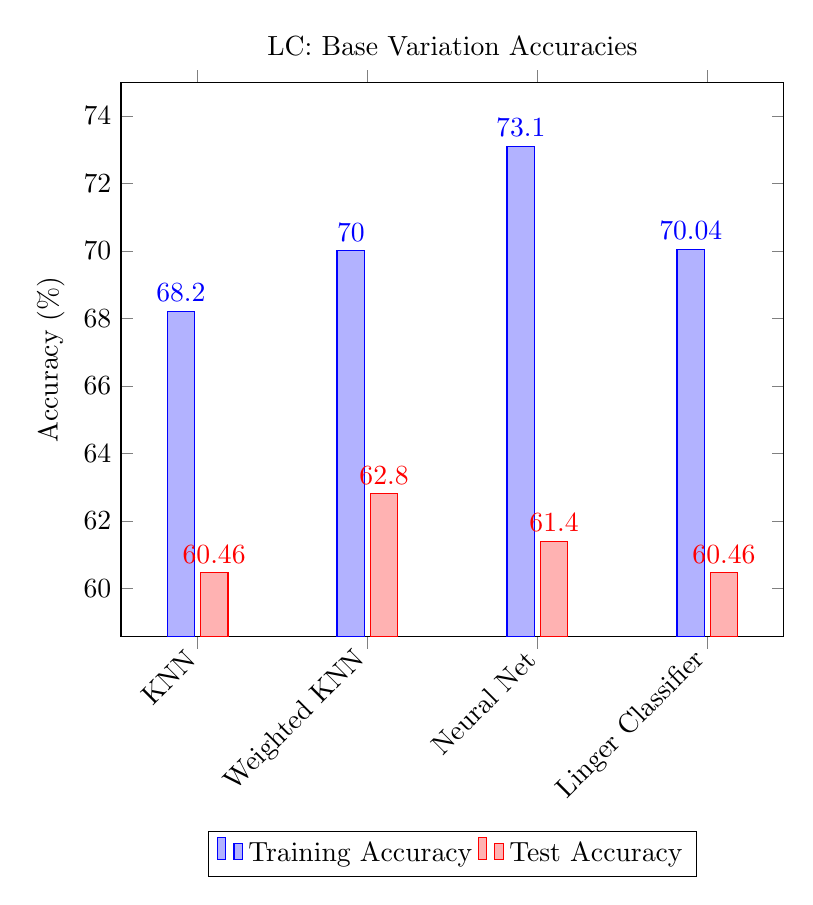
\begin{tikzpicture}
    \begin{axis}[
        ybar,
        enlargelimits=0.15,
        legend style={at={(0.5,-0.35)},
          anchor=north,legend columns=-1},
        ylabel={Accuracy (\%)},
        symbolic x coords={KNN,Weighted KNN,Neural Net,Linger Classifier},
        xtick=data,
        nodes near coords,
        nodes near coords align={vertical},
        x tick label style={rotate=45,anchor=east},
        title={LC: Base Variation Accuracies}
        ]
    \addplot coordinates {(KNN,68.2) (Weighted KNN,70.0) (Neural Net,73.1) (Linger Classifier,70.04)};
    \addplot coordinates {(KNN,60.46) (Weighted KNN,62.8) (Neural Net,61.4) (Linger Classifier,60.46)};
    \legend{Training Accuracy,Test Accuracy}
    \end{axis}
\end{tikzpicture}

\subsubsection{(LCV1) Results}

\begin{table}[H]
    \centering
    \caption{Best Parameters for Classifiers (LCV1)}
    \label{tab:best_parameters_combined_LCV1}
    \begin{tabular}{lll}
    \toprule
    \textbf{Classifier} & \textbf{Hyperparameter} & \textbf{Value} \\
    \midrule
    \multicolumn{3}{l}{\textit{Common Parameters for Neural Net and Linger Classifier with Context (Variation 1)}} \\
    \midrule
    Neural Net / Linger Classifier & activation & relu \\
    Neural Net / Linger Classifier & alpha & 0.1 \\
    Neural Net / Linger Classifier & beta\_1 & 0.9 \\
    Neural Net / Linger Classifier & beta\_2 & 0.999 \\
    Neural Net / Linger Classifier & early\_stopping & True \\
    Neural Net / Linger Classifier & hidden\_layer\_sizes & (300, 200, 100) \\
    Neural Net / Linger Classifier & learning\_rate\_init & 0.01 \\
    Neural Net / Linger Classifier & max\_iter & 1500 \\
    Neural Net / Linger Classifier & solver & adam \\
    Neural Net / Linger Classifier & validation\_fraction & 0.3 \\
    \midrule
    \multicolumn{3}{l}{\textit{KNN Classifier Specific}} \\
    \midrule
    KNN & n\_neighbors & 2 \\
    \midrule
    \multicolumn{3}{l}{\textit{Weighted KNN Classifier Specific}} \\
    \midrule
    Weighted KNN & n\_neighbors & 7 \\
    \midrule
    \multicolumn{3}{l}{\textit{Linger Classifier with Context (Variation 1) Specific}} \\
    \midrule
    Linger Classifier & addition\_of\_context & True \\
    Linger Classifier & additional\_results\_column & False \\
    Linger Classifier & duplicated\_on\_distance & False \\
    Linger Classifier & n\_neighbours\_1 & 17 \\
    Linger Classifier & n\_neighbours\_2 & 17 \\
    Linger Classifier & weighted\_knn & False \\
    \bottomrule
    \end{tabular}
\end{table}
\clearpage

\begin{table}[H]
    \centering
    \caption{Average Training and Test Accuracy Results for Classifiers (LCV1)}
    \label{tab:average_results_LCV1}
    \begin{tabular}{lll}
    \toprule
    \textbf{Classifier} & \textbf{Training Accuracy (\%)} & \textbf{Test Accuracy (\%)} \\
    \midrule
    KNN Classifier & $68.24$ & $60.47$ \\
    Weighted KNN Classifier & $70.00$ & $62.79$ \\
    Neural Network Classifier & $72.79$ & $64.53$ \\
    Linger Classifier & $69.41$ & $65.70$ \\
    \bottomrule
    \end{tabular}
\end{table}
\clearpage

\subsubsection{(LCV1) Analysis}
In LCV1, the inclusion of context, (setting $addition_of_context == \text{True}$) for the \texttt{LingerClassifier} led to a noticeable improvement in test accuracy for the Linger Classifier, 
outperforming the NN in test accuracy while maintaining competitive training accuracy. 
This improvement underscores the value of incorporating contextual information into the model, potentially enhancing its ability to generalize from training to test data.

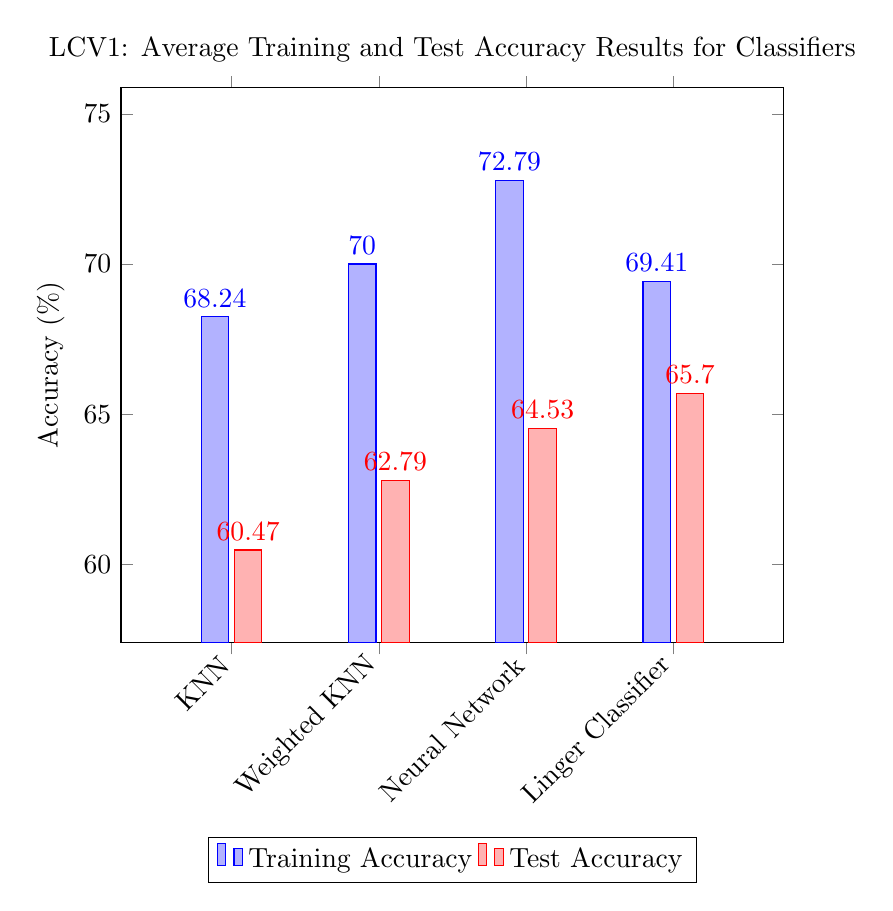
\begin{tikzpicture}
    \begin{axis}[
        ybar,
        enlargelimits=0.25,
        legend style={at={(0.5,-0.35)},
          anchor=north,legend columns=-1},
        ylabel={Accuracy (\%)},
        symbolic x coords={KNN, Weighted KNN, Neural Network, Linger Classifier},
        xtick=data,
        nodes near coords,
        nodes near coords align={vertical},
        x tick label style={rotate=45,anchor=east},
        title={LCV1: Average Training and Test Accuracy Results for Classifiers}
        ]
    \addplot coordinates {(KNN,68.24) (Weighted KNN,70.00) (Neural Network,72.79) (Linger Classifier,69.41)};
    \addplot coordinates {(KNN,60.47) (Weighted KNN,62.79) (Neural Network,64.53) (Linger Classifier,65.70)};
    \legend{Training Accuracy,Test Accuracy}
    \end{axis}
\end{tikzpicture}

\subsubsection{(LCV2) Results}

\begin{table}[H]
    \centering
    \caption{Best Parameters for Classifiers (LCV2)}
    \label{tab:best_parameters_combined_LCV2}
    \begin{tabular}{lll}
    \toprule
    \textbf{Classifier} & \textbf{Hyperparameter} & \textbf{Value} \\
    \midrule
    \multicolumn{3}{l}{\textit{Common Parameters for Neural Net and Linger Classifier, Duplication using Distance (Variation 2)}} \\
    \midrule
    Neural Net / Linger Classifier & activation & relu \\
    Neural Net / Linger Classifier & alpha & 0.1 \\
    Neural Net / Linger Classifier & beta\_1 & 0.9 \\
    Neural Net / Linger Classifier & beta\_2 & 0.995 \\
    Neural Net / Linger Classifier & early\_stopping & True \\
    Neural Net / Linger Classifier & hidden\_layer\_sizes & (300, 200, 100) \\
    Neural Net / Linger Classifier & learning\_rate\_init & 0.01 \\
    Neural Net / Linger Classifier & max\_iter & 1000 \\
    Neural Net / Linger Classifier & solver & adam \\
    Neural Net / Linger Classifier & validation\_fraction & 0.3 \\
    \midrule
    \multicolumn{3}{l}{\textit{KNN Classifier Specific}} \\
    \midrule
    KNN & n\_neighbors & 2 \\
    \midrule
    \multicolumn{3}{l}{\textit{Weighted KNN Classifier Specific}} \\
    \midrule
    Weighted KNN & n\_neighbors & 7 \\
    \midrule
    \multicolumn{3}{l}{\textit{Linger Classifier, Duplication using Distance (Variation 2) Specific}} \\
    \midrule
    Linger Classifier & addition\_of\_context & False \\
    Linger Classifier & additional\_distance\_column & False \\
    Linger Classifier & duplicated\_on\_distance & True \\
    Linger Classifier & n\_neighbours\_1 & 21 \\
    Linger Classifier & n\_neighbours\_2 & 13 \\
    Linger Classifier & weighted\_knn & False \\
    \bottomrule
    \end{tabular}
\end{table}
\clearpage

\begin{table}[H]
    \centering
    \caption{Average Training and Test Accuracy Results for Classifiers (LCV2)}
    \label{tab:average_results_LCV2}
    \begin{tabular}{lll}
    \toprule
    \textbf{Classifier} & \textbf{Training Accuracy (\%)} & \textbf{Test Accuracy (\%)} \\
    \midrule
    KNN Classifier & $68.24$ & $60.47$ \\
    Weighted KNN Classifier & $70.00$ & $62.79$ \\
    Neural Network Classifier & $71.29$ & $67.91$ \\
    Linger Classifier & $67.29$ & $69.30$ \\
    \bottomrule
    \end{tabular}
\end{table}
\clearpage

\subsubsection{(LCV2) Analysis}
Variation 2, focusing on duplicating data based on distance ($duplicated_on_distance == \text{True}$), yielded the most significant test accuracy increase for the \texttt{LingerClassifier}, 
surpassing even the Neural Network. This strategy might have provided a more nuanced understanding of the dataset's structure, aiding the model in better capturing the underlying patterns. 
This result suggests that data duplication based on distance could be a powerful method for improving model performance, especially in classification tasks where spatial relationships within the 
data are informative.

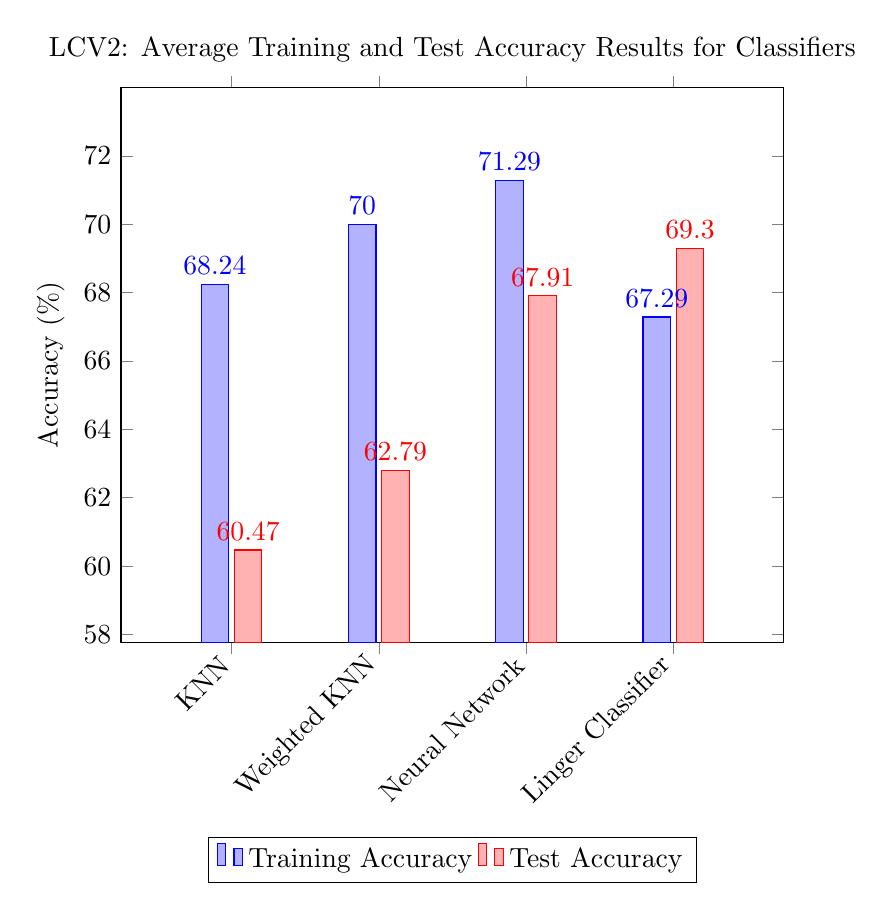
\begin{tikzpicture}
    \begin{axis}[
        ybar,
        enlargelimits=0.25,
        legend style={at={(0.5,-0.35)},
          anchor=north,legend columns=-1},
        ylabel={Accuracy (\%)},
        symbolic x coords={KNN, Weighted KNN, Neural Network, Linger Classifier},
        xtick=data,
        nodes near coords,
        nodes near coords align={vertical},
        x tick label style={rotate=45,anchor=east},
        title={LCV2: Average Training and Test Accuracy Results for Classifiers}
        ]
    \addplot coordinates {(KNN,68.24) (Weighted KNN,70.00) (Neural Network,71.29) (Linger Classifier,67.29)};
    \addplot coordinates {(KNN,60.47) (Weighted KNN,62.79) (Neural Network,67.91) (Linger Classifier,69.30)};
    \legend{Training Accuracy,Test Accuracy}
    \end{axis}
\end{tikzpicture}

\subsubsection{(LCV3) Results}

\begin{table}[H]
    \centering
    \caption{Best Parameters for Classifiers (LCV3)}
    \label{tab:best_parameters_combined_LCV3}
    \begin{tabular}{lll}
    \toprule
    \textbf{Classifier} & \textbf{Hyperparameter} & \textbf{Value} \\
    \midrule
    \multicolumn{3}{l}{\textit{Common Parameters for Neural Net and Linger Classifier, Additional Distance Column (Variation 3)}} \\
    \midrule
    Neural Net / Linger Classifier & activation & relu \\
    Neural Net / Linger Classifier & alpha & 0.001 \\
    Neural Net / Linger Classifier & beta\_1 & 0.99 \\
    Neural Net / Linger Classifier & beta\_2 & 0.999 \\
    Neural Net / Linger Classifier & early\_stopping & True \\
    Neural Net / Linger Classifier & hidden\_layer\_sizes & (300, 200, 100) \\
    Neural Net / Linger Classifier & learning\_rate\_init & 0.01 \\
    Neural Net / Linger Classifier & max\_iter & 1000 \\
    Neural Net / Linger Classifier & solver & adam \\
    Neural Net / Linger Classifier & validation\_fraction & 0.3 \\
    \midrule
    \multicolumn{3}{l}{\textit{KNN Classifier Specific}} \\
    \midrule
    KNN & n\_neighbors & 2 \\
    \midrule
    \multicolumn{3}{l}{\textit{Weighted KNN Classifier Specific}} \\
    \midrule
    Weighted KNN & n\_neighbors & 7 \\
    \midrule
    \multicolumn{3}{l}{\textit{Linger Classifier with Additional Distance Column (Variation 3) Specific}} \\
    \midrule
    Linger Classifier & addition\_of\_context & False \\
    Linger Classifier & additional\_distance\_column & True \\
    Linger Classifier & duplicated\_on\_distance & False \\
    Linger Classifier & n\_neighbours\_1 & 21 \\
    Linger Classifier & n\_neighbours\_2 & 13 \\
    Linger Classifier & weighted\_knn & False \\
    \bottomrule
    \end{tabular}
\end{table}
\clearpage

\begin{table}[H]
    \centering
    \caption{Average Training and Test Accuracy Results for Classifiers (LCV3)}
    \label{tab:average_results_LCV3}
    \begin{tabular}{lll}
    \toprule
    \textbf{Classifier} & \textbf{Training Accuracy (\%)} & \textbf{Test Accuracy (\%)} \\
    \midrule
    KNN Classifier & $68.24$ & $60.47$ \\
    Weighted KNN Classifier & $70.00$ & $62.79$ \\
    Neural Network Classifier & $71.06$ & $67.44$ \\
    Linger Classifier & $67.65$ & $60.93$ \\
    \bottomrule
    \end{tabular}
\end{table}
\clearpage
\subsubsection{(LCV3) Analysis}
The third variation, which introduced an additional distance column ($additional_distance_column == \text{True}$), did not lead to 
improvement in test accuracy for the \texttt{LingerClassifier} compared to LCV2 but maintained a competitive edge against the base NN model. 
This indicates that while adding distance-based features can be beneficial, there may be diminishing returns to complexity, or specific dataset characteristics 
may not fully leverage this type of information.

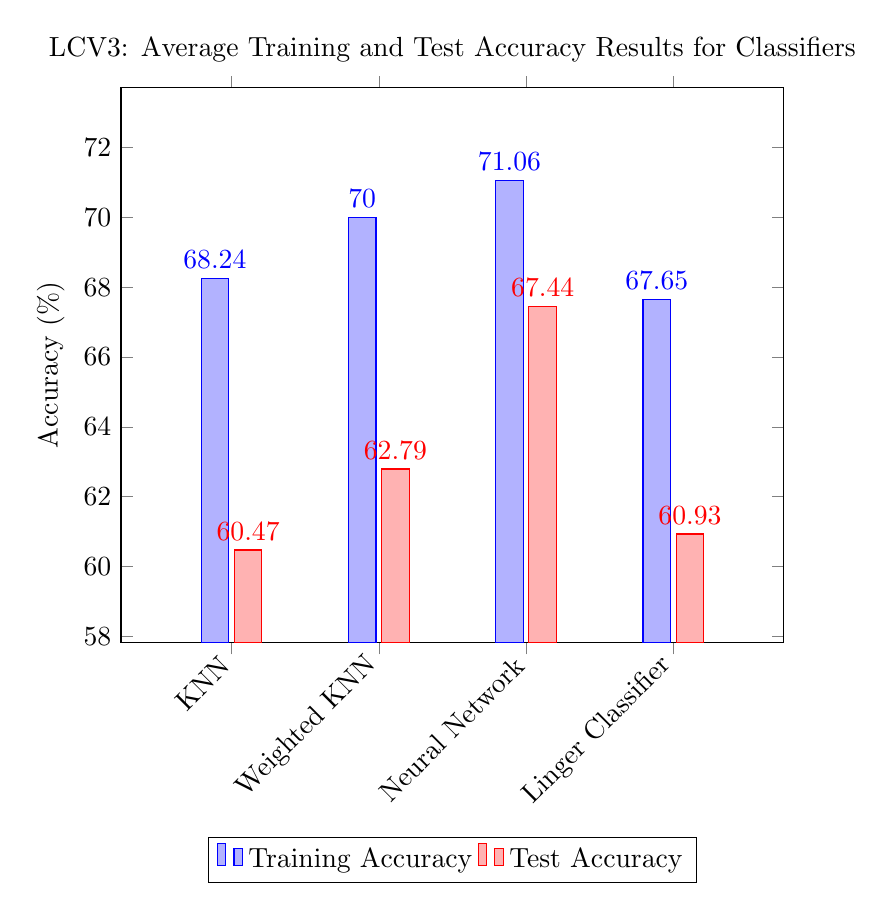
\begin{tikzpicture}
    \begin{axis}[
        ybar,
        enlargelimits=0.25,
        legend style={at={(0.5,-0.35)},
          anchor=north,legend columns=-1},
        ylabel={Accuracy (\%)},
        symbolic x coords={KNN, Weighted KNN, Neural Network, Linger Classifier},
        xtick=data,
        nodes near coords,
        nodes near coords align={vertical},
        x tick label style={rotate=45,anchor=east},
        title={LCV3: Average Training and Test Accuracy Results for Classifiers}
        ]
    \addplot coordinates {(KNN,68.24) (Weighted KNN,70.00) (Neural Network,71.06) (Linger Classifier,67.65)};
    \addplot coordinates {(KNN,60.47) (Weighted KNN,62.79) (Neural Network,67.44) (Linger Classifier,60.93)};
    \legend{Training Accuracy,Test Accuracy}
    \end{axis}
\end{tikzpicture}

\subsubsection{(LIC)}
\subsubsection{(LICV1)}
\subsubsection{(LICV2)}

\subsubsection{Concluding Remarks}

\subsection{Experiment 2: Abalone Dataset Regression}
\subsubsection{Methodology}

In Experiment 2, we explored regression tasks on the Abalone dataset with a two-step approach. 
Initially, a neural network (NN) regressor was trained using grid search and cross-validation to identify optimal hyperparameter combinations. 
These selected hyperparameters were then applied to train a \texttt{LingerRegressor} (LR) and its variants, targeting improved robustness, 
with their performance evaluated across four runs. Additionally, to benchmark the \texttt{LingerRegressor}'s performance, K-Nearest Neighbors (KNN), 
weighted KNN, and NN models were similarly assessed on the dataset. The results section will detail the hyperparameters and performance metrics obtained from Experiment 2.

\subsubsection{Tested Hyperparameters}

\begin{table}[H]
    \centering
    \caption{Tested Hyperparameters for Neural Network and Linger Regressor}
    \label{tab:hyperparameters_abalone}
    \begin{tabular}{|l|l|}
    \hline
    \textbf{Hyperparameter} & \textbf{Values} \\ \hline
    \multicolumn{2}{|c|}{\textbf{Neural Network}} \\ \hline
    Hidden Layer Sizes & (256, 128), (128, 64), (200, 100), (300, 200, 100) \\ \hline
    Activation & relu \\ \hline
    Alpha & 0.0001, 0.001, 0.01, 0.1 \\ \hline
    Max Iterations & 2000 \\ \hline
    Early Stopping & True \\ \hline
    Validation Fraction & 0.1 \\ \hline
    Learning Rate Init & 0.001, 0.01, 0.1 \\ \hline
    Solver & adam, sgd \\ \hline
    Beta 1 & 0.9, 0.95, 0.99 \\ \hline
    Beta 2 & 0.999, 0.995, 0.9 \\ \hline
    \multicolumn{2}{|c|}{\textbf{Linger Regressor}} \\ \hline
    N Neighbours 1 & 2, 5, 7, 10, 13, 15, 17, 21 \\ \hline
    N Neighbours 2 & 2, 5, 7, 10, 13, 15, 17, 21 \\ \hline
    Weighted KNN & False \\ \hline
    Additional Distance Column & True, False \\ \hline
    Duplicated on Distance & True, False \\ \hline
    Addition of Context & True, False \\ \hline
    \end{tabular}
\end{table}
\clearpage

\subsubsection{(LR) Results}

\begin{table}[H]
    \centering
    \caption{Best Parameters for Regressors (LR)}
    \label{tab:best_parameters_combined_LR}
    \begin{tabular}{lll}
    \toprule
    \textbf{Regressor} & \textbf{Hyperparameter} & \textbf{Value} \\
    \midrule
    \multicolumn{3}{l}{\textit{Common Parameters for Neural Net Regressor and Linger Regressor}} \\
    \midrule
    Neural Net / Linger Regressor & Activation & relu \\
    Neural Net / Linger Regressor & Alpha & 0.01 \\
    Neural Net / Linger Regressor & Beta 1 & 0.95 \\
    Neural Net / Linger Regressor & Beta 2 & 0.9 \\
    Neural Net / Linger Regressor & Early Stopping & True \\
    Neural Net / Linger Regressor & Hidden Layer Sizes & (200, 100) \\
    Neural Net / Linger Regressor & Learning Rate Init & 0.01 \\
    Neural Net / Linger Regressor & Max Iter & 2000 \\
    Neural Net / Linger Regressor & Solver & sgd \\
    Neural Net / Linger Regressor & Validation Fraction & 0.1 \\
    \midrule
    \multicolumn{3}{l}{\textit{KNN Regressor Specific}} \\
    \midrule
    KNN Regressor & n\_neighbors & 17 \\
    \midrule
    \multicolumn{3}{l}{\textit{Weighted KNN Regressor Specific}} \\
    \midrule
    Weighted KNN Regressor & n\_neighbors & 21 \\
    \midrule
    \multicolumn{3}{l}{\textit{Linger Regressor Specific}} \\
    \midrule
    Linger Regressor & Addition of Context & False \\
    Linger Regressor & Additional Distance Column & False \\
    Linger Regressor & Duplicated on Distance & False \\
    Linger Regressor & n\_Neighbours\_1 & 5 \\
    Linger Regressor & n\_Neighbours\_2 & 21 \\
    Linger Regressor & Weighted KNN & False \\
    \bottomrule
    \end{tabular}
\end{table}
\clearpage

\begin{table}[H]
    \centering
    \caption{Average Training and Test Negative Mean Squared Error Results (NMSE) for Regressors (LR)}
    \label{tab:average_results_LR}
    \begin{tabular}{lll}
    \toprule
    \textbf{Regressor} & \textbf{Average Training NMSE} & \textbf{Average Test NMSE} \\
    \midrule
    KNN Regressor & $-1.95857$ & $-1.92999$ \\
    Weighted KNN Regressor & $-1.9567$ & $-1.8717$ \\
    Neural Net Regressor & $-1.92956$ & $-1.89454$ \\
    Linger Regressor & $-1.89797$ & $-1.83486$ \\
    \bottomrule
    \end{tabular}
\end{table}
\clearpage
\subsubsection{(LR) Analysis}

In an examination of the \texttt{LingerRegressor}'s performance across five iterations, it became evident that this model, even in its unvaried form, consistently outshined its counterparts during both the training and testing phases. 
This superior performance underscores the efficacy of its unique "learning from differences" approach, adeptly uncovering and leveraging the dataset's underlying patterns. 
Notably, while extensive hyperparameter optimization was applied to the Neural Network models, the \texttt{LingerRegressor} has yet to
 undergo a similar level of fine-tuning due to resource limitiations. 
 This observation hints at the untapped potential of the \texttt{LingerRegressor}, suggesting that with targeted hyperparameter 
 adjustments and the exploration of variations, there could be a significant opportunity to further enhance its performance.

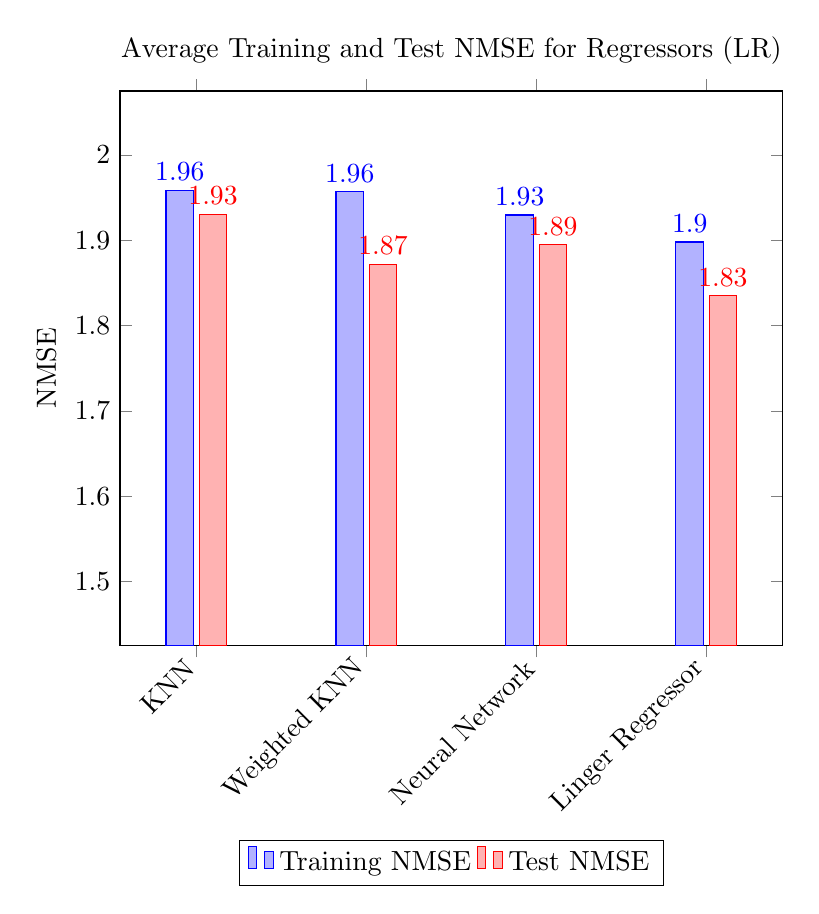
\begin{tikzpicture}
    \begin{axis}[
        ybar,
        enlargelimits=0.15,
        legend style={at={(0.5,-0.35)},
          anchor=north,legend columns=-1},
        ylabel={NMSE},
        ymin=1.5, ymax=2, % Setting the y-axis limits
        symbolic x coords={KNN, Weighted KNN, Neural Network, Linger Regressor},
        xtick=data,
        nodes near coords,
        nodes near coords align={vertical},
        x tick label style={rotate=45,anchor=east},
        title={Average Training and Test NMSE for Regressors (LR)}
        ]
    \addplot coordinates {(KNN,1.95857) (Weighted KNN,1.9567) (Neural Network,1.92956) (Linger Regressor,1.89797)};
    \addplot coordinates {(KNN,1.92999) (Weighted KNN,1.8717) (Neural Network,1.89454) (Linger Regressor,1.83486)};
    \legend{Training NMSE,Test NMSE}
    \end{axis}
\end{tikzpicture}
\subsubsection{(LRV1) Results}

\begin{table}[H]
    \centering
    \caption{Best Parameters for Regressors (LRV1)}
    \label{tab:best_parameters_combined_LRV1}
    \begin{tabular}{lll}
    \toprule
    \textbf{Regressor} & \textbf{Hyperparameter} & \textbf{Value} \\
    \midrule
    \multicolumn{3}{l}{\textit{Common Parameters for Neural Net Regressor and Linger Regressor}} \\
    \midrule
    Neural Net / Linger Regressor & Activation & relu \\
    Neural Net / Linger Regressor & Alpha & 0.1 \\
    Neural Net / Linger Regressor & Beta 1 & 0.99 \\
    Neural Net / Linger Regressor & Beta 2 & 0.9 \\
    Neural Net / Linger Regressor & Early Stopping & True \\
    Neural Net / Linger Regressor & Hidden Layer Sizes & (300, 200, 100) \\
    Neural Net / Linger Regressor & Learning Rate Init & 0.01 \\
    Neural Net / Linger Regressor & Max Iter & 2000 \\
    Neural Net / Linger Regressor & Solver & sgd \\
    Neural Net / Linger Regressor & Validation Fraction & 0.1 \\
    \midrule
    \multicolumn{3}{l}{\textit{KNN Regressor Specific}} \\
    \midrule
    KNN Regressor & n\_neighbors & 17 \\
    \midrule
    \multicolumn{3}{l}{\textit{Weighted KNN Regressor Specific}} \\
    \midrule
    Weighted KNN Regressor & n\_neighbors & 21 \\
    \midrule
    \multicolumn{3}{l}{\textit{Linger Regressor Specific}} \\
    \midrule
    Linger Regressor & Addition of Context & True \\
    Linger Regressor & Additional Distance Column & False \\
    Linger Regressor & Duplicated on Distance & False \\
    Linger Regressor & n\_neighbours\_1 & 2 \\
    Linger Regressor & n\_neighbours\_2 & 21 \\
    Linger Regressor & Weighted KNN & False \\
    \bottomrule
    \end{tabular}
\end{table}
\clearpage

\begin{table}[H]
    \centering
    \caption{Average Training and Test Negative Mean Squared Error Results for Regressors (LRV1)}
    \label{tab:average_results_LRV1}
    \begin{tabular}{lll}
    \toprule
    \textbf{Regressor} & \textbf{Average Training NMSE} & \textbf{Average Test NMSE} \\
    \midrule
    KNN Regressor & $-1.9586$ & $-1.9300$ \\
    Weighted KNN Regressor & $-1.9567$ & $-1.8717$ \\
    Neural Net Regressor & $-1.8848$ & $-1.8234$ \\
    Linger Regressor & $-1.9420$ & $-1.8697$ \\
    \bottomrule
    \end{tabular}
\end{table}
\clearpage
\subsubsection{(LRV1) Analysis}
The exploration of the \texttt{LingerRegressor} in its variation one (LRV1) configuration, incorporating the addition of context as a new parameter,
has yielded intriguing insights. This variation maintained the \texttt{LingerRegressor}'s competitive edge, particularly in the testing phase, 
where it achieved a lower Negative Mean Squared Error (NMSE) compared to its baseline and even outperformed the Neural Net Regressors training results. 
The selected hyperparameters for LRV1—emphasizing a higher alpha and a shift in beta values—suggest an optimized balance between model complexity and regularization, 
contributing to its enhanced performance. Remarkably, the Linger Regressor’s capacity to integrate context into its predictive process appears not especially benefit its ability to generalize, 
as evidenced by its test (NMSE) scores, as they are very similar and slightly worse than the base version.

This phase of experimentation underscores the substantial impact that tailored hyperparameter adjustments and strategic feature incorporation can have on model performance. 
Despite the Neural Net Regressor undergoing extensive hyperparameter optimization, the Linger Regressor, with its focused enhancements in LRV1, demonstrates that thoughtful model refinement alter performance gains.
The results from LRV1 not only reaffirm the \texttt{LingerRegressor}'s potential in leveraging complex patterns within the data but also spotlight the promising avenue that lies in further exploring and fine-tuning this model’s capabilities.

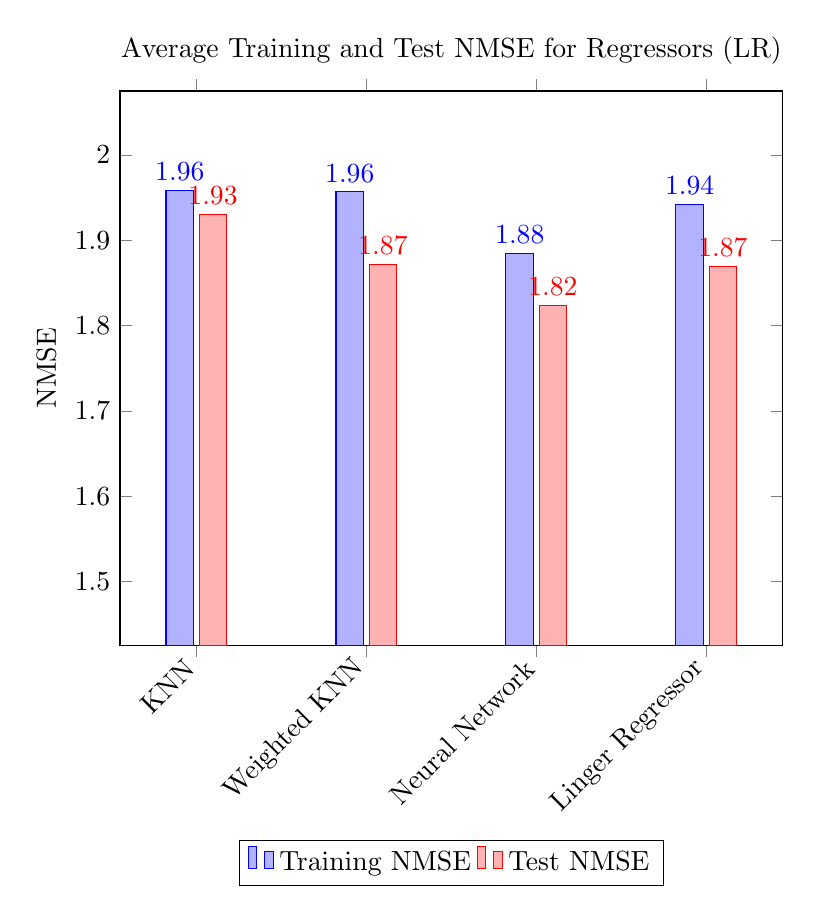
\begin{tikzpicture}
    \begin{axis}[
        ybar,
        enlargelimits=0.15,
        legend style={at={(0.5,-0.35)},
          anchor=north,legend columns=-1},
        ylabel={NMSE},
        ymin=1.5, ymax=2, % Setting the y-axis limits
        symbolic x coords={KNN, Weighted KNN, Neural Network, Linger Regressor},
        xtick=data,
        nodes near coords,
        nodes near coords align={vertical},
        x tick label style={rotate=45,anchor=east},
        title={Average Training and Test NMSE for Regressors (LR)}
        ]
    \addplot coordinates {(KNN,1.9586) (Weighted KNN,1.9567) (Neural Network,1.8848) (Linger Regressor,1.9420)};
    \addplot coordinates {(KNN,1.9300) (Weighted KNN,1.8717) (Neural Network,1.8234) (Linger Regressor,1.8697)};
    \legend{Training NMSE,Test NMSE}
    \end{axis}
\end{tikzpicture}
\subsubsection{(LRV2) Results}

\subsubsection{(LRV3)}
\subsubsection{(LIR)}

\begin{table}[H]
    \centering
    \caption{Updated Best Parameters for Regressors (LRV1)}
    \label{tab:updated_best_parameters_combined_LRV1}
    \begin{tabular}{lll}
    \toprule
    \textbf{Regressor} & \textbf{Hyperparameter} & \textbf{Value} \\
    \midrule
    \multicolumn{3}{l}{\textit{Common Parameters for Neural Net Regressor and Linger Implicit Regressor}} \\
    \midrule
    Basic Neural Network / Linger Regressor & Activation & relu \\
    Basic Neural Network / Linger Regressor & Alpha & 0.01 \\
    Basic Neural Network / Linger Regressor & Beta 1 & 0.9 \\
    Basic Neural Network / Linger Regressor & Beta 2 & 0.9 \\
    Basic Neural Network / Linger Regressor & Early Stopping & True \\
    Basic Neural Network / Linger Regressor & Hidden Layer Sizes & (128, 64) \\
    Basic Neural Network / Linger Regressor & Learning Rate Init & 0.01 \\
    Basic Neural Network / Linger Regressor & Max Iter & 2000 \\
    Basic Neural Network / Linger Regressor & Solver & sgd \\
    Basic Neural Network / Linger Regressor & Validation Fraction & 0.1 \\
    \midrule
    \multicolumn{3}{l}{\textit{KNN Regressor Specific}} \\
    \midrule
    KNN Regressor & n\_neighbors & 21 \\
    \midrule
    \multicolumn{3}{l}{\textit{Weighted KNN Regressor Specific}} \\
    \midrule
    Weighted KNN Regressor & n\_neighbors & 21 \\
    \midrule
    \multicolumn{3}{l}{\textit{Linger Regressor Specific}} \\
    \midrule
    Linger Regressor & n\_segments & 3 \\
    Linger Regressor & equal\_division & True \\
    Linger Regressor & n\_neighbors\_1 & 21 \\
    Linger Regressor & n\_neighbors\_2 & 13 \\
    Linger Regressor & Random Pairs & False \\
    Linger Regressor & Single Pair & False \\
    \bottomrule
    \end{tabular}
\end{table}
\subsubsection{(LIRV1)}
\subsubsection{(LIRV2)}

\subsection{Experiment 3: Raisin Dataset Classification}
\subsubsection{Methodology}
In Experiment 3, we conducted classification tasks on the Raisin dataset from \cite{uciDatasets}, specifically the dataset \cite{misc_raisin_850} using a two-step methodology. Initially, we trained a neural network (NN) classifier 
through grid search and cross-validation to determine the optimal hyperparameters. These hyperparameters were then applied to train a \texttt{LingerClassifier} (LC) 
and its variants for improved robustness, tested across five runs.
For comparative analysis, we also evaluated the performance of K-Nearest Neighbors (KNN), 
weighted (KNN), and (NN) on the same dataset. The sections below detail the hyperparameters selected and the test accuracies achieved.

\subsubsection{Tested Hyperparameters}

\begin{table}[H]
    \centering
    \caption{Tested Hyperparameters for Neural Network and Linger Regressor}
    \label{tab:hyperparameters_raisin}
    \begin{tabular}{|l|l|}
    \hline
    \textbf{Hyperparameter} & \textbf{Values} \\ \hline
    \multicolumn{2}{|c|}{\textbf{Neural Network}} \\ \hline
    Hidden Layer Sizes & (256, 128), (128, 64), (200, 100), (300, 200, 100), (400, 300, 200, 100) \\ \hline
    Activation & identity, logistic, tanh, relu \\ \hline
    Alpha & 0.0001, 0.001, 0.01, 0.1 \\ \hline
    Max Iterations & 1500, 2000 \\ \hline
    Early Stopping & True \\ \hline
    Validation Fraction & 0.1, 0.2, 0.3 \\ \hline
    Learning Rate Init & 0.001, 0.01, 0.1 \\ \hline
    Solver & adam, sgd \\ \hline
    Beta 1 & 0.9, 0.95, 0.99 \\ \hline
    Beta 2 & 0.999, 0.995, 0.9 \\ \hline
    \multicolumn{2}{|c|}{\textbf{Linger Regressor}} \\ \hline
    N Neighbours 1 & 2, 5, 7, 10, 13, 15, 17, 21 \\ \hline
    N Neighbours 2 & 2, 5, 7, 10, 13, 15, 17, 21 \\ \hline
    Weighted KNN & False \\ \hline
    Additional Distance Column & True, False \\ \hline
    Duplicated on Distance & True, False \\ \hline
    Addition of Context & True, False \\ \hline
    \end{tabular}
\end{table}
\clearpage

\subsubsection{(LC) Results}

\begin{table}[H]
    \centering
    \caption{Best Parameters for Classifiers (LC)}
    \label{tab:best_parameters_combined_LC_Raisin}
    \begin{tabular}{lll}
    \toprule
    \textbf{Classifier} & \textbf{Hyperparameter} & \textbf{Value} \\
    \midrule
    \multicolumn{3}{l}{\textit{Common Parameters for Neural Net Classifier and Linger Classifier}} \\
    \midrule
    Neural Net / Linger Classifier & Activation & identity \\
    Neural Net / Linger Classifier & Alpha & 0.1 \\
    Neural Net / Linger Classifier & Beta 1 & 0.95 \\
    Neural Net / Linger Classifier & Beta 2 & 0.999 \\
    Neural Net / Linger Classifier & Early Stopping & True \\
    Neural Net / Linger Classifier & Hidden Layer Sizes & (200, 100) \\
    Neural Net / Linger Classifier & Learning Rate Init & 0.01 \\
    Neural Net / Linger Classifier & Max Iter & 2000 \\
    Neural Net / Linger Classifier & Solver & adam \\
    Neural Net / Linger Classifier & Validation Fraction & 0.2 \\
    \midrule
    \multicolumn{3}{l}{\textit{KNN Classifier Specific}} \\
    \midrule
    KNN Classifier & n\_neighbors & 13 \\
    \midrule
    \multicolumn{3}{l}{\textit{Weighted KNN Classifier Specific}} \\
    \midrule
    Weighted KNN Classifier & n\_neighbors & 13 \\
    \midrule
    \multicolumn{3}{l}{\textit{Linger Classifier Specific}} \\
    \midrule
    Linger Classifier & Addition of Context & False \\
    Linger Classifier & Additional Distance Column & False \\
    Linger Classifier & Duplicated on Distance & False \\
    Linger Classifier & n\_neighbors\_1 & 5 \\
    Linger Classifier & n\_neighbors\_2 & 13 \\
    Linger Classifier & Weighted KNN & False \\
    \bottomrule
    \end{tabular}
\end{table}
\clearpage

\begin{table}[H]
    \centering
    \caption{Average Training and Test Accuracy Results for Classifiers (LC)}
    \label{tab:average_results_LC_Raisin}
    \begin{tabular}{lll}
    \toprule
    \textbf{Classifier} & \textbf{Average Training Accuracy (\%)} & \textbf{Average Test Accuracy (\%)} \\
    \midrule
    KNN Classifier & $91.718$ & $91$ \\
    Weighted KNN Classifier & $91.218$ & $91$ \\
    Neural Net Classifier & $94.098$ & $91$ \\
    Linger Classifier & $91.655$ & $90.5$ \\
    \bottomrule
    \end{tabular}
\end{table}

\subsubsection{(LC) Analysis}
\subsubsection{(LCV1) Results}
This was only run twice as there were constraints on resources during testing that resulted in less robust trials.

\begin{table}[H]
    \centering
    \caption{Best Parameters for Classifiers (LCV1)}
    \label{tab:best_parameters_combined_LCV1_Raisin}
    \begin{tabular}{lll}
    \toprule
    \textbf{Classifier} & \textbf{Hyperparameter} & \textbf{Value} \\
    \midrule
    \multicolumn{3}{l}{\textit{Common Parameters for Neural Net Classifier and Linger Classifier}} \\
    \midrule
    Neural Net / Linger Classifier & Activation & identity \\
    Neural Net / Linger Classifier & Alpha & 0.1 \\
    Neural Net / Linger Classifier & Beta 1 & 0.95 \\
    Neural Net / Linger Classifier & Beta 2 & 0.999 (0.9 for Linger Classifier) \\
    Neural Net / Linger Classifier & Early Stopping & True \\
    Neural Net / Linger Classifier & Hidden Layer Sizes & (200, 100) \\
    Neural Net / Linger Classifier & Learning Rate Init & 0.01 \\
    Neural Net / Linger Classifier & Max Iter & 2000 \\
    Neural Net / Linger Classifier & Solver & adam \\
    Neural Net / Linger Classifier & Validation Fraction & 0.2 (0.3 for Linger Classifier) \\
    \midrule
    \multicolumn{3}{l}{\textit{KNN Classifier Specific}} \\
    \midrule
    KNN Classifier & n\_neighbors & 13 \\
    \midrule
    \multicolumn{3}{l}{\textit{Weighted KNN Classifier Specific}} \\
    \midrule
    Weighted KNN Classifier & n\_neighbors & 13 \\
    \midrule
    \multicolumn{3}{l}{\textit{Linger Classifier Specific}} \\
    \midrule
    Linger Classifier & Addition of Context & True \\
    Linger Classifier & Additional Distance Column & False \\
    Linger Classifier & Duplicated on Distance & False \\
    Linger Classifier & n\_neighbors\_1 & 15 \\
    Linger Classifier & n\_neighbors\_2 & 21 \\
    Linger Classifier & Weighted KNN & False \\
    \bottomrule
    \end{tabular}
\end{table}
\clearpage

\begin{table}[H]
    \centering
    \caption{Average Training and Test Accuracy Results for Classifiers (LCV1)}
    \label{tab:average_results_LCV1_Raisin}
    \begin{tabular}{lll}
    \toprule
    \textbf{Classifier} & \textbf{Average Training Accuracy (\%)} & \textbf{Average Test Accuracy (\%)} \\
    \midrule
    KNN Classifier & $91.718$ & $91$ \\
    Weighted KNN Classifier & $91.218$ & $91$ \\
    Neural Net Classifier & $94.139$ & $90$ \\
    Linger Classifier & $91.843$ & $90.168$ \\
    \bottomrule
    \end{tabular}
\end{table}
\clearpage

\subsubsection{(LCV2)}
\subsubsection{(LCV3)}
\subsubsection{(LIC)}
\subsubsection{(LICV1)}
\subsubsection{(LICV2)}

\section{Discussion}

\chapter{Conclusions and Future Work}
\label{ch:Conclusions and Future Work}
This chapter outlines the additions made in our study, acknowledges its limitations, and proposes directions for future research to extend 
the work's applicability and efficiency across multiple domains

\section{Addressing Identified Limitations}
Our study, while insightful, recognizes certain limitations in its current scope and methodology. 
Future efforts should aim to surpass these through advanced algorithmic enhancements and the integration of novel data processing techniques, this could be implemented through 
Scikit-learn \cite{scikit}. Such improvements are anticipated to refine the learning process further, enhancing the models' overall performance and applicability.

\section{Broader Applicability}
Exploring the applicability of our approach to broader machine learning challenges represents a promising direction for future research. 
Adapting our models to handle unstructured data or complex, high-dimensional datasets could significantly broaden their utility, making them suitable for a wider range of applications.

\section{Integration with Emerging Technologies}
The potential integration of our models with emerging technologies, such as deep learning and reinforcement learning, offers exciting possibilities. 
Such integration could not only provide new insights and enhance model capabilities but also facilitate the use of these models in real-time applications or 
embedded systems where interpretability and efficiency are paramount.

\section{Scalability and Efficiency}
Investigating the scalability and efficiency of our models, especially in contexts involving large-scale datasets or distributed computing environments, is crucial. 
Future research could focus on optimizations that reduce training times or adaptations that leverage parallel processing architectures to improve performance.

\section{Cross-Domain Applications}
Examining the effectiveness of our models across different domains or for various types of prediction tasks could uncover new applications and opportunities for impact. 
This exploration might involve interdisciplinary research collaborations to adapt and evaluate our models in diverse contexts. 
Evaluating the learning from difference models with real time data.

\section{Exploring Other Categorical Similarity Measures}
Investigating alternative measures for assessing the similarity of categorical features could refine the process of generating and applying adaptation rules, 
potentially enhancing the accuracy and applicability of the Ensemble of Adaptations for Classification (EAC). As seen in the paper \cite{jalali2017learning}.

\bibliographystyle{plain}
\bibliography{references}

\end{document}
